% Do not change document class, margins, fonts, etc.
\documentclass[a4paper,oneside,bibliography=totoc]{scrbook}

% some useful packages (add more as needed)
\usepackage{scrhack}
\usepackage[utf8]{inputenc}
\usepackage{graphicx}
\usepackage{latexsym}
\usepackage{amsmath}
\usepackage{amssymb}
\usepackage{tabularx}
\usepackage{csquotes}
\usepackage{booktabs}
\usepackage{listings}
\usepackage{algorithm}
\counterwithin{algorithm}{chapter}
\usepackage{algorithmic}
\usepackage{csquotes}
\renewcommand{\algorithmiccomment}[1]{\hfill\textit{// #1}}
\usepackage[usenames,dvipsnames]{xcolor}
\usepackage[colorlinks,citecolor=Green]{hyperref}
\usepackage{lipsum}
\usepackage[printonlyused]{acronym}

% chicago citation style
\usepackage{natbib}
\bibliographystyle{chicagoa}
\setcitestyle{authoryear,round,semicolon,aysep={},yysep={,}} \let\cite\citep

% example enviroments (add more as needed)
\newtheorem{definition}{Definition} \newtheorem{proposition}{Proposition}

% Definition einer Turtle-Sprache
\lstdefinelanguage{Turtle}{
  morekeywords={@prefix,@base,a},
  morekeywords=[2]{ex,exp,rdfs},
  morestring=[b]",
  morestring=[b]',
  sensitive=true,
  basicstyle=\small\ttfamily,
  keywordstyle=\color{blue},
  keywordstyle=[2]\color{magenta},
  commentstyle=\color{gray}\itshape,
  stringstyle=\color{OliveGreen},
  columns=fullflexible,
  breaklines=true,
  breakatwhitespace=false,
  literate={:}{{{\color{orange}:}}}1,
}

% Definition einer SPARQL-Sprache
\lstdefinelanguage{SPARQL}{
  morekeywords={@prefix,@base,a,SELECT,WHERE},
  morekeywords=[2]{ex,exp,rdfs},
  morestring=[b]",
  morestring=[b]',
  sensitive=true,
  basicstyle=\small\ttfamily,
  keywordstyle=\color{blue},
  keywordstyle=[2]\color{magenta},
  commentstyle=\color{gray}\itshape,
  stringstyle=\color{OliveGreen},
  columns=fullflexible,
  breaklines=true,
  breakatwhitespace=false,
  literate={:}{{{\color{orange}:}}}1,
}

% Globales Styling für alle Listings
\lstset{
  language=Turtle,
  frame=single,
  numbers=left,
  numberstyle=\tiny\color{gray},
  numbersep=5pt,
  tabsize=2,
  captionpos=b,
  basicstyle=\small\ttfamily,
}

\begin{document}

\frontmatter
\subject{Master Thesis}
\title{CIExMAS: Closed Information Extraction using a Multi-Agent-System}
\author{Max Lautenbach\\
  (matriculation number 1980683)}
\date{18.08.2025}
\publishers{{\small Submitted to}\\
  Data and Web Science Group\\
  Dr.\ Sven Hertling\\
  University of Mannheim\\}
\maketitle

\chapter{Abstract}
Closed information extraction has so far relied mainly on fine tuned transformer models that require large training datasets. Large language models have been used for open information extraction, but their application to closed information extraction has not yet been explored, nor has the use of artificial intelligence agents in this domain. In this work, we introduce CIExMAS, a collection of modular architectures based on multi agent systems for closed information extraction without the need for fine tuning, designed as an exploratory framework to test a broad range of architectural setups and evaluate the general feasibility of multi agent systems in this domain. The best architecture comprises specialized agents for triple extraction, uniform resource identifier mapping and validation, supported by tools for integration with knowledge graphs. In the evaluation, CIExMAS achieved up to 80\% of the performance of current state of the art models, despite requiring no fine tuning. This result highlights the effectiveness of approaches based on artificial intelligence agents in closed information extraction and points to their potential as flexible, scalable and lightweight alternatives. As an initial study in this direction, CIExMAS lays the foundation for further research combining artificial intelligence agents and closed information extraction.

\begingroup%
\hypersetup{hidelinks}%
\tableofcontents%
\endgroup

\begingroup%
\hypersetup{hidelinks}%
\listoffigures%
\addcontentsline{toc}{chapter}{List of Figures}
\endgroup

\begingroup%
\hypersetup{hidelinks}%
\listoftables%
\addcontentsline{toc}{chapter}{List of Tables}
\endgroup

\chapter{List of Abbreviations}
\begin{acronym}
  \acro{AI}{artificial intelligence}
  \acro{BPE}{byte pair encoding}
  \acro{cIE}{closed information extraction}
  \acro{CoT}{chain of thought}
  \acro{CRM}{customer relationship management}
  \acro{DBMS}{database management system}
  \acro{GPT}{Generative Pre-trained Transformer}
  \acro{ICL}{in-context learning}
  \acro{IE}{information extraction}
  \acro{KG}{knowledge graph}
  \acro{LLM}{large language model}
  \acro{LLaMA}{Large Language Model Meta AI}
  \acro{LM}{language model}
  \acro{MAS}{multi-agent system}
  \acro{ML}{machine learning}
  \acro{MTEB}{Massive Text Embedding Benchmark}
  \acro{NLP}{natural language processing}
  \acro{OWL}{Web Ontology Language}
  \acro{PropEx}{property extraction}
  \acro{RAG}{retrieval augmented generation}
  \acro{RDF}{Resource Description Framework}
  \acro{RDFS}{Resource Description Framework Schema}
  \acro{ReAct}{Reasoning and Acting}
  \acro{SPARQL}{SPARQL Protocol and RDF Query Language}
  \acro{SSA}{Splitted Supervisor Architecture}
  \acro{SSSA}{Simplified Splitted Supervisor Architecture}
  \acro{URI}{Uniform Resource Identifier}
  \acro{VDBMS}{vector database management system}
\end{acronym}

\mainmatter

\chapter{Introduction}
\label{ch:introduction}

\Acp{LM} and especially modern \acp{LLM} have significantly improved the ability of machines to understand and generate human language. These models have enabled progress in various downstream tasks ranging from question answering to summarization and reasoning \cite{Brown2020}. However, their static training data limits their ability to incorporate new or domain-specific knowledge, a limitation known as the knowledge cutoff problem. Most \acp{LLM} are trained once on large corpora and as a result they have no built-in access to information that emerged after the end of their training period and cannot retrieve up-to-date or external knowledge out of the box \cite{Brown2020,Grattafiori2024}.

As a result there is a growing interest in structured external knowledge sources, especially \acp{KG}, to provide reliable and semantically rich context for generative models \cite{Korolov2025}. Knowledge graphs are a concept used to store knowledge in a form that allows machines to retrieve and interpret semantic relationships \cite{GomezPerez2017}. They are typically modeled as directed graphs where nodes represent real-world entities and edges define the relationships between these entities \cite{Paulheim2016}. Ontologies specify the types of entities and relationships and additionally provide logical constraints that govern how instances can be interpreted within a domain \cite{GomezPerez2017,Paulheim2016}. The increasing use of \ac{LLM}-based applications has therefore renewed attention on \acp{KG} as critical infrastructure for trustworthy and explainable \ac{AI} \cite{Korolov2025}.

At the same time this demand creates a practical challenge: many enterprise or domain-specific datasets have not yet been transformed into a knowledge graph. Most relevant knowledge is still locked in unstructured text documents, reports or communication logs \cite{Korolov2025}. To make this information accessible to downstream applications it must be transformed into structured representations that align with a predefined ontology or knowledge schema.

This transformation process leads directly to the research field of \ac{cIE}. As a specialized task within the broader area of \ac{IE}, \ac{cIE} focuses on extracting subject–predicate–object triples from text such that all components can be linked to valid entries in a target knowledge graph \cite{Josifoski2021}. This makes \ac{cIE} a crucial enabling technology for knowledge base population \cite{Josifoski2021}.

\section{Motivation and Problem Statement}
\label{sec:motivation}

The automatic extraction of structured information from text is a long-standing goal in natural language processing. This task, generally referred to as \ac{IE}, includes subtasks such as named entity recognition, entity linking, and relation extraction. These components aim to identify real-world entities in text, assign them canonical identifiers, and detect semantic relationships between them \cite{Zhao2024}.

\Ac{cIE} is a constrained subtask of \ac{IE}, where the goal is to extract subject–predicate–object triples that exactly match predefined entries in a \ac{KG}. In contrast to open \ac{IE} approaches, where relations may be freely expressed in natural language, \ac{cIE} requires strict alignment with the vocabulary and structure of a target ontology. This constraint makes \ac{cIE} especially relevant for applications that involve structured knowledge integration or automated \ac{KG} construction \cite{Josifoski2021}.

This tight coupling reduces reusability and makes it difficult to adapt systems to new domains or ontologies without significant retraining. Consequently, researchers are exploring more modular alternatives that promise better generalisation without the need for task-specific fine-tuning \cite{Shi2024}.

State-of-the-art models such as GenIE and synthIE model have shown that \ac{cIE} can be performed with very high accuracy, particularly when the models are fine-tuned on a high-quality dataset. However, \cite{Josifoski2021,Josifoski2023} demonstrate a limitation that models trained on one dataset do not generalize well to others (e.g., synthIE) even when the task and \ac{KG} structure remain similar. This lack of generalization highlights a key drawback of current \ac{IE} systems, which often rely on supervised fine-tuning and are closely coupled to a specific domain or knowledge graph.

To address such challenges, large language models have been explored for information extraction tasks in general, leveraging their strong \ac{ICL} capabilities. These capabilities allow \acp{LLM} to adapt to new tasks and domains based on a few examples or instructions provided at inference time, rather than requiring retraining. This property makes them a promising candidate for overcoming both the limited generalization and the need for extensive fine-tuning in current \ac{cIE} models.

While LLM-based approaches have shown promise for \ac{IE}, their potential for the more constrained setting of \ac{cIE} has not yet been systematically investigated. This opens up the possibility of solving \ac{cIE} through prompting alone, without any task-specific fine-tuning.

At the same time, recent work in agentic AI explores how \acp{LLM} can be used as decision engines in \acp{MAS} that interact via tool use, planning, and role-based coordination~\cite{OpenAI2025,Anthropic2024,Wiesinger2025}. These systems have shown promise for complex reasoning tasks and dynamic workflows. \citet{Shi2024} further demonstrate that even single-agent architectures can achieve state-of-the-art performance on \ac{IE} tasks.

These developments motivate the hypothesis that \acp{MAS} with \acp{LLM} as decision engines may offer an effective and generalizable approach to \ac{cIE}. Unlike monolithic pipelines or fine-tuned models, multi-agent architectures can decompose the task into modular roles such as entity extraction, \ac{URI} disambiguation, and triple validation while combining the flexibility of prompting with the ability to access external tools. This is especially relevant when generating \ac{KG}-ready triples, as these often require lookups or validation against the underlying graph structure. Such tool use is increasingly common in modern agentic frameworks \cite{OpenAI2025} and forms the foundation of the CIExMAS architecture proposed in this thesis.

\section{Research Questions and Objectives}
\label{sec:research_questions}

This thesis investigates whether \ac{cIE} can be solved effectively by \ac{LLM}-based \acp{MAS} without relying on model fine-tuning. The central idea is to test such systems as an alternative to traditional supervised fine-tuned \ac{cIE} models. These agents operate in distributed, role-based settings and coordinate through a shared plan or workflow, performing tasks such as entity and relation extraction, \ac{URI} matching, or validation by means of prompting and tool use.

The following research questions guide this investigation:

\begin{itemize}
  \item[\textbf{RQ1}] To what extent can \ac{LLM}-based \acp{MAS} perform closed information extraction on unstructured text?
  \item[\textbf{RQ2}] Which agentic architectures (e.g., single-agent, supervisor-agent, or agent networks) perform best for this task in terms of accuracy and robustness?
\end{itemize}

\section{Methodological Approach}
\label{sec:methodology}

To address these questions, this thesis presents CIExMAS, a closed information extraction multi-agent system. CIExMAS was developed through an iterative process that emphasised modularity and extensibility, but followed no rigid pipeline. Rather, agents and prompts were initially tested on a small sample set and improved step by step, using qualitative trace inspection and targeted adjustments. This empirical, trial-and-error driven strategy was followed by evaluation on a larger benchmark subset.

The system was implemented using the LangGraph framework, which provides abstractions for \ac{LLM}-based agent flows and tool orchestration, and served as the foundation for developing and testing several configurations. These configurations ranged from a single-agent to supervisor–worker hierarchies and decentralized agent networks. In all setups, the goal was to extract valid triples from unstructured documents using only prompt engineering and tool usage, without any model fine-tuning.

To evaluate this agentic approach, pre-trained snapshots of existing comparison models GenIE and the synthIE model were used. Both were run on the same subset of the synthIE dataset as the CIExMAS configurations, enabling a fair comparison. Performance was assessed using macro-F1 as well as entity-level precision, recall, and coverage to capture both overall and component-specific effectiveness.

The evaluation considered both absolute performance and the ability of the systems to generalise without retraining. All CIExMAS configurations and the comparison models were run on the same subset of the synthIE dataset to ensure comparability, using only tool access and prompting for task execution.

\section{Contribution of this Thesis}
\label{sec:contribution}

This thesis introduces a novel approach to \ac{cIE} by proposing several \ac{MAS} architectures that leverage large language models in combination with external tools. The proposed systems incorporate agents specialized in \ac{URI} retrieval, semantic validation, and transformation of triples from \texttt{Turtle} notation to human-readable labels. They systematically evaluate the performance of multiple architectural patterns, including single-agent baselines, supervisor–worker models, customized pipelines, and decentralized networks.

Furthermore, the work empirically demonstrates that incorporating knowledge graphs and using tool-supported \ac{URI} matching are essential for producing correct \ac{cIE} output. The results also show that recent open-source large language models are capable of solving the task of \ac{cIE} without the need for model fine-tuning. The developed framework is designed to be both extensible and generalizable, thus laying the groundwork for future research in agentic systems for knowledge-based reasoning and extraction.

\section{Limitations}
\label{sec:limitations}

Despite its promising results, this thesis has several limitations. The evaluation is restricted to a single synthetic benchmark dataset and does not include multilingual scenarios or real-world enterprise data. The primary focus is on validating the functionality and coordination of the \ac{MAS}, and as a result deeper semantic modeling, ontology alignment, or integration into production-level knowledge graph infrastructure remains outside the scope of this work.

In addition, this work does not explicitly address ethical risks such as knowledge bias or error propagation through incorrectly generated triples. The use of pre-trained \acp{LLM} may introduce unintended biases, and the extraction process lacks mechanisms for ensuring fairness or factual correctness in sensitive domains. These aspects should be carefully considered in downstream applications.

\section{Structure of the Thesis}
\label{sec:structure}

The thesis unfolds over six chapters and one appendix, each building on the previous to guide the reader from basic concepts to empirical evidence and, finally, to broader implications.

Chapter~\ref{ch:background} lays the conceptual groundwork. After introducing essential terminology and formalisms of knowledge graphs (Section~\ref{sec:knowledge_graphs}), it narrows the focus to \ac{cIE} (Section~\ref{sec:closed_information_extraction}) and explains the functioning and training of modern \ac{LM} (Section~\ref{sec:language_models}). Subsequent sections explore sentence-level representations for semantic similarity (Section~\ref{sec:sentence_embeddings}), the paradigm of retrieval-augmented generation (Section~\ref{sec:retrieval_augmented_generation}), and the principles of AI agents and \acp{MAS} (Sections~\ref{sec:ai_agents}–\ref{sec:multi_agent_systems}). The chapter concludes with best practices for agent design (Section~\ref{sec:agent_design}), which later inform the CIExMAS architecture.

Building on this foundation, Chapter~\ref{ch:related_work_chapter} surveys prior research. Section~\ref{sec:related_datasets} catalogues publicly available datasets that target entity and relation extraction, while Section~\ref{sec:related_approaches} analyses state-of-the-art approaches ranging from end-to-end transformer models to pipeline-based systems. Particular attention is paid to generative AI methods and their reported generalisation gaps, an observation that motivates the agentic direction taken in this thesis.

Chapter~\ref{ch:approach} details the proposed solution. Section~\ref{sec:agent_architectures} compares five agent architecture patterns, including a baseline, several supervisor variants, a ReAct implementation, and a decentralised network. Section~\ref{sec:agent_tools} lists the bespoke tools such as \ac{URI} retrieval, network traversal, and semantic validation that are required by the agents, whereas Section~\ref{sec:iterative_prompt_engineering} explains the iterative prompt engineering strategy adopted. Error handling routines are summarised in Section~\ref{sec:error_incorportion}.

The empirical setup appears in Chapter~\ref{ch:evaluation}. Section~\ref{sec:evaluation_setup} describes the dataset split, competing models and knowledge graph access rules. Evaluation metrics are justified in Section~\ref{sec:evaluation_metrics}, followed by a comparison of the best-performing CIExMAS model with the comparison models in Section~\ref{sec:evaluation_overview}. Section~\ref{sec:evaluation_configurations} presents the results for nine configuration stages and variations in the underlying \acp{LLM}, describing their design and analysing their impact on performance. Section~\ref{sec:discussion} discusses the quantitative results, highlighting the influence of architectural choices and language model variation.

Chapter~\ref{ch:conclusion_outlook} closes the thesis by summarising the contributions, acknowledging limitations, and highlighting where further research could build on this work, including multilingual extension, domain adaptation, and ontology-driven refinement. Appendix~\ref{ch:additional_material} contains supplementary material such as extended result tables and a detailed category-wise performance analysis that supports the claims made in the main text.

\chapter{Background}
\label{ch:background}

This chapter provides the theoretical foundations necessary to understand the core concepts addressed in this work. It begins with an introduction to knowledge graphs (Section~\ref{sec:knowledge_graphs}), which serve as the foundational data structure for this approach. Building on this foundation, Section~\ref{sec:closed_information_extraction} introduces the concept of \ac{cIE}, which constitutes the central problem addressed in this thesis.

Subsequently, the chapter outlines the theoretical background related to the \ac{MAS} approach. It first presents the relevant core technologies, including language models, sentence embeddings, and retrieval-augmented generation (Sections~\ref{sec:language_models},~\ref{sec:sentence_embeddings}, and~\ref{sec:retrieval_augmented_generation}). Based on these, the concepts of \ac{AI} agents and \acp{MAS} are introduced (Sections~\ref{sec:ai_agents} and~\ref{sec:multi_agent_systems}). The chapter concludes with a discussion of best practices in agent design (Section~\ref{sec:agent_design}).


\section{Knowledge Graphs}
\label{sec:knowledge_graphs}

Knowledge graphs are a concept used to store knowledge in a form that allows machines to retrieve and interpret semantic relationships \cite{GomezPerez2017}. To achieve this, knowledge graphs are modeled as directed graphs, where nodes represent real-world entities and edges define the relationships between these entities \cite{Paulheim2016}. Ontologies specify the types of entities and relationships, and additionally provide logical constraints that govern how instances can be interpreted within a domain \cite{GomezPerez2017,Paulheim2016}. They can be understood as the rulebooks of a knowledge graph, defining what types of entities and relations are allowed and how they can be combined. Based on these definitions, the knowledge graph ecosystem can be divided into three fundamental building blocks: knowledge graph construction, storage, and consumption \cite{GomezPerez2017}.

The construction of knowledge graphs involves specification, modeling, and data lifting \cite{VillazonTerrazas2017}. In the specification phase, the requirements of the knowledge graph are defined, followed by the creation of an ontology. Subsequently, the data sources that will provide the content of the knowledge graph must be processed \cite{VillazonTerrazas2017}.

A crucial step within construction, with implications for later storage, is selecting a suitable representation format. Knowledge graphs are typically represented using the \ac{RDF} data model, the standard for data interchange in the context of knowledge graphs \cite{VillazonTerrazas2017a}. Therefore, the original data sources must be transformed into the \ac{RDF} format \cite{VillazonTerrazas2017a}.

\Ac{RDF} is composed of triples, where each triple describes a relationship and consists of three parts: a start node, an edge, and a target node. All components of a triple must be either a resource identifier, a blank node, or a literal. In the context of this work, the resource identifiers used are \acp{URI}, such as \textit{\url{http://example.org/entity/Angela_Merkel}}. Blank nodes are used when a resource cannot be explicitly specified, for example in triples describing concepts such as \textit{someone} or \textit{something}. Literals represent simple values such as integers or strings \cite{VillazonTerrazas2017a}.

Each triple can also be interpreted as a simple English sentence consisting of a subject (start node), predicate (edge), and object (target node). There are standard rules regarding the format of each triple component. Subjects can be either a \ac{URI} or a blank node. Predicates (hereinafter referred to as properties) must be \acp{URI}. Objects may be a \ac{URI}, a blank node, or a literal. RDF, like other semantic web technologies, supports multiple syntactical representations of triples. One widely used format is \texttt{Turtle} \cite{VillazonTerrazas2017}.

\texttt{Turtle} syntax consists of triple statements separated by spaces, tabs, or other whitespace. Each statement ends with a period. \acp{URI} are enclosed in angle brackets, blank nodes are represented with an underscore followed by a colon and an arbitrary name, and literals are enclosed in quotation marks. For literals, the \texttt{Turtle} parser may infer the data type (e.g., integers, decimals, booleans) or it can be explicitly specified by the user. The following example illustrates how four RDF triples can be represented using \texttt{Turtle} \cite{Tomaszuk2020}:

\begin{lstlisting}[language=Turtle, caption=Example of a Knowledge Graph in \texttt{Turtle} Format, label=lst:turtle_example, escapechar=@]
@\textcolor{gray}{\# Angela Merkel is member of the CDU.}@
<http://example.org/entity/Angela_Merkel> <http://example.org/property/member_of> <http://example.org/entity/CDU>.

@\textcolor{gray}{\# Angela Merkel is written "Angela Merkel".}@
<http://example.org/entity/Angela_Merkel> <http://www.w3.org/2000/01/rdf-schema#label> "Angela Merkel".

@\textcolor{gray}{\# Angela Merkel is greeted by someone.}@
<http://example.org/entity/Angela_Merkel> <http://example.org/property/greeted_by> _:b1.

@\textcolor{gray}{\# This someone works for Friedrich Merz.}@
_:b1 <http://example.org/property/works_for> <http://example.org/entity/Friedrich_Merz>.
\end{lstlisting}

\pagebreak

To simplify \texttt{Turtle} statements, prefixes can be defined. Prefixes correspond to a namespace, which is a common path in a \ac{URI} under which related resources are grouped. A prefix is defined using the \texttt{@prefix} keyword, followed by a name and the corresponding namespace. Using prefixes, the previous example can be rewritten more compactly \cite{Tomaszuk2020}:

\begin{lstlisting}[language=Turtle, caption=Example of a Knowledge Graph in \texttt{Turtle} Format with Prefixes, label=lst:turtle_example]
@prefix ex: <http://example.org/entity/>
@prefix exp: <http://example.org/property/>
@prefix rdfs: <http://www.w3.org/2000/01/rdf-schema#>

ex:Angela_Merkel exp:member_of ex:CDU.
ex:Angela_Merkel rdfs:label "Angela Merkel".
ex:Angela_Merkel exp:greeted_by _:b1.
_:b1 exp:works_for ex:Friedrich_Merz.
\end{lstlisting}

Beyond describing entities and their relationships, \texttt{Turtle} is also used for defining ontologies. Ontologies can be modeled using the \ac{RDFS} or the \ac{OWL}, where OWL extends the expressiveness of RDFS.

\ac{RDFS} provides a standardized way to define classes and properties within a knowledge graph. It also allows the specification of semantic constraints, such as class restrictions. One commonly used mechanism is the definition of domains and ranges for properties. Domains and ranges restrict the type of the subject and object, respectively. For example, if the property \texttt{exp:member\_of} is defined with the domain \texttt{ex:human} and the range \texttt{ex:organisation}, then every subject of a triple using this property must be of type \texttt{ex:human}, and every object must be of type \texttt{ex:organisation}.

Since \ac{RDFS} has limited expressiveness, \ac{OWL} was developed to support additional constructs such as symmetric properties. For instance, defining \texttt{exp:married\_to} as symmetric implies that if A is married to B, then B is also married to A. \ac{OWL} supports a wide variety of constraints and enables the definition of complex rules for both classes and properties \cite{VillazonTerrazas2017}.

Following the construction phase, the next component is knowledge graph storage. This task is handled by so-called triple stores, which are systems designed to persist and retrieve RDF triples. Triple stores serve as the central component that links data construction with data consumption, and they must comply with the \ac{RDF} specification \cite{Rusher2003}. One widely used implementation of a triple store is Apache Jena. Jena provides a comprehensive software stack for storing and querying RDF data. It offers direct API and I/O access in Java and supports all relevant standards, including \ac{RDFS} and \ac{OWL} \cite{Carroll2004}. To enable access via \ac{SPARQL}, the de facto standard query language for RDF data, Apache Jena includes the Fuseki module, which functions as a \ac{SPARQL} endpoint \cite{Chokshi2022}.

Within the consumption building block of the knowledge graph ecosystem, \ac{SPARQL} is a W3C recommendation and thus effectively the standard language for querying and modifying data in RDF knowledge graphs \cite{Prudhommeaux2008}. Its syntax closely resembles \texttt{Turtle}, which facilitates its adoption in RDF-based systems. Commonly used query forms include \texttt{SELECT}, \texttt{ASK}, and \texttt{INSERT}. While \texttt{SELECT} queries are used to retrieve specific data from the graph, \texttt{ASK} queries return a boolean value indicating whether at least one match for the given pattern exists in the graph. In contrast, \texttt{INSERT} queries are used to add new data into the graph \cite{VillazonTerrazas2017}.

A typical \ac{SPARQL} query begins with the query type, followed by the \texttt{WHERE} clause that specifies the graph pattern to be matched. In \texttt{SELECT} queries, variables are identified by a leading question mark (e.g., \texttt{?organisation}). Similar to \texttt{Turtle}, \ac{SPARQL} supports the use of prefixes to simplify long \acp{URI}. In addition, queries can include filtering conditions and modifiers such as \texttt{LIMIT} or \texttt{OFFSET} to constrain or paginate the results \cite{VillazonTerrazas2017}. The following example illustrates a query that retrieves all organisations Angela Merkel is a member of:

\begin{lstlisting}[language=SPARQL, caption=Example of a \ac{SPARQL} Query, label=lst:turtle_example]
  @prefix ex: <http://example.org/entity/>
  @prefix exp: <http://example.org/property/>
  
  SELECT ?organisation WHERE {
    ex:Angela_Merkel exp:member_of ?organisation
  }
\end{lstlisting}

With the core components of knowledge graphs defined, one practical use case can help illustrate their capabilities and associated challenges. The project HAVAS 18 aimed to monitor start-up activity, tech trends, and tech talent using knowledge graphs. It relied on existing relationships between such entities in social networks to reveal hidden connections and gain deeper insights into the evolution of start-ups and technologies. Since social networks already provide structured relational data, they serve as a valuable data source for such graphs \cite{Monti2017}. However, \citet{Monti2017} also emphasize key challenges such as entity resolution, disambiguation, and processing of unstructured data. These challenges are also central to the present work.

In addition to specific applications, broader initiatives such as Wikidata and DBpedia aim to represent Wikipedia as a knowledge graph. Wikidata was created to serve as a structured, multilingual knowledge base for factual content in Wikipedia. It eliminates redundancy and enables machine-readability of facts. As a community-driven project, it allows users to edit and maintain its content, and it now serves as the central factual backbone of Wikipedia \cite{Vrandecic2014}. In contrast, DBpedia focuses on extracting structured data from Wikipedia using syntactic patterns in MediaWiki. The extracted data is then transformed into \ac{RDF}, making it usable in semantic web applications \cite{Auer2007}.

In conclusion, knowledge graphs provide semantically rich data by combining graph structures with standardized frameworks and languages. Publicly available at scale, they offer significant potential in many domains. Nevertheless, implementations often face challenges such as processing unstructured data and resolving ambiguous entities.


\section{Closed Information Extraction}
\label{sec:closed_information_extraction}

Closed information extraction refers to the task of extracting triples from unstructured text, where each component of the triple must correspond to elements within a predefined knowledge graph \cite{Josifoski2021}. This means that the extracted entities and properties must be mappable to existing entries in the knowledge graph, even if their surface forms do not exactly match. In contrast, open information extraction generates free-form triples directly from text, without requiring alignment to a specific schema or vocabulary \cite{Etzioni2008}.

A related concept within the broader field of information extraction is relation extraction, which focuses on identifying relationships between entities and often includes the detection of the entities themselves \cite{Zhao2024}. Relation extraction differs from open relation extraction in that it relies on a predefined set of relation types and structures \cite{Kamp2023}. All of these tasks are subfields of information extraction, which broadly refers to the process of extracting entities and their relations from natural language text \cite{Etzioni2008}.

A primary challenge in \ac{cIE} is the identification and extraction of entities from text. This step is closely tied to entity linking, as entities must be disambiguated and mapped to corresponding entries in the knowledge graph. This disambiguation is necessary because multiple entities may share identical surface forms. Once entities are identified and resolved, the next step is to detect relationships between them and classify these relations according to a predefined ontology. In a closed setting, these extracted relations must then be mapped precisely onto the structure of the knowledge graph \cite{Josifoski2021,Zhao2024}.

To illustrate this, consider the sentence \textit{"Angela Merkel is the chancellor of Germany."} A possible \ac{cIE} result, using Wikidata as the target knowledge graph, could be the triple \texttt{wd:Q567\ wd:P39\ wd:Q14211}, where \texttt{wd:Q567} represents Angela Merkel, \texttt{wd:P39} denotes the property \textit{position held}, and \texttt{wd:Q14211} corresponds to the entity \textit{Chancellor of Germany}.

To address these tasks, two principal approaches are commonly used: pipeline-based methods and joint models. Pipeline approaches decompose the task into sequential stages, such as entity recognition, disambiguation, relation detection, and triple generation. In some implementations, individual stages may be further subdivided or combined depending on the system design. In contrast, joint models aim to perform all subtasks simultaneously, often using shared representations. This can help reduce error propagation across pipeline stages by optimizing for the overall goal of producing accurate and coherent triples \cite{Zhao2024,Josifoski2021}.

While the foundational goals of information extraction remain consistent across its subfields, \citet{Josifoski2021} emphasize that techniques developed for open information extraction are generally not applicable to closed settings. The reason lies in the stricter requirements of \ac{cIE}, which is constrained by the structure and vocabulary of an existing knowledge base. Consequently, the output must be structured in a way that aligns precisely with predefined entities and properties \cite{Josifoski2021}.

Because \ac{cIE} outputs can be matched directly against the contents of the target knowledge graph, it is possible to determine true positives, false positives, true negatives, and false negatives. This, in turn, allows the performance of \ac{cIE} systems to be assessed using standard evaluation metrics such as precision, recall, and F1-score \cite{Josifoski2021,Josifoski2023}. These metrics capture how accurately and completely a system can extract triples that are both correct and mappable to the knowledge graph. A detailed discussion of these metrics is provided in Section~\ref{sec:evaluation_metrics}.

In summary, \ac{cIE} represents a highly constrained subclass of information extraction. In addition to the standard challenges of entity recognition, disambiguation, and relation extraction, it introduces the additional requirement of aligning outputs with a knowledge graph. Each step in the process presents opportunities for error, which is why pipeline approaches often emphasize robustness at each stage. Joint approaches, in contrast, seek to optimize the process holistically in order to improve overall accuracy.

\section{Language Models}
\label{sec:language_models}

A \ac{LM} is a \ac{ML} model that, at its core, predicts the probability distribution over all possible tokens given the preceding tokens in a text sequence \cite{Radford2019}. Since the original Transformer architecture was proposed by \citet{Vaswani2023}, most modern \acp{LM} consist of two main components, a tokenizer and a Transformer model. The tokenizer converts text into sequences of integers, each representing a token. These integers serve as indices into a vocabulary that maps character sequences to token IDs \cite{Sennrich2016}.

In models like GPT, the tokenizer is typically based on \ac{BPE} \cite{Radford2019}. \Ac{BPE} starts with a vocabulary of individual characters, for example \texttt{a}, \texttt{b}, \texttt{c}, and iteratively merges the most frequent adjacent pairs, for example \texttt{a} and \texttt{t} to form \texttt{at}, creating new tokens at each step. This process continues until a predefined vocabulary size is reached, allowing the tokenizer to balance between representing frequent words as single tokens and breaking rare or novel words into smaller, reusable units \cite{Sennrich2016}.

A \ac{LM} can be understood as a model that predicts the next token in a sequence based on all preceding tokens \cite{Radford2019}. This prediction can be expressed formally as the prediction of the conditional probability of a token $t_i$ given all previous tokens in the sequence:
\begin{equation}
  P(t_i|t_1, ..., t_{i-1}).
\end{equation}
By learning this probability distribution, a language model becomes capable of generating coherent text \cite{Radford2019,Brown2020}.

The core of most modern \acp{LM} is the Transformer architecture, which is composed of layers of multi-head self-attention and feed-forward networks. Self-attention allows the model to compute contextualised representations of each token by attending to all previous tokens in the sequence. This requires a learned embedding for each token and three learnable weight matrices $W^Q$ for queries, $W^K$ for keys, and $W^V$ for values \cite{Vaswani2023}.

These matrices are used to compute attention scores that determine how much focus the model should place on other tokens when encoding a given token. For example, in the phrase \enquote{the former German chancellor Angela Merkel}, attention mechanisms may associate the token \enquote{chancellor} with modifiers such as \enquote{former} and \enquote{German}, thereby encoding contextual meaning \cite{Sanderson2024}.

To enrich this representation, \citet{Vaswani2023} introduced multi-head attention, which computes multiple attention distributions in parallel, each with separate parameter sets. This allows the model to capture different types of relationships or focus on different positions in the sequence simultaneously, thereby representing information in multiple subspaces at once. The outputs of these attention heads are concatenated and passed through a projection layer \cite{Vaswani2023}.

In addition, positional encodings are added to token embeddings to inject information about token order. Each layer also includes residual connections and layer normalization to stabilize training. The final layer maps the hidden representation back onto the vocabulary space, yielding a score for each token candidate \cite{Vaswani2023}. Figure~\ref{fig:transformer} summarises these components and shows how they are arranged within the overall Transformer architecture.

\begin{figure}[t]
  \centering
  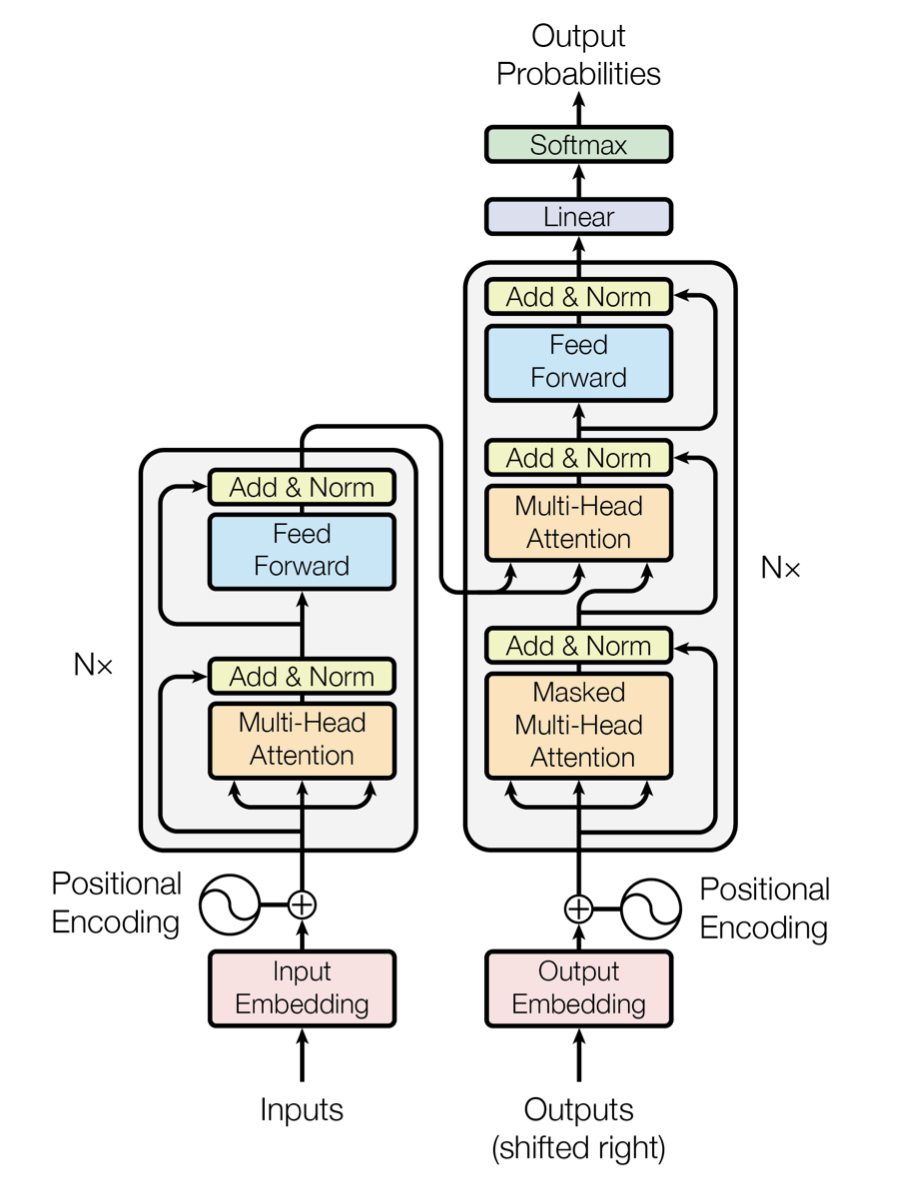
\includegraphics[width=0.5\textwidth]{figures/Transformer.png}
  \caption[Architecture of a Transformer model]{Architecture of a Transformer model. \cite{Vaswani2023}}
  \label{fig:transformer}
\end{figure}

These scores are referred to as logits, which are real-valued outputs representing the model’s raw, unnormalized preferences for each possible next token. Let $\mathbf{z} \in \mathbb{R}^n$ denote the vector of logits for all $n$ tokens in the vocabulary, where $z_i$ is the logit assigned to the $i$-th token and $z_j$ the logit for the $j$-th token. To convert these logits into a probability distribution over the vocabulary, the softmax function is applied. A temperature parameter $T$ can be used to control the randomness of the sampling process \cite{Peeperkorn2024}. The softmax function is defined as:
\begin{equation}
  \label{eq:softmax}
  \mathrm{softmax}(\mathbf{z})_i = \frac{\exp\left(\frac{z_i}{T}\right)}{\sum_{j=1}^{n} \exp\left(\frac{z_j}{T}\right)}.
\end{equation}

After applying the softmax function, the model obtains a probability distribution over the entire vocabulary. A decoding method then selects the next token from this distribution.

A common approach is stochastic sampling, where a token is drawn at random according to its probability in the distribution \cite{Brown2020}. The temperature parameter $T$ in Eq.~\eqref{eq:softmax} controls the sharpness of this distribution: $T < 1$ makes it more peaked, increasing the chance of selecting the most likely token, while $T > 1$ flattens it, making lower-probability tokens more likely. Setting $T = 0$ (interpreted as the limit $T \to 0$) effectively disables randomness, resulting in greedy decoding, where the token with the highest probability is always chosen \cite{Peeperkorn2024}.

State-of-the-art models such as OpenAI’s \ac{GPT} series or Meta’s \ac{LLaMA} family are decoder-only architectures that predict each token $t_i$ in an autoregressive manner \cite{Radford2018,Grattafiori2024}. These models are typically trained in an unsupervised fashion by maximizing the likelihood of the next token over large-scale text corpora. In earlier versions, such as GPT-1, fine-tuning on specific tasks was still necessary \cite{Radford2018}.

Subsequent research demonstrated that scaling model size and training data leads to emergent capabilities. \citet{Brown2020} showed that their 175-billion parameter model, \texttt{GPT-3}, could perform a variety of tasks without task-specific fine-tuning, using only \ac{ICL}. In this setting, the model receives task instructions and a few examples directly in the input prompt. For instance, to perform translation, the prompt might include \textit{house $\rightarrow$ Haus} and \textit{light bulb $\rightarrow$ Glühbirne}. Using one, several, or no examples is referred to as one-shot, few-shot, or zero-shot prompting, respectively.

\Ac{ICL} is particularly effective in large models because their greater parameter capacity allows them to capture more complex patterns and relationships from the training data. As a result, they can apply this knowledge to novel tasks with minimal guidance. Even without any examples in the prompt (zero-shot), models like \texttt{GPT-3} can achieve results that approach or, in some cases, match those of smaller models that have been fine-tuned for the task. To support such performance, \texttt{GPT-3} was trained on a filtered version of the Common Crawl corpus, along with other high-quality datasets, totaling over 500 billion tokens \cite{Brown2020}.

However, general web text corpora are not optimized for instruction-following tasks, and the original \texttt{GPT-3} was not fine-tuned to handle such prompts out of the box. \citet{Ouyang2022} point out that real-world usage often involves natural language instructions. To address this gap, they fine-tuned \texttt{GPT-3} using a two-step process. First, the model was trained on prompts paired with high-quality human-written completions. Second, human annotators ranked model outputs to train a reward model, which was then used in a reinforcement learning setup to further refine the base model.

The prompts for evaluation came from a held-out set of real user queries submitted to the \texttt{GPT-3} API. The resulting model, \texttt{InstructGPT}, achieved superior performance on these user-style prompts. Notably, even the smallest \texttt{InstructGPT} variant (1.3B parameters) outperformed the much larger base \texttt{GPT-3} (175B) in human evaluations, illustrating that instruction-fine-tuned models can be far more effective for instruction-based tasks than models trained purely to predict the next token in a sequence.

To evaluate and compare the performance of modern \acp{LLM}, a variety of benchmarks have been developed. One example is MMLU-Pro \cite{Wang2024}, which tests multitask language understanding across diverse domains such as mathematics, physics, law, and engineering. Another benchmark is the Chatbot Arena\footnote{Accessible at \url{https://lmarena.ai}}, a human preference evaluation platform where users compare the outputs of two models on the same prompt. From these comparisons, aggregated preferences are used to compute both a win rate and an overall ranking \cite{Chiang2024}.

The impressive performance of large models on these benchmarks is linked to their high complexity. Models such as \texttt{GPT-3}, with 175 billion parameters, require significant computational resources \cite{Brown2020,Frantar2023}. To make deployment more accessible, two main strategies are commonly pursued. The first is to use smaller models, often based on newer architectures that achieve prior state-of-the-art results with fewer parameters, thereby reducing computational demands while aiming to preserve accuracy \cite{Grattafiori2024,Meta2024}.

The second strategy is quantization, which compresses a model by reducing the bit-width used to store each parameter, thereby lowering memory requirements and increasing inference speed. Naive quantization often leads to large accuracy drops, so methods like GPTQ and AWQ introduce techniques to minimize this effect. GPTQ reduces quantization error during weight transformation, while AWQ preserves salient weights to maintain output quality. These techniques can achieve up to threefold speed-ups with minimal loss in performance compared to standard 16-bit precision \cite{Frantar2023,Lin2024}.

In conclusion, modern \acp{LM} are Transformer-based models that estimate the probability of the next token in a sequence. Their effectiveness is enabled by large-scale training, advanced architectural designs, and optimization techniques such as quantization. The evaluation of these models relies on benchmarks like MMLU-Pro and Chatbot Arena to assess their capabilities across diverse domains.

\section{Sentence Embeddings}
\label{sec:sentence_embeddings}

Sentence embeddings aim to represent textual input, such as full sentences or short passages, as dense vectors in a continuous vector space \cite{Singhal2001}. These vectors encode semantic information, allowing the similarity between different pieces of text to be measured mathematically. A common metric for this is cosine similarity, which computes the cosine of the angle between two vectors. A cosine similarity of 1.0 indicates identical direction (i.e., maximum similarity), while a value near 0.0 suggests minimal or no semantic similarity \cite{Singhal2001}. Figure~\ref{fig:cosine_similarity} illustrates how this measure reflects the angular relationship between two vectors.

\begin{figure}[t]
  \centering
  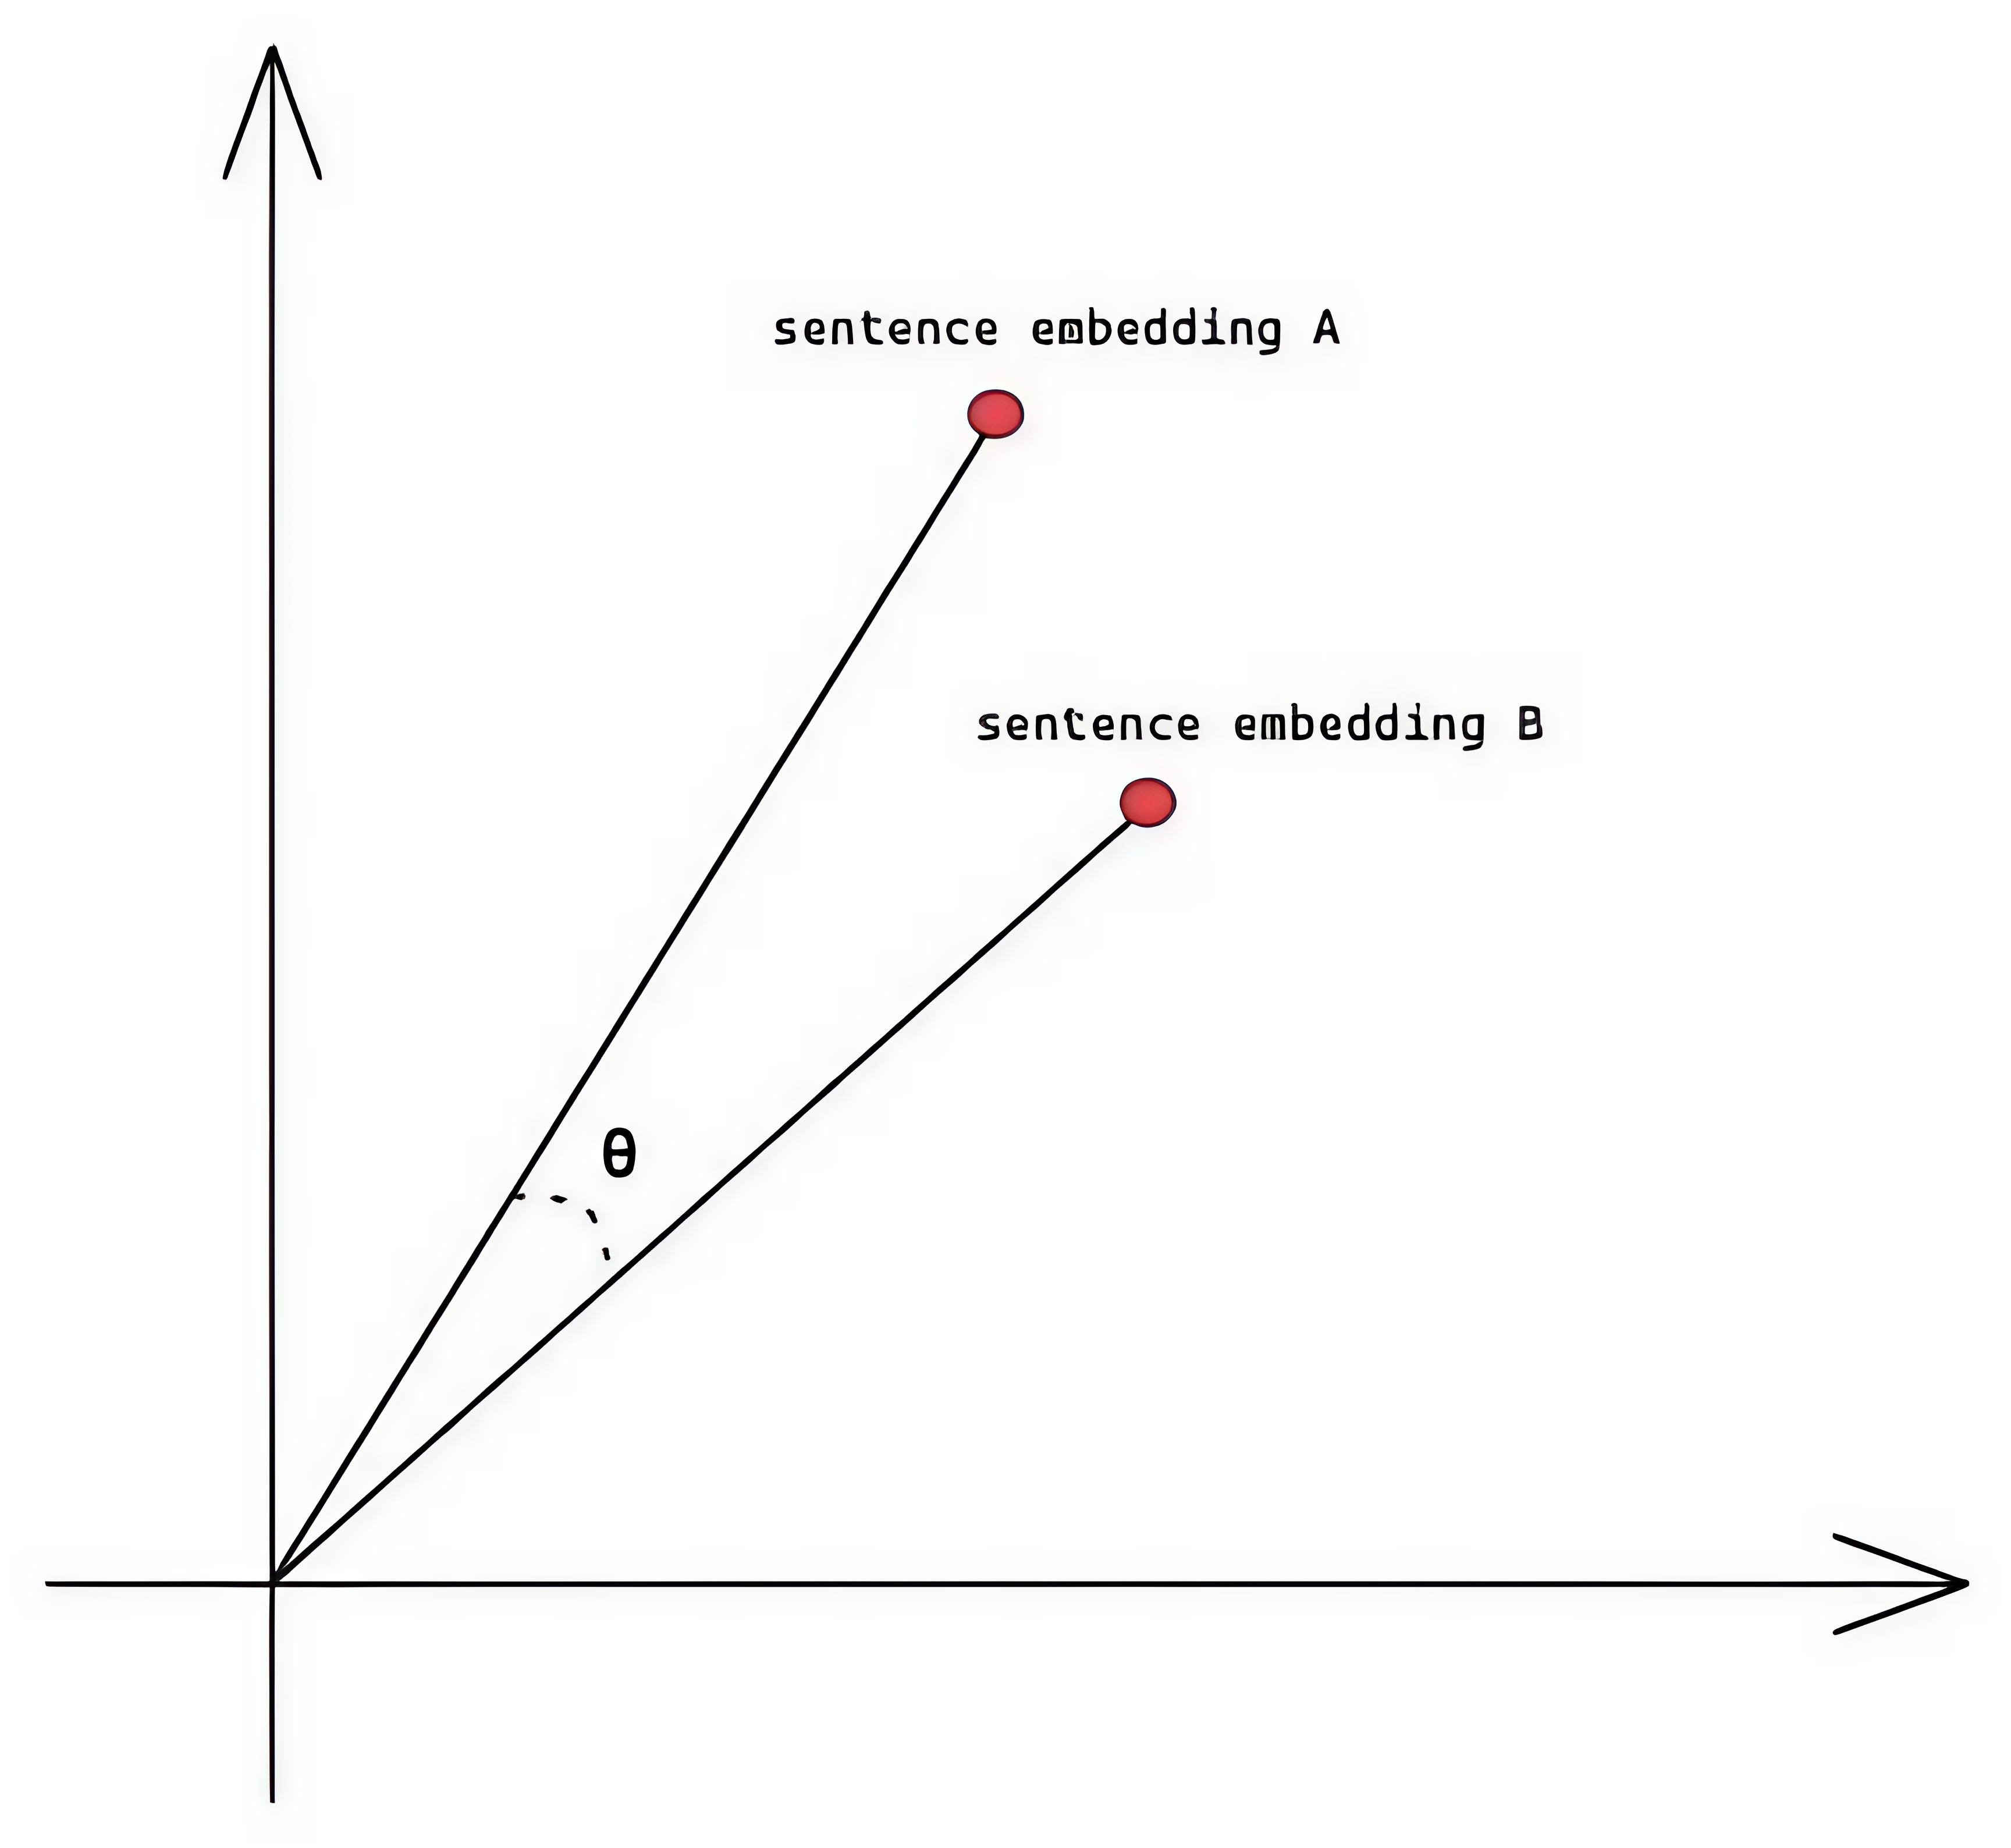
\includegraphics[width=0.6\textwidth]{figures/cosine_similarity.jpeg}
  \caption[Visualization of cosine similarity between two vectors showing how the angle between vectors determines their similarity score]{Visualization of cosine similarity between two vectors showing how the angle between vectors determines their similarity score. \cite{Leys2022}}
  \label{fig:cosine_similarity}
\end{figure}

Such embeddings are crucial for large-scale semantic similarity tasks, such as retrieving documents or knowledge passages relevant to a user query \cite{Reimers2019,Gao2024}. One recent approach is the M3-Embedding model, also referred to as \texttt{bge-m3}, which was developed to support multilingual and multi-purpose semantic retrieval across varying input granularities. To achieve this, it leverages the encoder architecture of Transformer-based models, as described in Section~\ref{sec:language_models} and illustrated in Figure~\ref{fig:transformer} \cite{Chen2024}.

According to \cite{Chen2024}, the training strategy for M3-Embedding follows a combination of pre-training and fine-tuning. During pre-training, the model was exposed to unlabeled corpora using weak semantic signals such as title–body or title–abstract pairs, and translation-based datasets were incorporated to support multilingual capabilities. Fine-tuning was performed using labeled data from multiple languages, as well as synthetic question–answer pairs generated by \texttt{GPT-3.5} from multilingual paragraphs. The model was optimized to determine whether a given query semantically matches a target passage, enabling it to perform robust retrieval across languages and domains \cite{Chen2024}.

To evaluate the performance of sentence embedding models across a wide range of downstream tasks, \citet{Muennighoff2023} introduced the \ac{MTEB} \footnote{available under \url{https://huggingface.co/spaces/mteb/leaderboard}}. \ac{MTEB} consists of 58 datasets covering diverse task categories such as classification, clustering, semantic textual similarity, reranking, retrieval, and summarization. It enables standardized comparisons between embedding models across languages, domains, and input types. Models such as M3-Embedding have achieved strong results on the \ac{MTEB} benchmark, particularly in multilingual retrieval and reranking tasks. This underlines \ac{MTEB}'s role as a comprehensive and practical framework for assessing the effectiveness of sentence embeddings across a wide range of real-world applications \cite{Muennighoff2023}.

In summary, sentence embeddings enable the representation of sentences in a vector space while preserving their semantic content. By applying vector operations such as cosine similarity, texts related to user queries can be identified efficiently. To achieve high performance on such tasks, recent embedding models like M3-Embedding combine Transformer-based architectures with large-scale pre-training and multilingual fine-tuning.


\section{Retrieval-Augmented Generation}
\label{sec:retrieval_augmented_generation}

As \acp{LM} are trained on static snapshots of large-scale corpora, they are inherently limited in their ability to access up-to-date or domain-specific information that lies outside their training data. \Ac{RAG} addresses this limitation by integrating external knowledge sources at inference time. In its simplest form, a \ac{RAG} system consists of three main components: indexing, retrieval, and generation \cite{Gao2024}.

In the indexing step, unstructured text documents are encoded into dense vector representations using embedding models such as M3-Embedding (see Section~\ref{sec:sentence_embeddings}) \cite{Gao2024}. These vectors are then stored in a vector database that supports efficient similarity search using vector algebra \cite{Gao2024,Pan2024}.

\begin{figure}[t]
  \centering
  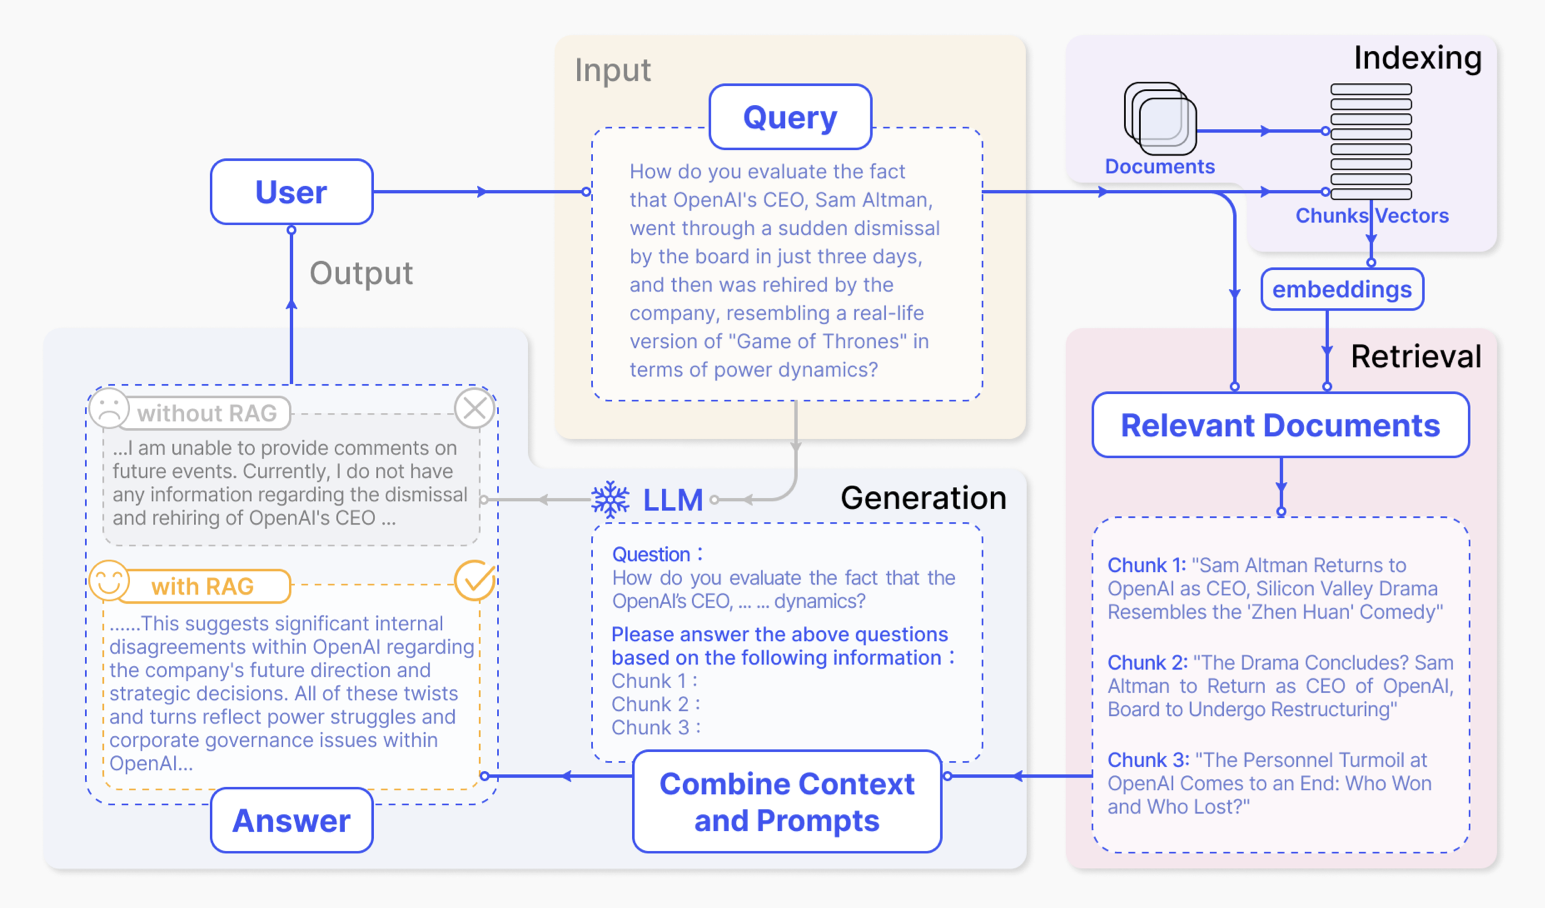
\includegraphics[width=0.8\textwidth]{figures/RAG.png}
  \caption[Overview of the Retrieval-Augmented Generation (RAG) architecture showing the indexing, retrieval, and generation pipeline]{Overview of the Retrieval-Augmented Generation (RAG) architecture showing the indexing, retrieval, and generation pipeline. \cite{Gao2024}}
  \label{fig:rag}
\end{figure}

Figure~\ref{fig:rag} illustrates the architecture of a typical RAG pipeline. While indexing is performed offline, the retrieval and generation steps occur at runtime. During retrieval, the user query is embedded into the same vector space using the same embedding model. Based on this embedding, a similarity search is performed on the vector database, retrieving the most relevant documents. The retrieved documents are then combined with the original user prompt and, if applicable, a system instruction to form the final prompt. The resulting prompt is passed to the \ac{LM}, which generates a response informed by the retrieved context \cite{Gao2024}.

A key component of the \ac{RAG} pipeline is the \ac{VDBMS}. Similar to traditional database systems, a \ac{VDBMS} comprises a query processor and a storage manager. The query processor handles vector-based similarity search and optimizes query execution. One example \ac{VDBMS} is Qdrant, which employs filtering strategies and adaptive execution paths depending on the size of the vector collection. For large collections, Qdrant reduces the search space through pre-filtering mechanisms, after which a brute-force search is performed on the remaining candidate vectors. The storage manager handles data persistence and access \cite{Pan2024,Qdrant2025}.

Qdrant organizes data into collections, which are logical groupings of vectors that often represent a specific domain or project. Each vector can be associated with metadata, called payloads, which support structured filtering during retrieval. The system provides integration with frameworks like Langchain, which facilitates the development of LLM-powered applications \cite{LangChain2025d}. Due to its optimization strategies, Qdrant enables efficient retrieval at scale even for large and complex datasets \cite{Pan2024,Qdrant2025}.

Despite its advantages, RAG systems are not without limitations. \citet{Barnett2024} identify several typical failure points in the RAG pipeline. These include cases where relevant information is missing from the indexed content, retrieved documents fail to rank highly enough to be included in the context, or documents are retrieved but discarded during context consolidation. Even when the relevant information is present, the language model may fail to extract it or ignore formatting constraints specified by the user \cite{Barnett2024}. Such issues highlight the importance of careful system design, particularly regarding retrieval accuracy, context management, and prompt construction.

In summary, \ac{RAG} provides a scalable and updatable mechanism for incorporating external knowledge into language model outputs. By combining dense semantic embeddings with similarity search in a \ac{VDBMS}, it enables the generation of context-aware responses grounded in up-to-date and domain-specific information.

\section{AI Agents}
\label{sec:ai_agents}

\citet{Dorri2018} defines an agent as \enquote{(a)n entity which is placed in an environment and senses different parameters that are used to make a decision based on the goal of the entity. The entity performs the necessary action on the environment based on this decision} \cite[S. 28574]{Dorri2018}. The environment describes the setting in which the agent operates and is shaped by factors such as data availability and quality, predictability of outcomes, the degree of change over time, and the continuity of the system state. Parameters refer to the data perceived by the agent, and actions are the set of operations it can perform in response \cite{Dorri2018}.

Agents typically operate based on a decision engine. In the case of \ac{AI} agents, this decision engine is commonly implemented using \acp{LLM} \cite{Sapkota2025,Park2023}. These agents are characterized by a high degree of independence, are tailored to specific tasks, and are capable of adapting their behavior to the current context \cite{Sapkota2025,OpenAI2025}. This distinguishes them from traditional workflow automation, where the sequence of steps is rigidly predefined \cite{Anthropic2024}. \acp{LLM} enable agents for human like behavior due to their internal representation of linguistic and behavioral patterns derived from large scale training corpora \cite{Park2023}.

An \ac{AI} agent system typically consists of three main components, namely an orchestration layer, a language model for decision making and reasoning, and a collection of external tools \cite{Wiesinger2025,OpenAI2025}. These components are coordinated by a runtime environment. The orchestration layer manages the agent’s memory, prepares prompt templates, and controls the message flow, thereby determining which information is passed to the agent and how the resulting actions are executed \cite{Wiesinger2025}.

According to \citet{OpenAI2025}, tools can be grouped into three categories: data tools, action tools, and orchestration tools. Data tools are designed to retrieve information from external systems, for example through database queries or web searches. Action tools allow agents to perform operations in external systems such as modifying records in a \ac{CRM}. Orchestration tools include other agents, enabling recursive structures which are further discussed in Section~\ref{sec:multi_agent_systems}. Tools enable agents to interact directly with their environment, thereby enhancing their autonomy and utility.

Each \ac{AI} agent is typically responsible for a clearly defined task and is equipped with a matching tool set. In such scenarios, \citet{Anthropic2024} suggest that an agent should be capable of processing complex inputs, using tools reliably, recovering from errors, and performing task level reasoning and planning. While this setup allows for independence within a task boundary, it limits flexibility beyond that scope unless multi agent orchestration is used \cite{Sapkota2025}.

One example of an \ac{AI} agent framework is ReAct, proposed by \citet{Yao2023}. ReAct combines stepwise reasoning and tool use by prompting the language model to alternate between generating thoughts and performing actions. This process allows agents to maintain a structured internal state composed of thoughts, actions, and observations. Based on this state, the model can iteratively reason about the next step and either call a tool, continue thinking, or terminate execution. The approach is motivated by the observation that human reasoning often interleaves mental reflection with real world interaction \cite{Yao2023}.

To build agents in practice, frameworks such as LangGraph are available. LangGraph is an open source framework for defining agent logic, memory, state tracking, and tool integration using either Python or JavaScript \cite{LangChain2025}. LangGraph supports high customizability and is part of the broader LangChain ecosystem. This ecosystem provides additional capabilities that are relevant for agent development, including direct LLM calling and tracing of execution flows \cite{LangChain2025a}.

While \ac{AI} agents provide a high degree of autonomy and adaptability, they are not without limitations. One key challenge lies in their limited ability to model causal relationships, as \acp{LLM} are primarily trained for next-token prediction rather than understanding cause and effect. Additionally, their performance is often highly dependent on the exact wording of the prompt, making outcomes less predictable. \citet{Sapkota2025} further note that current agents struggle with long-horizon planning in complex, multi-stage tasks, particularly when extended temporal consistency or contingency planning is required. Taken together, these issues can lead to failures in completing complex tasks reliably \cite{Sapkota2025}.


In summary, \ac{AI} agents are autonomous systems that make decisions using language models and interact with their environment through structured tools. They rely on orchestration mechanisms to manage memory and state. Frameworks such as ReAct illustrate one way to guide language model behavior in a controlled reasoning and action loop, but many architectures and implementations exist to serve different use cases.

\section{Multi-Agent Systems}
\label{sec:multi_agent_systems}

As stated in the previous section, agents are often limited to a single task, making them inflexible when addressing broader problems. A solution to this limitation can be found in \ac{MAS}. The idea is to develop a cost efficient, flexible and reliable system by using multiple agents instead of a single one. In this setup, a complex task can either be decomposed into multiple simpler tasks or the same task can be executed multiple times in parallel. The underlying theory is that such task distributions lead to more efficient solutions, which in turn compensates for the overhead associated with managing a \ac{MAS} \cite{Dorri2018}.

To make a general \ac{MAS} work, different agents are defined for specific subtasks. In some cases, several agents may handle the same task to increase redundancy or scalability. This requires a well-defined routing strategy within the \ac{MAS}, which can follow either a static or dynamic topology. In a static topology, a leader agent coordinates the other agents and serves as the central point of communication. In contrast, a leaderless \ac{MAS} allows each agent to decide autonomously which agent to invoke next \cite{Dorri2018}.

Leaderless systems introduce greater flexibility, but they also increase the complexity of coordination. Ensuring that all agents contribute effectively toward a shared goal becomes more challenging. Moreover, organizing inter-agent communication and assigning the correct tasks with appropriate inputs becomes increasingly difficult. Fault propagation and fault detection are also harder to manage when multiple agents contribute to a single outcome \cite{Dorri2018}.

These concepts can be extended to \ac{LLM}-based \acp{MAS}. Although single \ac{AI} agents powered by \acp{LLM} can already solve complex tasks, increasing complexity often leads to failure modes such as looping or tool misuse (see Section~\ref{sec:ai_agents}) \cite{OpenAI2025}. Therefore, decomposing goals into smaller subtasks managed by specialized agents can be beneficial \cite{Sapkota2025}.

Each \ac{LLM}-based agent generally shares the same architectural components discussed in Section~\ref{sec:ai_agents}. In a \ac{MAS}, however, these components are further extended. In particular, the agent state is transformed into a shared state accessible across agents \cite{Sapkota2025}. Each agent must also define a handoff mechanism, which determines the next tool or agent to invoke and the corresponding input or state update. In frameworks like LangGraph, handoffs specify the destination and include a payload that updates the shared state. This shared state is typically implemented as a Python dictionary with predefined fields. Consequently, the orchestration layer becomes more complex, and this complexity is managed by agent frameworks like LangGraph \cite{LangChain2025b}.

\begin{figure}[t]
  \centering
  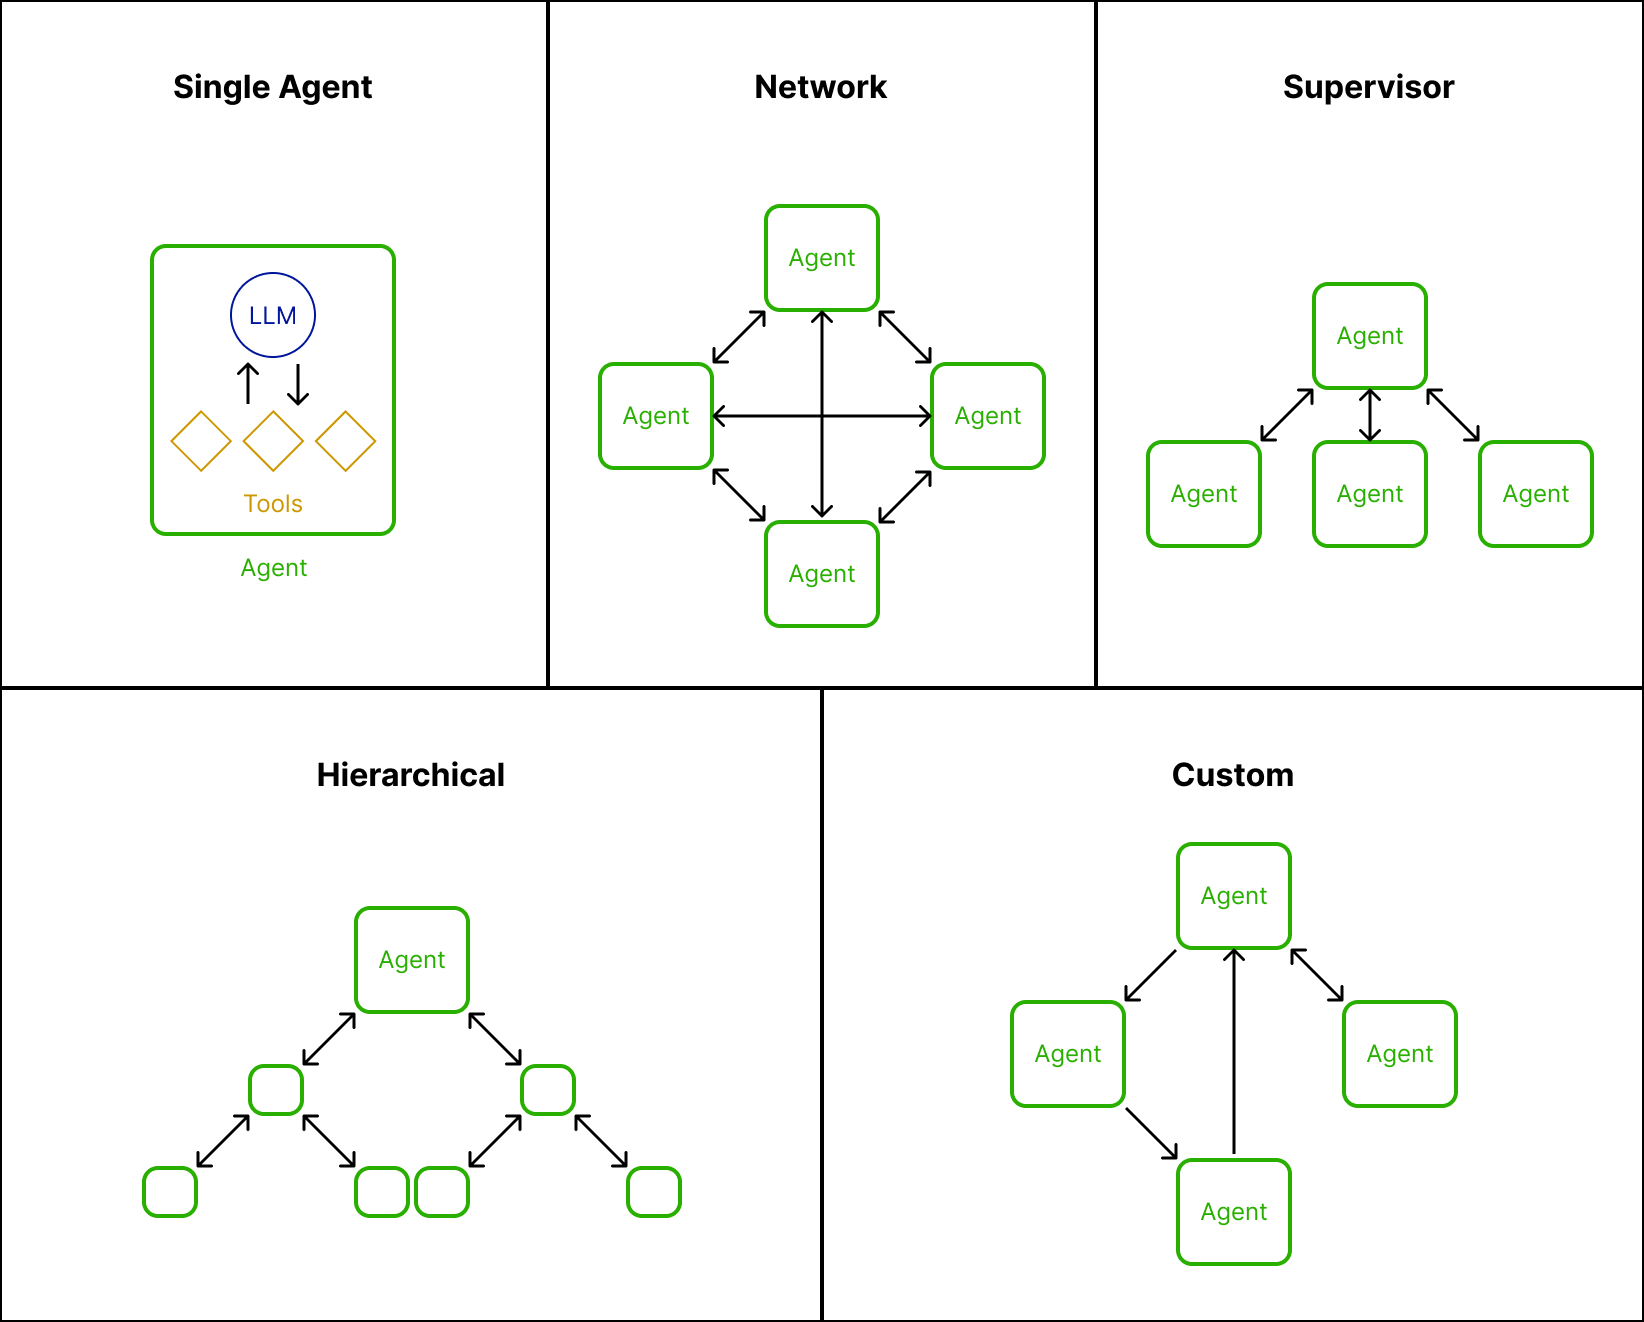
\includegraphics[width=0.8\textwidth]{figures/Multi-agent architectures.png}
  \caption[Example multi-agent architecture patterns showing supervisor, hierarchical, network, and custom patterns for LLM-based \acp{MAS}]{Example multi-agent architecture patterns showing supervisor, hierarchical, network, and custom patterns for LLM-based \acp{MAS} (self-created after \cite{LangChain2025b})}
  \label{fig:mas_architecture}
\end{figure}

\citet{LangChain2025b} describe several agentic architecture patterns for \ac{LLM}-based \acp{MAS}, which follow classic \ac{MAS} designs (see Figure~\ref{fig:mas_architecture}). The supervisor pattern represents a leader-follow structure in which a central supervisor agent coordinates the communication with specialized expert agents. These expert agents do not communicate with each other, but only with the supervisor. The hierarchical pattern extends this idea by allowing expert agents to act as intermediate supervisors themselves, enabling a multi-level structure with distributed decision-making responsibilities \cite{LangChain2025b}.

\ac{LLM}-based \acp{MAS} can also follow decentralized, leaderless designs \cite{OpenAI2025,LangChain2025b}. In the network pattern, each agent decides independently which other agent to pass control to, effectively managing the process flow itself \cite{LangChain2025b,OpenAI2025}.

Custom patterns, as described by \citet{LangChain2025b}, do not strictly belong to either leaderless designs or supervisor-based patterns. They enable bespoke configurations, such as limiting communication between specific agents or implementing fixed workflows. Such designs enable highly individualized and adaptable agent roles, particularly when implemented with frameworks like LangGraph \cite{LangChain2025b}.

Despite their advantages, \ac{LLM}-based \acp{MAS} also introduce new challenges. First, the lack of causal reasoning in \acp{LLM} becomes more problematic as agents must interact multiple times. Each \ac{AI} agent already introduces uncertainty due to prompt sensitivity and a tendency to enter infinite loops. Using multiple agents compounds this uncertainty and increases the overall system fragility \cite{Sapkota2025}. Furthermore, coordinating communication between agents exposes additional bottlenecks, particularly given the limited context windows of \acp{LLM}, both model-wise and infrastructure-wise \cite{Kwon2023}. Maintaining a shared context and ensuring alignment across agents becomes increasingly difficult \cite{Sapkota2025,Han2025}.

Another critical issue is non-composability. Because \acp{LLM} may respond unpredictably, introducing a new agent into the system does not guarantee that it will be utilized effectively. Instead, it may increase prompt complexity without improving performance. As the number of agents grows, tracing the source of errors also becomes harder due to the sensitivity of \acp{LLM} to prompt changes. In addition, the field of \ac{LLM}-based \acp{MAS} remains relatively immature, which contributes to the lack of standardized solutions \cite{Sapkota2025}.

Nonetheless, recent work has begun to address some of these problems. For instance, integrating retrieval-augmented generation can help mitigate reasoning gaps by supplying agents with relevant external knowledge. The use of deterministic tools within the agent loop also improves reliability. Monitoring and auditing tools can support root cause analysis, and simulation tools may enhance causal awareness. Communication challenges may be addressed through improved memory architectures and coordination mechanisms \cite{Sapkota2025}.

In summary, \ac{LLM}-based \acp{MAS} offer a promising approach to solving complex problems through the collaboration of multiple specialized \ac{AI} agents. These systems can be organized hierarchically, networked, or in fully custom configurations. While they provide flexibility and scalability, they also introduce challenges such as error amplification, coordination overhead and reduced traceability. As research in this area progresses, new techniques and tools continue to emerge to address these limitations and improve the robustness of such systems.

\section{AI Agent Design}
\label{sec:agent_design}

As the field of \ac{AI} agent research matures, so does the understanding of when and how to use such agents effectively. In general, \citet{OpenAI2025} recommend employing \ac{AI} agents when deterministic rules fall short, particularly when the problem cannot be easily formalized into a ruleset. This is especially true in cases involving complex decision-making or unstructured data, where \ac{AI} agents are likely to outperform rule-based systems \cite{OpenAI2025}.

As described in Section~\ref{sec:ai_agents}, \ac{AI} agents are typically designed for a single task and constrained by the context they can process. These limitations become apparent when agents begin to fail at following instructions or when their decision-making performance degrades. Some problems are inherently too complex in terms of context or tool usage, leading to tool overload. In such cases, task and tool responsibilities can be decomposed across a \ac{MAS}. This approach is particularly useful when problems require complex logic that benefits from being broken into subtasks \cite{OpenAI2025,LangChain2025b}. However, \ac{LLM}-based \acp{MAS} should be used thoughtfully, as their architecture entails high cost and complexity \cite{Hadfield2025}.

Regarding agent design, \citet{Anthropic2024} emphasize prioritizing simplicity over complexity. They argue that agentic systems should strike a balance between latency and task performance. Similarly, \citet{Hadfield2025} propose treating agent systems like human teams. Tasks should be concise, actions clearly defined, and the context understandable to humans, given that \acp{LLM} are trained on human-generated text. Context compression is another recommended technique to keep prompts manageable and more interpretable \cite{Hadfield2025}. These principles support the hypothesis proposed by \citet{Anthropic2024}, which suggests that if a human can solve a task, an \ac{AI} agent should be able to solve it as well, provided the problem is stated clearly. Aligned with these principles, \citet{OpenAI2025} advise capturing edge cases early to improve agent robustness and keeping components modular and composable, particularly in \ac{LLM}-based \acp{MAS}.

Since \acp{LLM} remain prompt-sensitive, effective prompt engineering is essential. \citet{Anthropic2024} suggest considering the training background of the model. As \acp{LLM} are primarily trained on prose and optimized to generate coherent text, prompts should closely resemble the structure and format of natural language. Unnecessary formatting should be avoided, as it may reduce performance. Furthermore, \citet{Hadfield2025} recommend teaching agents how to orchestrate the \ac{MAS}, including a guided reasoning process. Overall, prompt clarity and structure are key to agent effectiveness \cite{OpenAI2025}.

As outlined in Section~\ref{sec:language_models}, one effective prompting strategy is \ac{ICL}. When applying one-shot or few-shot prompting, decisions must be made regarding the number, order, format, and similarity of the examples \cite{Schulhoff2025}. Various prompting styles such as role prompting, style prompting, or emotion prompting can also influence outcomes. Another popular method is \ac{CoT} prompting, which encourages the model to reason step by step. Few-shot \ac{CoT} extends this by incorporating worked-out examples, such as complete reasoning traces leading to correct answers. Automatic prompt optimization can further improve agent performance \cite{Schulhoff2025}.

\citet{Schulhoff2025} evaluate various prompting strategies using the MMLU benchmark, which is closely related to the MMLU-Pro benchmark discussed in Section~\ref{sec:language_models}. Their findings show that few-shot \ac{CoT} prompting performed best, while zero-shot \ac{CoT} performed worst. These results align with earlier findings by \citet{Brown2020}, who described \acp{LM} as effective few-shot learners.

In addition to prompt engineering, well-designed tools are crucial for tasks requiring interaction with external systems or knowledge \cite{OpenAI2025,Anthropic2024}. According to \citet{Anthropic2024}, tool descriptions must be as carefully engineered as the prompts themselves. \acp{LLM} must be able to generate structured handoffs from unstructured input based on the tool descriptions. Tools should be tested thoroughly, and their usage logged for traceability. Making tools foolproof can reduce the likelihood of errors and support more robust performance \cite{Anthropic2024}.

Once agents are deployed, performance iteration is key. \citet{Hadfield2025} recommend beginning evaluation with small examples and incorporating human oversight to identify errors not easily caught through automation. In particular, tool execution should be traced and debugged to identify weak points. One example of a platform for this kind of engineering is Langfuse \cite{LGFT2025}.

In summary, given the limitations of \acp{LLM}, careful agent design is essential. Effective \ac{AI} agents and \ac{LLM}-based \acp{MAS} must be modeled after human problem-solving processes and supported through robust prompt and tool engineering. When well designed, such systems can effectively address complex tasks \cite{Hadfield2025}.

\chapter{Related Work}
\label{ch:related_work_chapter}

This chapter presents the current state-of-the-art training and benchmarking datasets as well as various approaches in the field of information extraction, with a particular focus on solutions in the area of \ac{cIE}. Section~\ref{sec:related_datasets} discusses the REBEL dataset, one of the first large-scale datasets for open and closed information extraction, followed by the synthIE dataset, a synthetically generated resource based on models from the \texttt{GPT-3.5} family. Section~\ref{sec:related_approaches} outlines different methodological approaches, ranging from transformer fine-tuning and prompt tuning to the use of \ac{AI} agents for open and closed information extraction.

\section{Related Datasets}
\label{sec:related_datasets}

Datasets are crucial for training, and especially for evaluating, approaches in the domain of \ac{cIE}. This requires not only high-quality but also large-scale datasets \cite{Josifoski2023}. The REBEL dataset was created by analyzing Wikipedia abstracts and extracting all hyperlinks. Additionally, a \texttt{RoBERTa}-based \ac{LM} was used to filter whether a text entails the extracted triples by leveraging \texttt{RoBERTa}’s entailment prediction capabilities. This results in a large-scale, automatically created dataset in which noise is accepted. Accordingly, the REBEL dataset can be classified as a silver-standard dataset. Such datasets typically contain a higher level of noise and lower reliability compared to human-annotated (gold-standard) datasets \cite{HuguetCabot2021}\footnote{The REBEL dataset is publicly available on Hugging Face: \url{https://huggingface.co/datasets/Babelscape/rebel-dataset}}.

To address issues with noise and predicate frequency skewness in the REBEL dataset, \citet{Josifoski2023} introduced the synthIE dataset. The idea is to leverage the text generation capabilities of \acp{LLM} from the \texttt{GPT-3.5} series to generate texts that correlate with expected triples \cite{Josifoski2023}. \citet{Josifoski2023} created an unskewed set of triples based on a subset of Wikidata and prompted these with corresponding instructions into \texttt{text-davinci-003}, which produced the dataset \texttt{synthIE-text}, or \texttt{code-davinci-002}, a base \texttt{GPT-3.5} model that produced the dataset \texttt{synthIE-code} \cite{Josifoski2023,OpenAI2025a}. Human-annotated samples revealed that, in contrast to the REBEL dataset, most of the triples within the generated texts of the synthIE dataset were detectable \cite{Josifoski2023}\footnote{The dataset is publicly available on Hugging Face: \url{https://huggingface.co/datasets/martinjosifoski/SynthIE}}.

Both the REBEL dataset and the synthIE dataset provide pairs of natural language text and corresponding knowledge triples. These triples include not only the surface forms of entities and predicates as they appear in the text, but also an identifier for the corresponding entry in Wikidata. This enables evaluation for \ac{cIE} approaches on both datasets.

In practical evaluation scenarios, however, the REBEL dataset has shown significant limitations. Many of the provided triples represent only a fraction of the relations that are actually present in the input text. For example, in the sentence \enquote{Richard H. Weisberg is a professor of constitutional law at the Cardozo School of Law at Yeshiva University in New York City, a leading scholar on law and literature}, the expected triples are limited to \textit{(Cardozo School of Law; headquarters location; New York City)} and \textit{(Yeshiva University; located in the administrative territorial entity; New York City)}. Other relevant facts such as \textit{profession}, \textit{employer}, or \textit{field of work} are not included, despite being inferable from the text.

Furthermore, a notable portion of the documents in the REBEL dataset spans multiple paragraphs, which increases the complexity of \ac{cIE} without offering a proportional benefit in evaluation quality. Combined with the reduced coverage of semantically relevant information, these issues significantly impair the usefulness of the REBEL dataset as a benchmark for evaluating system performance. As a result, subsequent development and evaluation in this work primarily rely on the higher-quality synthIE dataset.

In summary, \citet{HuguetCabot2021} and \citet{Josifoski2023} provided large-scale datasets. The synthIE dataset is of higher quality and thus yields better results when used for evaluation. Both the REBEL dataset and the synthIE dataset offer extensive training, validation, and test splits, serving as a foundation for the development of approaches in \ac{cIE}.

\section{Related Approaches}
\label{sec:related_approaches}

As outlined in Section~\ref{sec:closed_information_extraction}, open and closed information extraction methods follow either pipeline or joint approaches. These rely on a broad variety of techniques, ranging from probability learning approaches to LSTM-based models and encoder-decoder architectures \cite{Zhang2022,Angeli2015,Trisedya2019}. With the rise of Transformer-based architectures, recent approaches predominantly implement Transformer models \cite{Josifoski2021,Josifoski2023,Moeller2024}.

Even before the emergence of \acp{LLM}, Transformer models demonstrated superior performance compared to other state-of-the-art methods. A prominent example is the REBEL model trained on the REBEL dataset \cite{HuguetCabot2021}. By fine-tuning a \texttt{BERT} \ac{LM} with texts as input and triples as output, \citet{HuguetCabot2021} achieved superior results on benchmarking datasets, presenting a flexible relation extraction model.

\citet{Josifoski2021} introduced GenIE, adapting the REBEL framework for \ac{cIE}. In their approach, \citet{Josifoski2021} constrained the decoding process in the \texttt{BART}-based \ac{LM} so that it would generate only outputs aligned with entities and relations from the underlying knowledge base Wikidata. They applied output linearization by introducing special tokens to delimit subject, predicate, and object. Furthermore, a constrained beam search was implemented to ensure that only valid tokens from Wikidata could be generated. This method outperformed a traditional pipeline consisting of named entity recognition, entity disambiguation, relation classification, and triplet classification \cite{Josifoski2021}.

Building upon GenIE and the quality of the synthIE dataset, \citet{Josifoski2023} proposed the synthIE model. While following GenIE’s architecture, the synthIE model replaces \texttt{BART} with \texttt{Flan-T5} due to broader availability of pre-trained configurations. The best-performing synthIE model, trained on the training split of the synthIE dataset, surpassed a Flan-T5-based GenIE variant trained on the REBEL dataset by over 0.8~macro-$F_{1}$ on the \texttt{synthIE-text} test set. This result highlights the strong correlation between the quality of training and benchmarking datasets and overall model performance \cite{Josifoski2023}.

Exploring foundation models that can be fine-tuned or prompt-engineered, \citet{Xue2024} proposed a pipeline approach using fine-tuned \acp{LLM} for relation extraction, subject identification, and triplet fact extraction. In contrast, \citet{Chen2024} introduced a prompt-tuning method for joint optimization. The approach by \citet{Xue2024} achieved a 10\% F1-score improvement on the document-level open information extraction dataset Re-DocRED compared to prior models. Moreover, they demonstrated that base models like ChatGPT were clearly outperformed by fine-tuned models \cite{Xue2024}.

\citet{Chen2024}, on the other hand, applied prompt tuning for open information extraction across sentence boundaries rather than full documents. Their results showed that well-designed prompt tuning strategies can match the performance of fine-tuned approaches. \citet{Chen2024} did not compare their model to other approaches presented in this work. It should be noted that both \citet{Chen2024} and \citet{Xue2024} used datasets focused on open information extraction rather than \ac{cIE}. As a result, their performance metrics are not directly comparable to approaches evaluated on the REBEL dataset or the synthIE dataset. In general, comparing models trained and tested on different datasets provides limited insight into their relative strengths, particularly in task-specific contexts like \ac{cIE}.

The most similar approach to this work is AgentRE by \citet{Shi2024}. Leveraging advances in AI agents, they proposed a single-agent framework for open information extraction. In their design, the agent had access to both a retrieval module and a memory module. The retrieval module provided relevant samples and context from a knowledge graph, including sample triples and relation descriptions. Meanwhile, the memory module stored correct and incorrect extractions and supported self-reflection with the help of the \ac{LLM}. By orchestrating these components, the agent was able to extract valid triples from input texts \cite{Shi2024}.

AgentRE was evaluated on several benchmark datasets unrelated to the REBEL dataset or the synthIE dataset. The main dataset, SciERC, is limited and outdated \cite{Luan2018}. Experiments using \texttt{GPT-3.5 Turbo} and a reasoning-enhanced \texttt{LLaMA-2-7B} model showed that AgentRE outperformed other methods on most of the datasets evaluated by \citet{Shi2024}, highlighting the potential of AI agents for information extraction \cite{Shi2024}. However, as with other approaches, the implications for \ac{cIE} remain limited.

In summary, recent advances in \ac{LLM} research have demonstrated improvements in both open and closed information extraction. A range of approaches such as fine tuning, prompt tuning, and agent based frameworks can address the problem. Furthermore, the importance of high quality datasets for training and especially for benchmarking in \ac{cIE} has been clearly demonstrated. However, many of the approaches discussed either do not use the latest \acp{LLM} or do not directly address \ac{cIE}, and closed information extraction has so far relied mainly on fine tuned Transformer models that require large training datasets. While large language models have been applied to open information extraction, their use in closed information extraction and the integration of artificial intelligence agents in this domain remain unexplored.

\chapter{Approach}
\label{ch:approach}

This work introduces CIExMAS, a novel approach to \ac{cIE} based on \acp{MAS}. The core idea is to evaluate both the pipeline and the joint approach to \ac{cIE} through multiple specialized agents. To fulfil this task, agents must be capable of accessing and retrieving data directly from the knowledge graph. For this reason, the concept of tools is employed.

Instead of relying on model fine tuning, the proposed \ac{MAS} is designed entirely around prompt tuning and \ac{ICL}. The overarching goal is to create a system that can be applied in real world scenarios. In this context, real world applicability means that the system must be able to handle diverse text types and operate with different knowledge graphs. The decision to focus on \ac{ICL} is informed by findings from \citet{Brown2020}, who showed that, within the \texttt{GPT-3} language model, this method could be used effectively and, in certain cases, even surpass domain specific fine tuned models. Moreover, recent advancements in large language models demonstrate that newer architectures can match or surpass the performance of their predecessors, sometimes with fewer parameters \cite{MetaAI2025,Chiang2024}. Details on the language models used in this work are provided in Section~\ref{subsec:eval_language_models}.

An iterative development process was followed to design and evaluate a range of \acp{MAS}, drawing on the best practices discussed in Section~\ref{sec:agent_design}. To the best of the author's knowledge, no prior research has proposed a \ac{MAS} specifically for \ac{cIE}, which made the iterative process essential as it enabled the identification of limitations in early designs and informed subsequent refinements. As a result, five core architectures emerged.

The \textit{baseline architecture}, described in Section~\ref{subsec:baseline}, follows a strict pipeline-oriented design. The \textit{\ac{SSA}} and \textit{\ac{SSSA}} architectures, outlined in Sections~\ref{subsec:supervisor} and~\ref{subsec:simplified_splitted_supervisor}, introduce task-splitting mechanisms based on the baseline. In contrast, the \textit{ReAct architecture} in Section~\ref{subsec:react} simplifies the system by consolidating all responsibilities into a single agent while retaining tool usage. Finally, the \textit{network architecture}, detailed in Section~\ref{subsec:network}, demonstrates how expert agents can autonomously define and manage the system's flow.

In addition to agent structures, several tools were developed. The most important tool for \ac{cIE} is the \textit{\ac{URI} retrieval tool} (Section~\ref{subsec:uri_retrieval}), which performs a similarity search to support the mapping of search terms to corresponding \acp{URI}. To further increase knowledge graph integration, additional tools were designed, including the \textit{network traversal tool} (Section~\ref{subsec:network_traversal}), the \textit{semantic validation tool} (Section~\ref{subsec:semantic_validation}), and the \textit{turtle-to-label tool} (Section~\ref{subsec:turtle_to_label}). However, the presence of a tool does not imply that it was integrated into every architecture.

Agents are implemented as calls to \acp{LLM} using a prompt template, which is dynamically filled with selected input fields. In principle, many \acp{LLM} supported in LangChain offer structured output parsing, where responses can be automatically mapped to predefined schemas \cite{LangChain2025e}. Since this functionality was not consistently supported across all used models, this work instead relies on parsing structured data directly from the model-generated text. To enable this, the \ac{LLM} is instructed to output specific XML tags containing information about the next agent, the final output, instructions for subsequent agents, or the input for tools.

It is important to note that all architectures were iteratively refined with regard to prompt design and tool usage, especially those that demonstrated promising results. As previously mentioned, the development of tools was driven by the iterative process chosen for this work. Consequently, certain tools were designed exclusively for specific architectures. Details on which tools were used with which configurations are provided in Section~\ref{sec:evaluation_configurations}.

\section{Agent Architectures}
\label{sec:agent_architectures}

This section presents the different agent architectures developed in this work. Each architecture is described with respect to the specific agents involved, the overall system flow, and the processes for transferring control or data between agents. Furthermore, the definition of agent state and the process of passing control or data from one agent to another are outlined for each architecture. Understanding these architectural variations is essential for evaluating the trade-offs between modularity, control, and performance in \acp{MAS} for \ac{cIE}.

\subsection{Baseline Architecture}
\label{subsec:baseline}

\begin{figure}[tp]
  \centering
  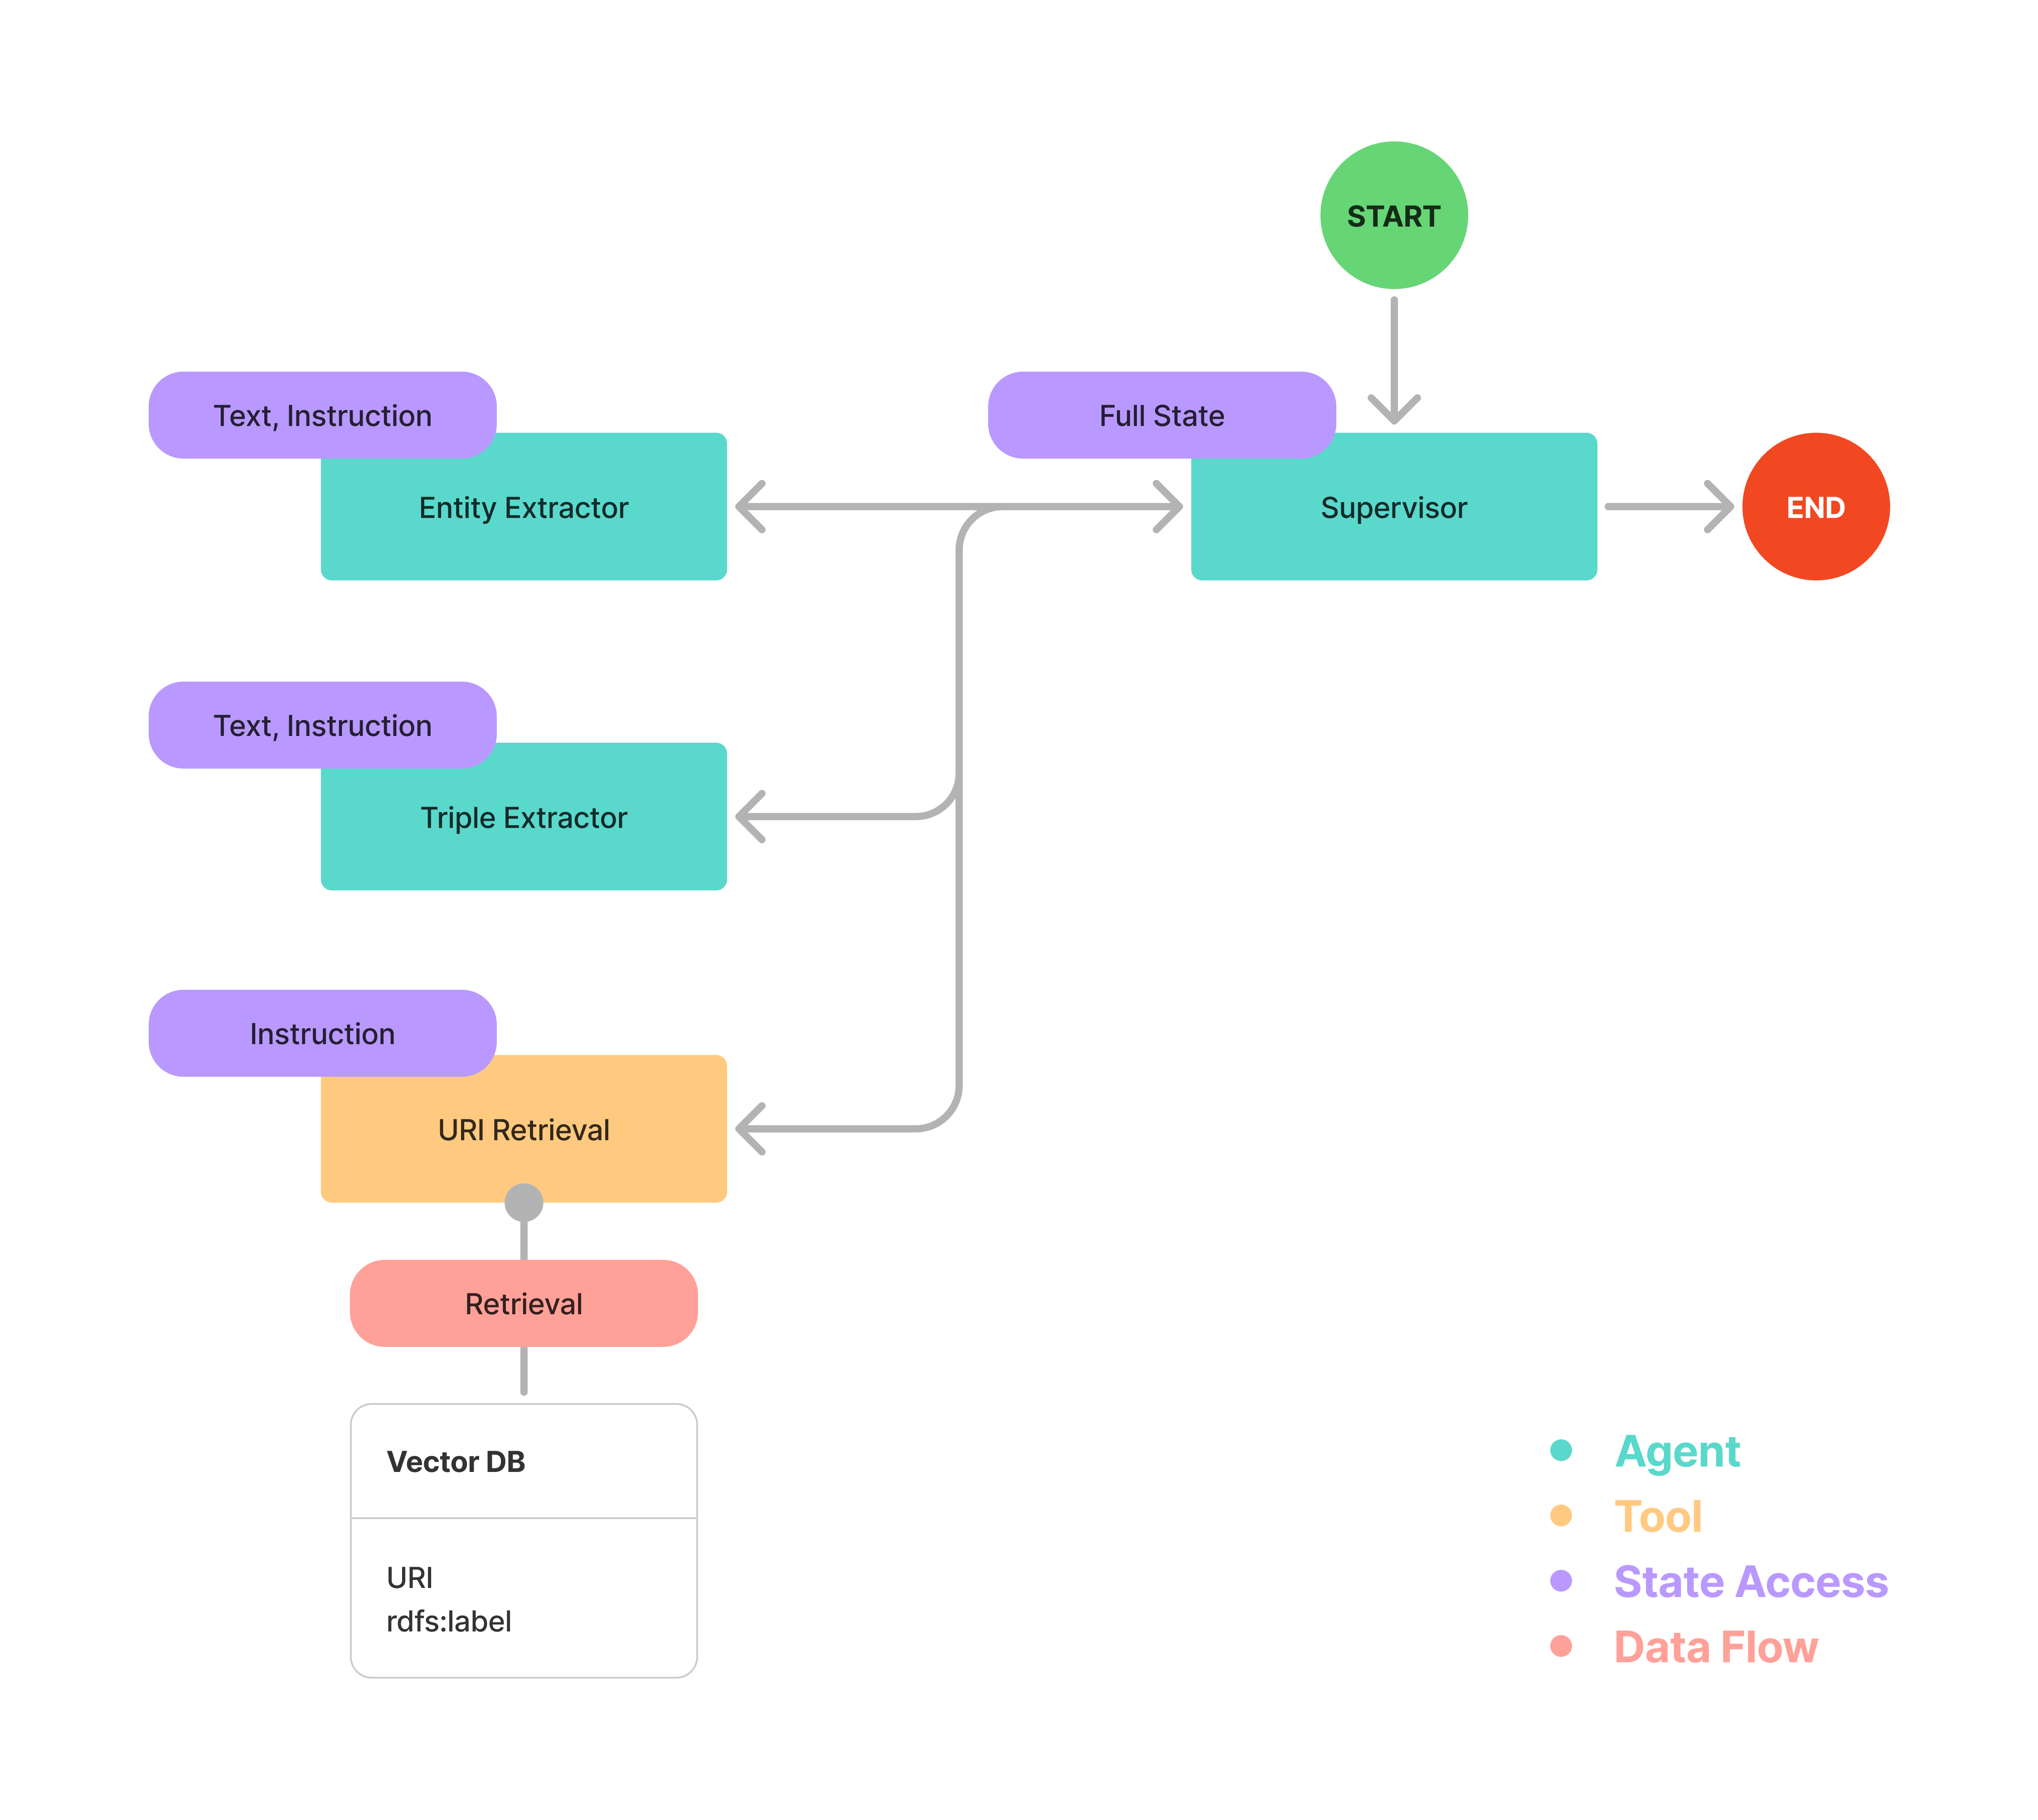
\includegraphics[width=0.7\textwidth]{figures/Baseline Architecture.png}
  \caption[Baseline architecture showing the pipeline approach with specialized agents for each step of the closed information extraction process]{Baseline architecture showing the pipeline approach with specialized agents for each step of the closed information extraction process (self-created)}
  \label{fig:baseline_architecture}
\end{figure}

The \textit{baseline architecture} represents the initial implementation of a \ac{MAS} for closed information extraction in this work. It follows a classical pipeline approach to \ac{cIE} by introducing two specialized agents: an \textit{entity extractor} and a \textit{triple extractor}. This reflects the multi-agent principle of decomposing complex tasks. Closed information extraction is commonly considered such a task \cite{Josifoski2021}. Additionally, the architecture implements a \textit{supervisor} agent that aligns with the supervisor pattern and coordinates the workflow and communication between agents. In this configuration, the \textit{\ac{URI} retrieval tool} is already integrated to map the free-text triples to corresponding \acp{URI}. An overview of this architecture is shown in Figure~\ref{fig:baseline_architecture}.

At the core of the \textit{baseline architecture} lies the concept of state, represented as a dictionary containing key information exchanged between agents and tools. Table~\ref{tab:baseline_state} summarizes its main fields.

\begin{table}[h]
  \centering
  \caption{State fields in the \textit{baseline architecture}}
  \label{tab:baseline_state}
  \begin{tabular}{p{3cm}p{10cm}}
    \toprule
    \textbf{Name}        & \textbf{Description}                                                                \\
    \midrule
    \texttt{text}        & The document or sentence being processed.                                           \\
    \texttt{messages}    & List of exchanged messages between agents, enabling history tracking and reasoning. \\
    \texttt{instruction} & Task-specific instructions for agents or tools.                                     \\
    \bottomrule
  \end{tabular}
\end{table}

Because this is a supervisor-based architecture, orchestration and routing are fully managed by the \textit{supervisor agent}. It is the only agent with access to the complete system state. In addition to coordinating the sequence of operations, the \textit{supervisor agent} is responsible for validating intermediate results and formatting the final output. After invoking the specialized agents for \textit{entity extraction} and \textit{triple extraction}, the \textit{supervisor agent} assesses the quality of the returned results. If needed, it can initiate additional reasoning steps or repeat certain parts of the process. This includes re-running agents to improve disambiguation. The \textit{supervisor agent} uses the \texttt{instruction} field to send specific prompt inputs to other agents and tools. When a triple is produced by the \textit{triple extractor}, the \textit{supervisor agent} constructs search terms and queries the \textit{\ac{URI} retrieval tool}. Based on the retrieved \acp{URI}, the \textit{supervisor agent} composes a valid \texttt{Turtle} output.

The \textit{entity} and \textit{triple extraction agents} are entirely based on prompt engineering. Initially, both agents were prompted with simple instructions requesting entity or triple extraction respectively. Over the course of the iterations, these agents are expected to perform increasingly well on their narrow tasks as prompts are refined iteratively. Details about the overall prompt engineering process are described in Section~\ref{sec:iterative_prompt_engineering}.

Overall, this baseline design results in a pipeline, in case any result is error-free. First, entities are extracted. Then, triples are constructed. The supervisor retrieves matching \acp{URI} and generates a final \texttt{Turtle} output. If this process fails, for example due to missing or incorrect entities or predicates, the supervisor can repeat parts of the workflow. This flexibility allows the architecture to extend beyond a purely linear structure and reduces the risk of error propagation.

\subsection{Splitted Supervisor Architecture}
\label{subsec:supervisor}

\begin{figure}[tp]
  \centering
  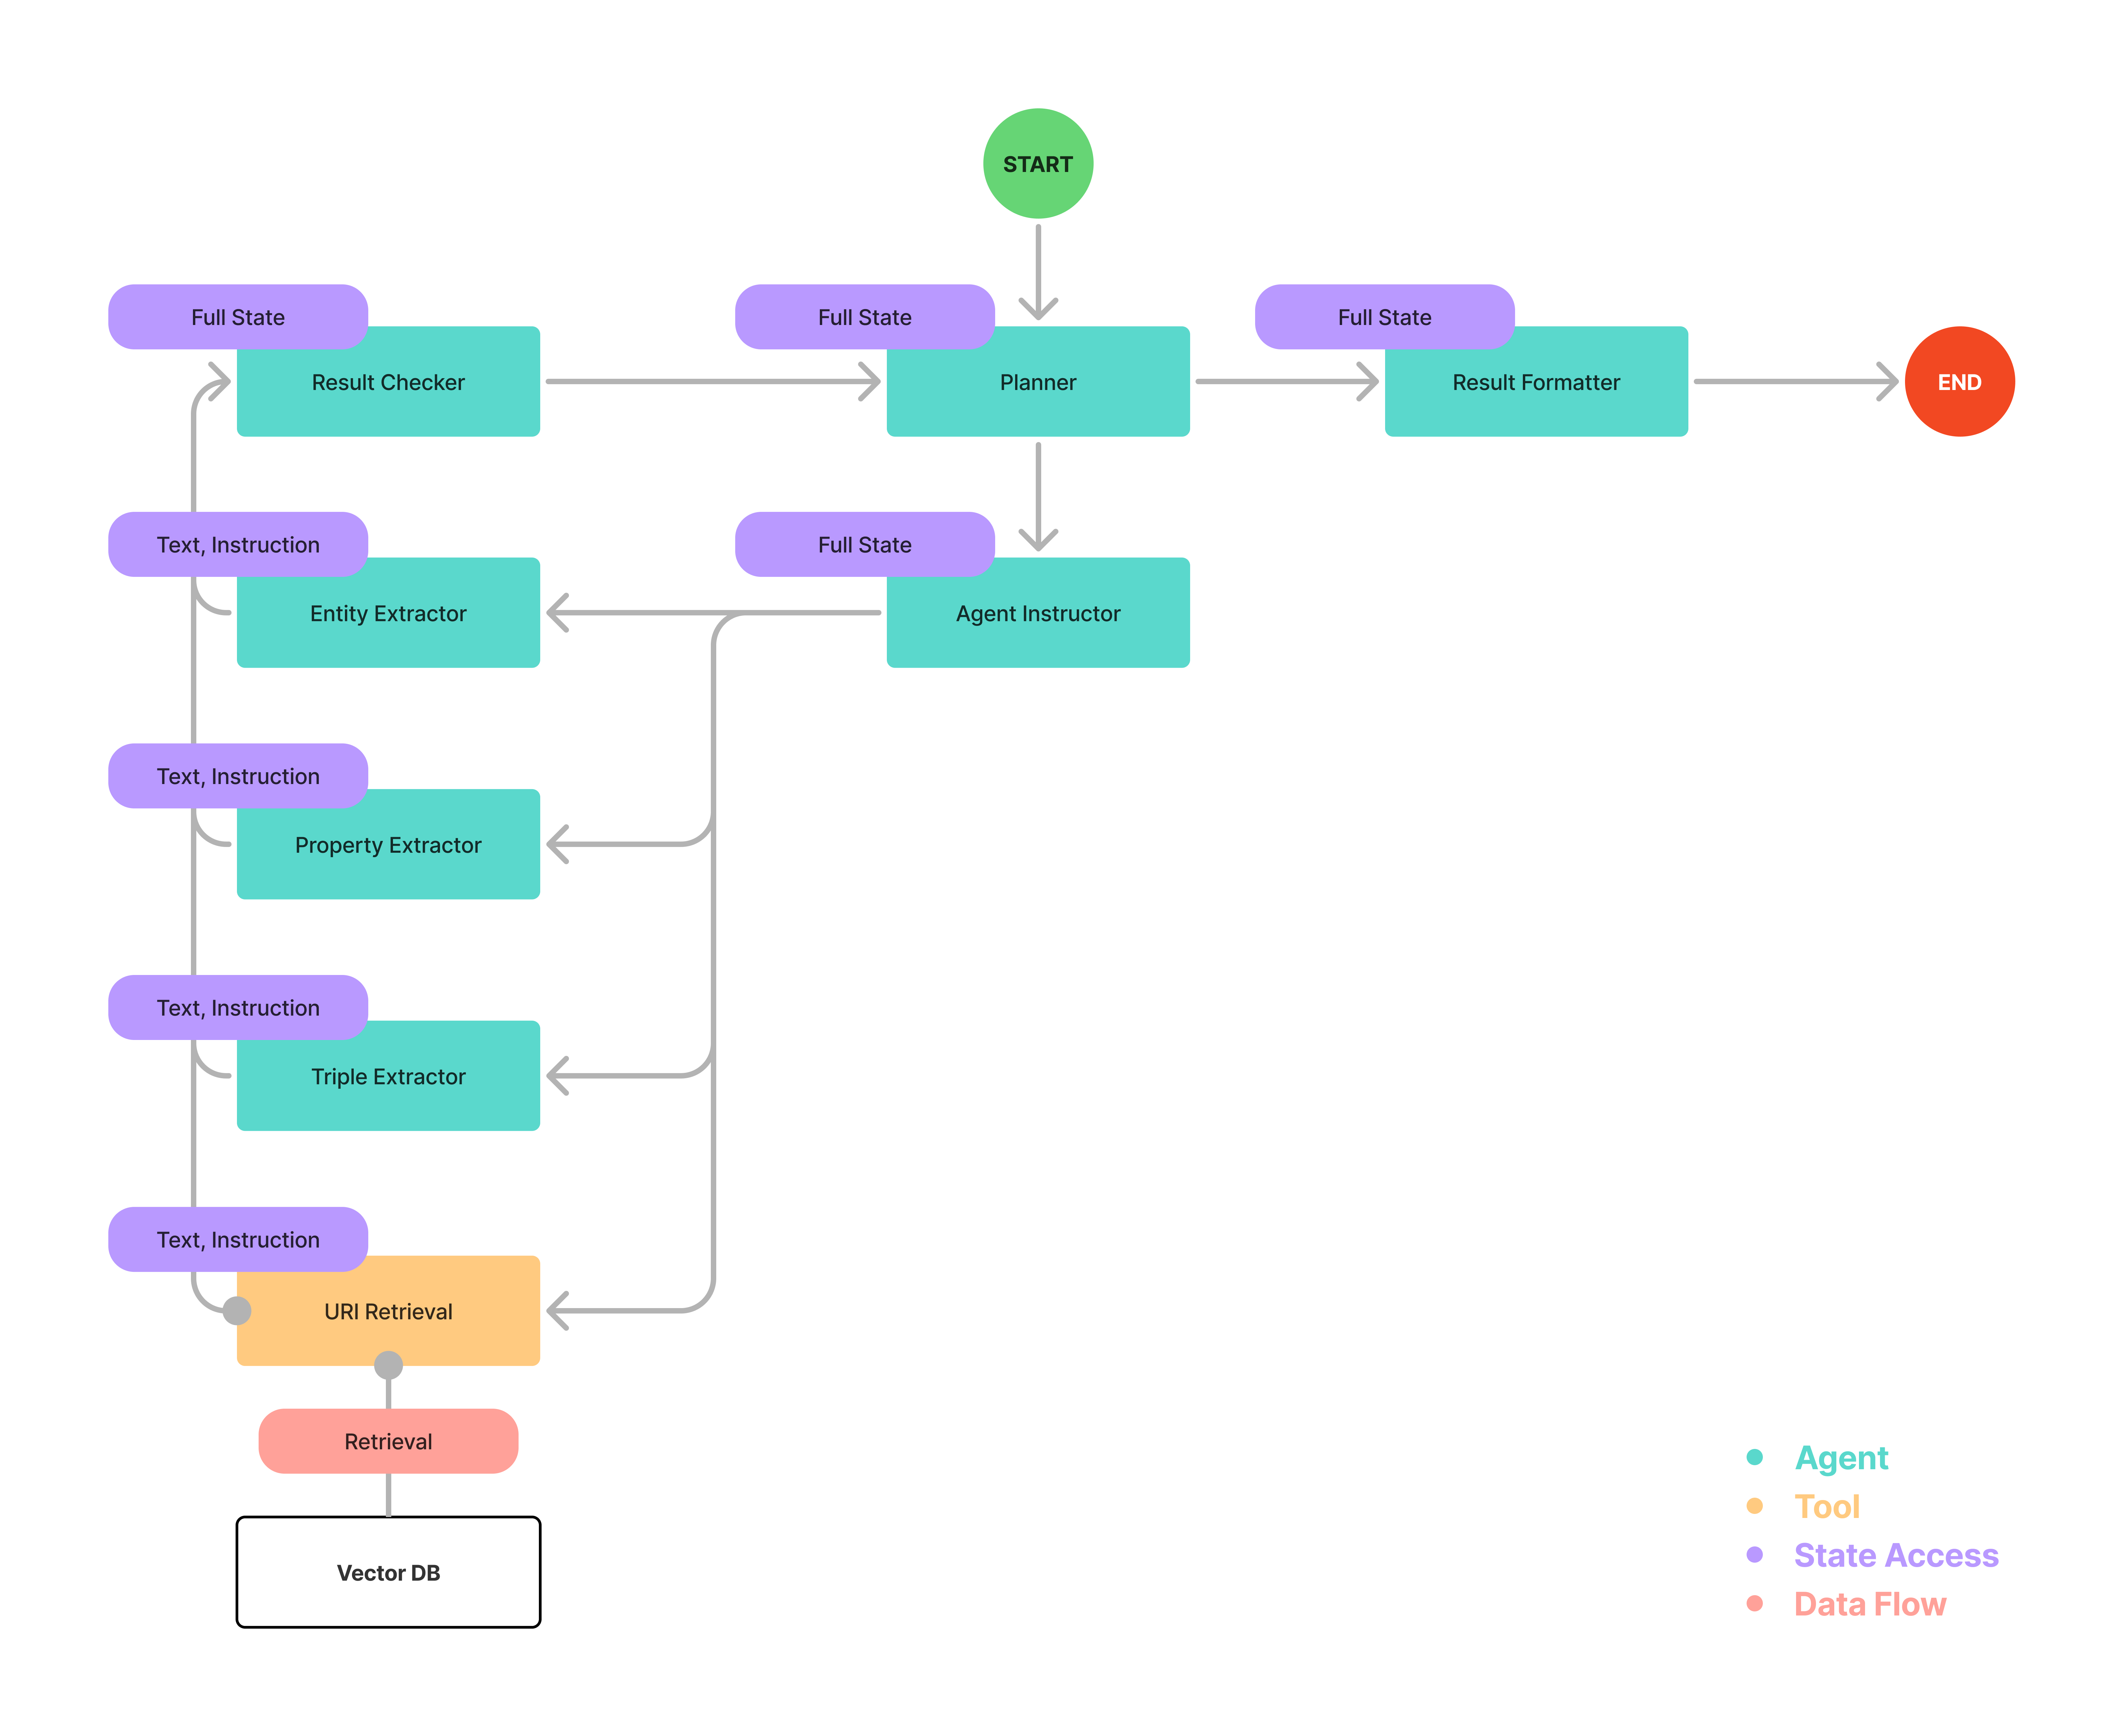
\includegraphics[width=0.7\textwidth]{figures/Splitted Supervisor Architecture.png}
  \caption[Splitted supervisor architecture showing the decomposition of the supervisor agent into specialized sub-agents for better task management]{Splitted supervisor architecture showing the decomposition of the supervisor agent into specialized sub-agents for better task management (self-created)}
  \label{fig:splitted_supervisor_architecture}
\end{figure}

Building on the \textit{baseline architecture}, the \textit{splitted supervisor architecture} (\textit{\ac{SSA}}) extends the supervisor pattern by decomposing the central \textit{supervisor agent} into a series of smaller, specialized agents. In both setups, the main responsibilities remain the same: planning the task, routing it to the appropriate agent or tool with the correct instruction, evaluating the outputs, and either refining the plan or producing a final \texttt{Turtle} string. However, this process proves to be complex, particularly because the idea of using a \ac{MAS} is to enable iterative adjustments to elements such as triples or \ac{URI} mappings.

The \textit{\ac{SSA}} addresses the limitations of \acp{LLM} that struggle with processing many instructions at once or face context window restrictions as prompt sizes grow. To overcome this, the \textit{supervisor agent} role is split into four distinct agents: \textit{planner}, \textit{agent instructor}, \textit{result checker}, and \textit{result formatter}. Additionally, a new \textit{property extractor} for \ac{PropEx} complements the existing specialized agents for \textit{entity extraction} and \textit{triple extraction}. Because the \textit{property extractor} was added later in the iterative process, its evaluation is discussed separately in Section~\ref{subsec:error_message_incorporation}. Figure~\ref{fig:splitted_supervisor_architecture} illustrates the overall structure of this architecture.

To support the expanded supervision logic in the \textit{\ac{SSA}}, the system state was extended to include additional fields beyond \texttt{text} and \texttt{instruction}, while the \texttt{messages} field from the \textit{baseline architecture} was removed. This structured representation separates core \ac{cIE} outputs from orchestration-related data and facilitates reasoning over prior steps. Table~\ref{tab:ssa_state} summarizes the fields used in this architecture.

\begin{table}[h]
  \centering
  \caption{State fields in the \textit{\ac{SSA}} architecture}
  \label{tab:ssa_state}
  \begin{tabular}{p{3cm}p{10cm}}
    \toprule
    \textbf{Name}        & \textbf{Description}                                                                                                 \\
    \midrule
    \texttt{text}        & The document or sentence being processed.                                                                            \\
    \texttt{instruction} & Task-specific instructions for agents or tools.                                                                      \\
    \texttt{call\_trace} & Log of which agent or tool was invoked with which input, used by the \textit{agent instructor} to track system flow. \\
    \texttt{results}     & Collected outputs from specialized agents and the \textit{\ac{URI} retrieval tool}.                                  \\
    \texttt{comments}    & Internal notes written by the \textit{result checker} and \textit{planner agent}.                                    \\
    \bottomrule
  \end{tabular}
\end{table}

At the core of the \textit{\ac{SSA}} is the \textit{planner agent}. It initiates the overall process, develops a step-by-step plan, and decides at each stage whether to proceed or terminate by delegating final output creation to the \textit{result formatter}. If the next action requires agent or tool involvement, the \textit{agent instructor} translates the planner's intention into a concrete call with a matching instruction. This modularity allows each agent to specialize: planning agents can focus on sequencing, while instructors handle syntactic formatting. The \textit{result formatter} follows the same philosophy and is responsible for generating the final output in valid \texttt{Turtle} syntax. In doing so, it combines all partial outputs such as triples and \acp{URI}.

Functioning as the quality control unit, the \textit{result checker agent} plays a critical role in this architecture. This agent evaluates whether the specialized agents are producing meaningful results and identifies missing or incorrect elements. Based on this evaluation, the \textit{result checker agent} provides feedback to the \textit{planner agent} and encourages iterative improvement over the extraction process.

The specialized agents for \textit{entity extraction} and \textit{triple extraction} behave similarly to those in the \textit{baseline architecture}, with adjustments made regarding where their results are stored in the updated state. The new \textit{property extractor} agent was introduced in line with design practices discussed in Section~\ref{sec:agent_design}. Its task is to extract properties from the text, which were previously identified as part of \textit{triple extraction}. The \textit{\ac{URI} retrieval tool} remains conceptually the same as in the \textit{baseline architecture}, though its outputs are now written to the centralized \texttt{results} field.

In summary, the \textit{\ac{SSA}} is an expanded interpretation of the supervisor pattern, aimed at breaking down complex orchestration into smaller, more specialized components. The state has been enhanced to support this increased granularity by providing more transparency and structure, enabling a greater degree of control and adaptability across the agent system.

\subsection{Simplified Splitted Supervisor Architecture}
\label{subsec:simplified_splitted_supervisor}

\begin{figure}[tp]
  \centering
  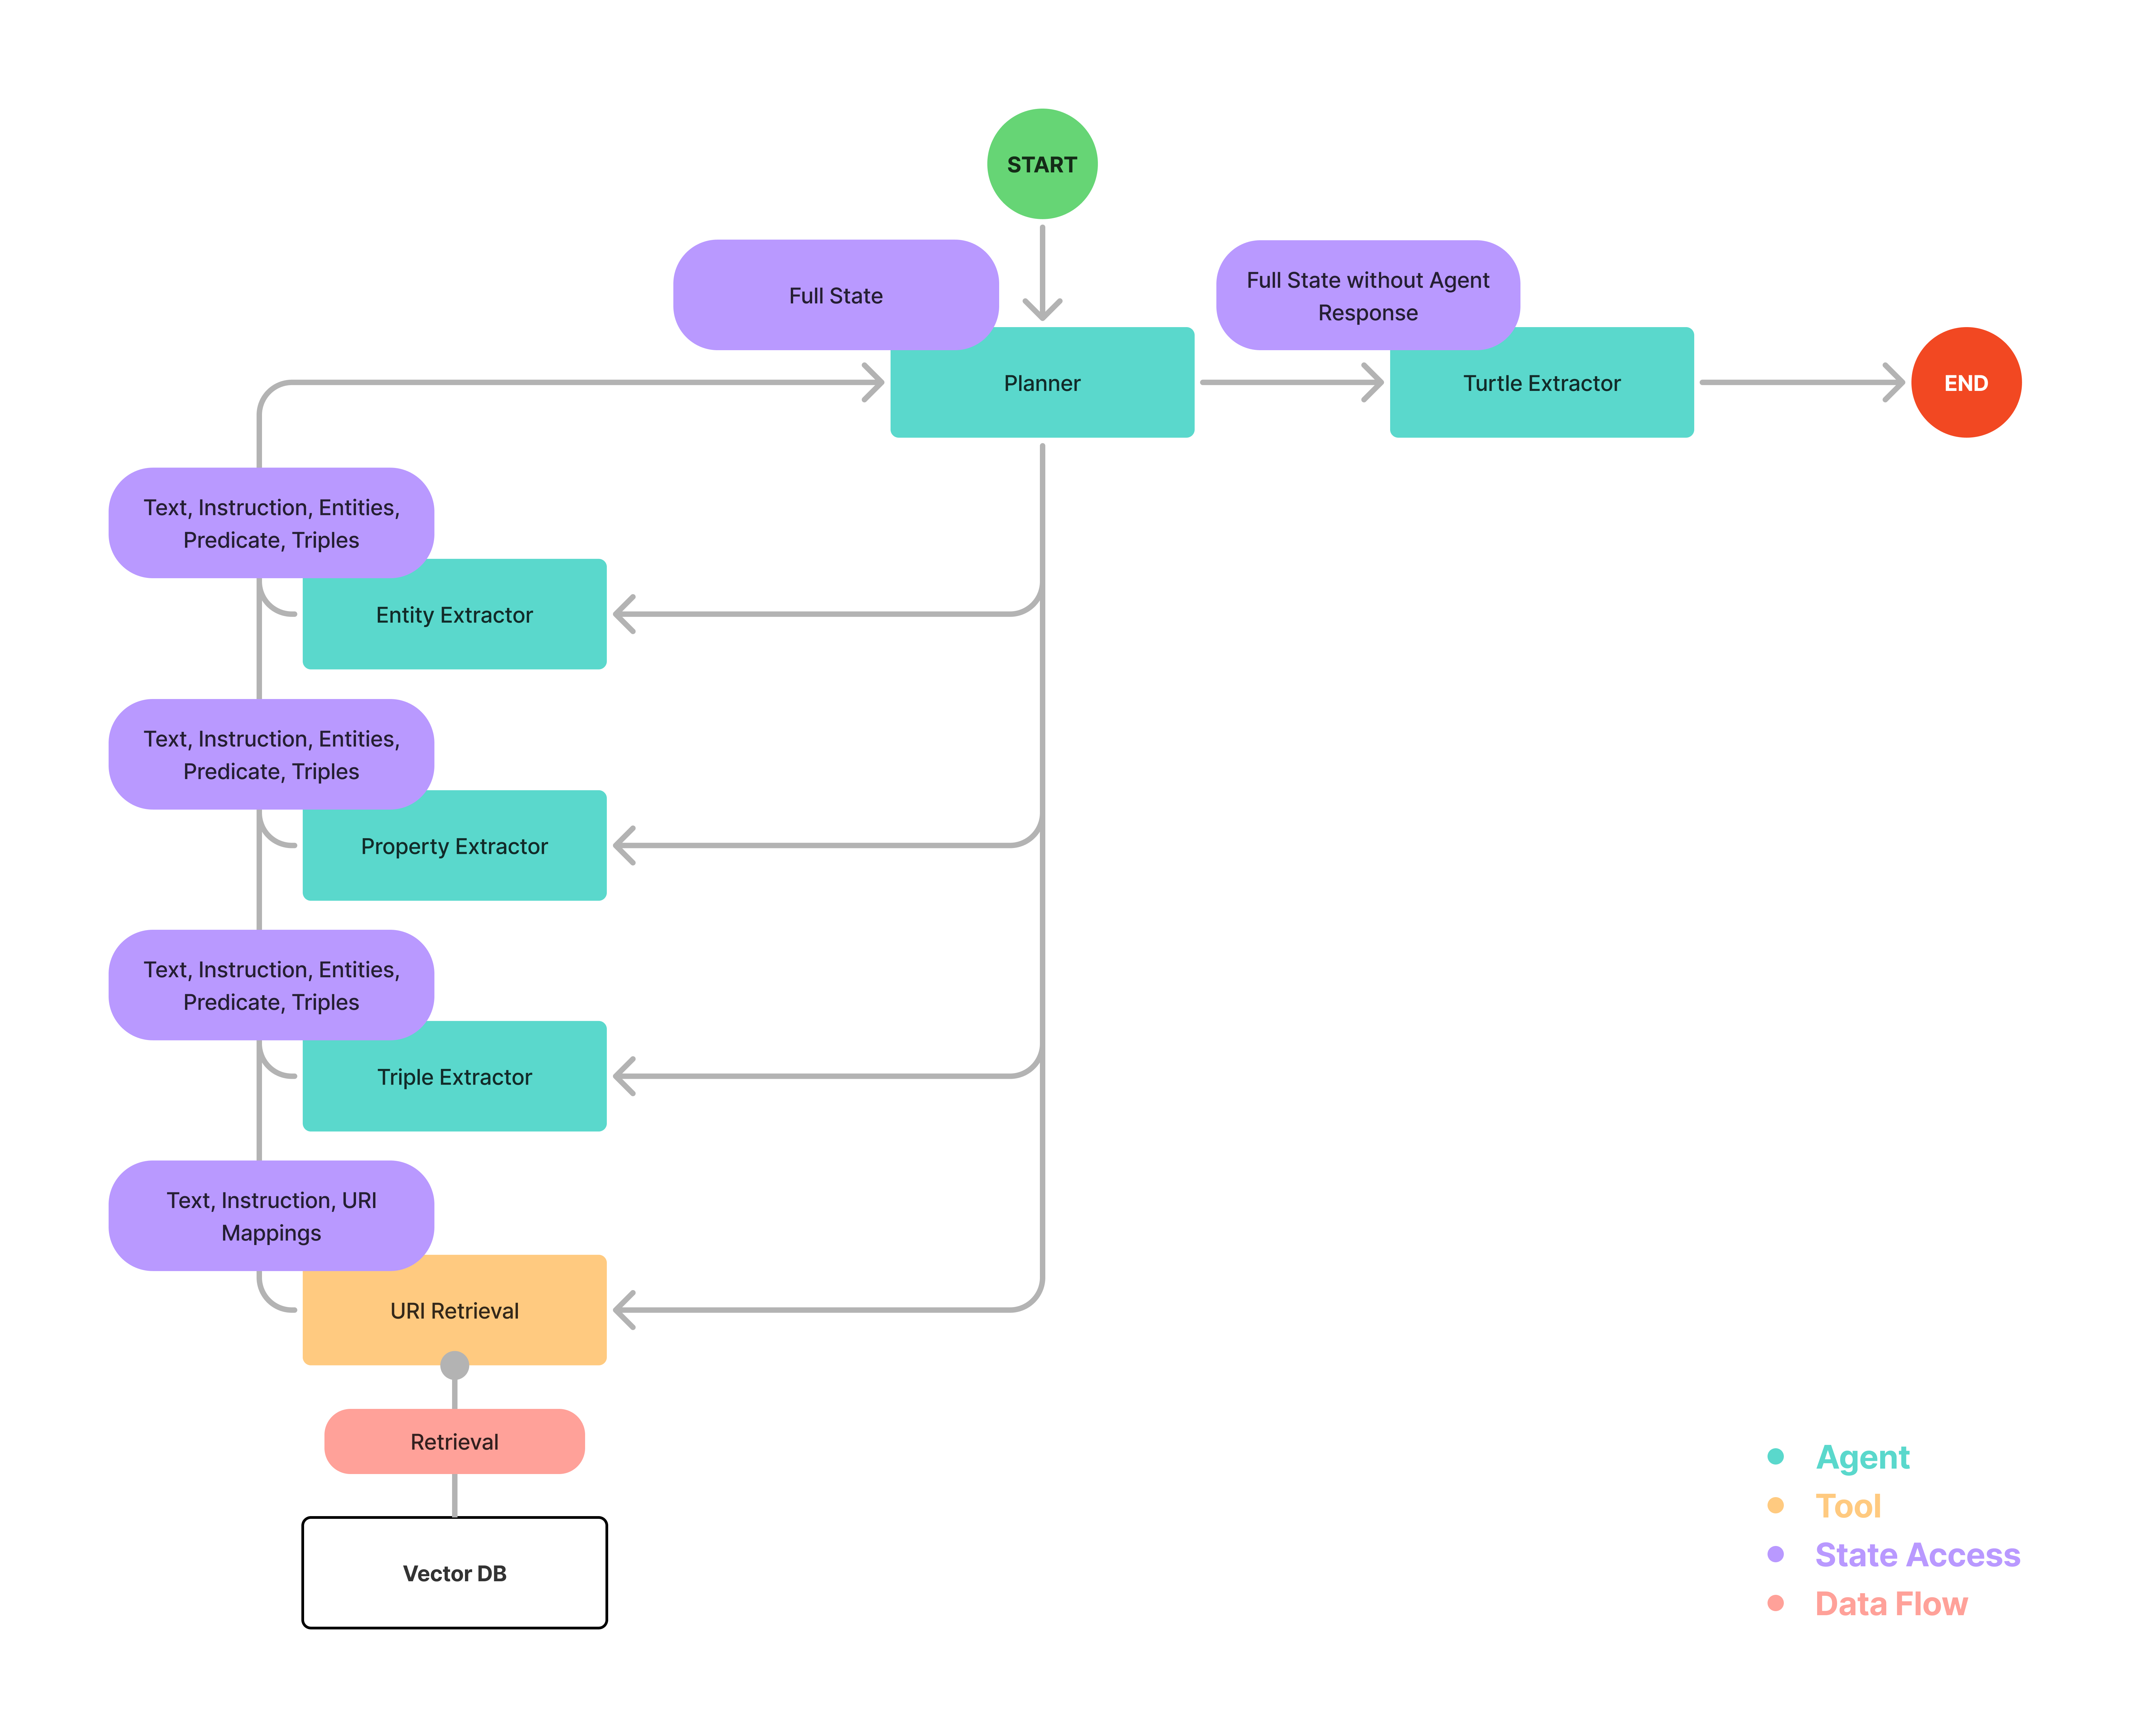
\includegraphics[width=0.7\textwidth]{figures/Simplified Splitted Supervisor Architecture.png}
  \caption[Simplified splitted supervisor architecture showing a streamlined version of the supervisor decomposition with optimized agent interactions]{Simplified splitted supervisor architecture showing a streamlined version of the supervisor decomposition with optimized agent interactions (self-created)}
  \label{fig:simplified_splitted_supervisor_architecture}
\end{figure}

Continuing the principles established in the \textit{splitted supervisor architecture} (\textit{\ac{SSA}}), the \textit{simplified splitted supervisor architecture} (\textit{\ac{SSSA}}) streamlines the agent structure for more efficient interaction and reduced complexity. This design assumes that one agent can still manage all supervision tasks as long as it does not have to generate valid \texttt{Turtle} output or operate over an unstructured state. To accommodate this, the architecture retains all specialized agents from the \textit{\ac{SSA}}, while merging the roles of the \textit{result checker} and \textit{agent instructor} back into the \textit{planner agent}, with output formatting still handled separately. The \textit{planner agent} in this setup functions similarly to the original \textit{supervisor agent} introduced in the \textit{baseline architecture}. A more structured and targeted state is introduced to support these adjustments. Figure~\ref{fig:simplified_splitted_supervisor_architecture} provides an overview of the architecture.

A central change of the \textit{\ac{SSSA}} lies in its redesigned state. The general-purpose \texttt{results} field from the \textit{\ac{SSA}} is replaced by dedicated fields that store the core outputs of specialized agents and tools. This explicit separation improves transparency and enables the \textit{planner agent} to access relevant information directly. Because this streamlined structure removes access to full agent outputs, the state also includes a new \texttt{agent\_response} field. It captures the raw responses from specialized agents and tools, allowing the \textit{planner agent} to verify task completion, detect errors, and initiate corrective actions. Table~\ref{tab:sssa_state} summarizes the fields in this architecture.

\begin{table}[h]
  \centering
  \caption{State fields in the \textit{\ac{SSSA}} architecture}
  \label{tab:sssa_state}
  \begin{tabular}{p{3cm}p{10cm}}
    \toprule
    \textbf{Name}            & \textbf{Description}                                                                                                    \\
    \midrule
    \texttt{entities}        & Output of the \textit{entity extraction} process.                                                                       \\
    \texttt{properties}      & Output of the \textit{property extractor} agent.                                                                        \\
    \texttt{triples}         & Output of the \textit{triple extraction} process.                                                                       \\
    \texttt{uri\_mapping}    & Mapped \acp{URI} from the \textit{\ac{URI} retrieval tool}.                                                             \\
    \texttt{agent\_response} & Raw responses from specialized agents and tools, used by the \textit{planner agent} for quality checks and corrections. \\
    \texttt{messages}        & Dialogue history of the \textit{planner agent} to avoid unintended loops.                                               \\
    \bottomrule
  \end{tabular}
\end{table}

The actual formation of RDF triples remains delegated to the \textit{turtle extractor}, which assembles entities, properties, and \acp{URI} into valid \texttt{Turtle} syntax. This separation of concerns ensures that the planner agent remains focused on flow control and state refinement, rather than performing complex string transformations.

This architectural simplification is motivated primarily by practical considerations. As context window limitations increasingly influence \ac{LLM} performance, minimizing unnecessary content in the state becomes essential. At the same time, the system retains the ability to iterate over the \ac{cIE} process when needed. In doing so, the \textit{\ac{SSSA}} balances agent autonomy with prompt efficiency. It represents a targeted evolution of the supervisor pattern that reduces resource demands while maintaining modular clarity within the \ac{MAS}.

\subsection{ReAct Architecture}
\label{subsec:react}

\begin{figure}[tp]
  \centering
  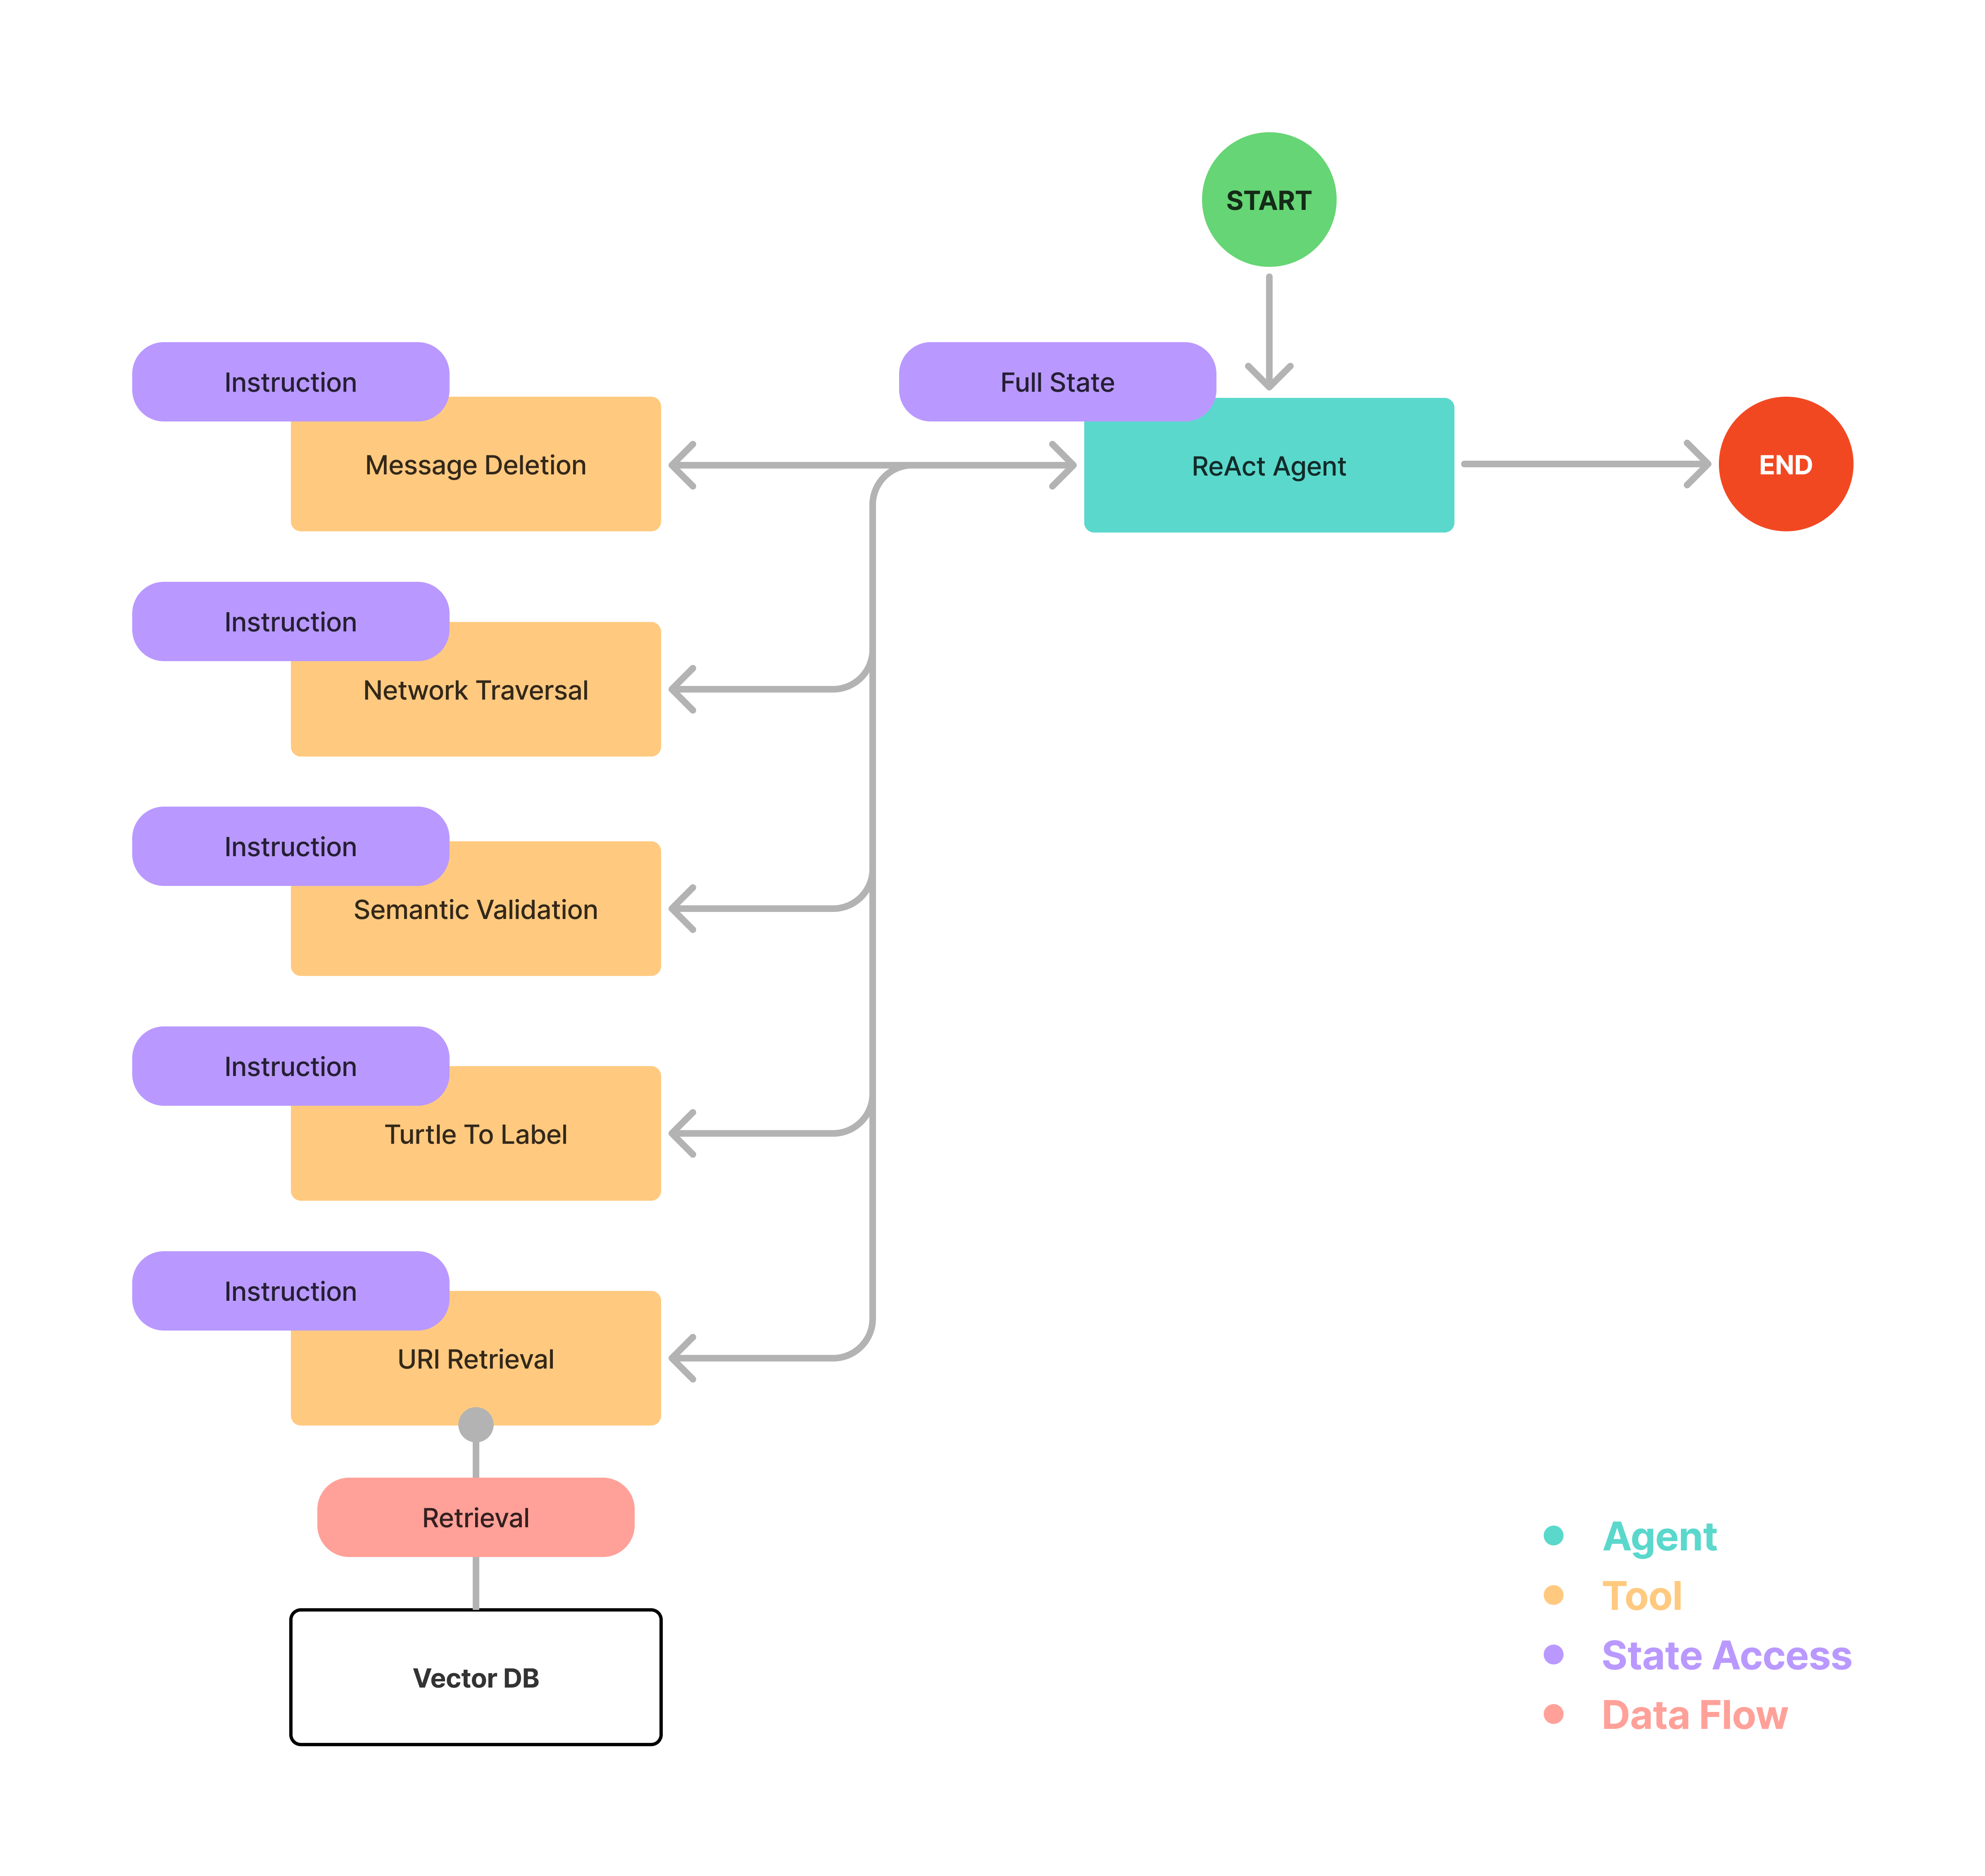
\includegraphics[width=0.6\textwidth]{figures/ReAct Architecture.png}
  \caption[ReAct architecture showing the single-agent approach with reasoning and action capabilities for closed information extraction]{ReAct architecture showing the single-agent approach with reasoning and action capabilities for closed information extraction (self-created)}
  \label{fig:react_architecture}
\end{figure}

Unlike the previously presented solutions, which all rely on a \ac{MAS} to address the complexity of \ac{cIE}, the \textit{ReAct Architecture} takes a contrasting approach. It is designed to evaluate the capabilities of a single agent equipped with reasoning and tool-use abilities \cite{Yao2023}. By eliminating inter-agent communication, the system can focus entirely on tool interactions, reducing coordination overhead and minimizing points of failure.

Another advantage of this joint approach is that it avoids the error propagation that can occur when agents are used to mirror the task-splitting of a traditional \ac{cIE} pipeline. As discussed in Section~\ref{sec:related_approaches}, joint optimization benefits from a single decision point, enabling more coherent outputs. Additionally, reducing the number of agent calls leads to lower inference latency and operational costs.

The state in the \textit{ReAct architecture} is kept intentionally simple. Since only a single agent is involved, the original baseline structure from Section~\ref{subsec:baseline} is reused. Outputs from tools are written to the \texttt{messages} field, allowing the agent to keep track of prior actions and intermediate results.

To support its reasoning capabilities, the agent is equipped with the \textit{\ac{URI} retrieval tool} from the outset. As the architecture proved effective during iterative evaluations, additional tools were developed to extend its capabilities. These include the \textit{network traversal tool}, the \textit{semantic validation tool}, and the \textit{turtle-to-label tool}, each facilitating deeper integration with the underlying knowledge graph. Moreover, a \textit{message deletion tool} was introduced to allow the agent to manage its limited context window by pruning irrelevant or outdated information. The overall tool integration is depicted in Figure~\ref{fig:react_architecture}.

While the \textit{ReAct architecture} does not qualify as a \ac{MAS}, it plays an important role in contrasting complex \ac{MAS} configurations. It represents a simplified single-agent approach that highlights how much can be achieved without multi-agent orchestration. Due to its efficiency and simplicity, it is particularly well-suited for early-stage development and tool testing, making it a logical step within the broader iterative design process. All development steps, including the incremental addition of tools and their evaluated effectiveness, are discussed in detail in Section~\ref{sec:evaluation_configurations}.

\subsection{Network Architecture}
\label{subsec:network}

\begin{figure}[tp]
  \centering
  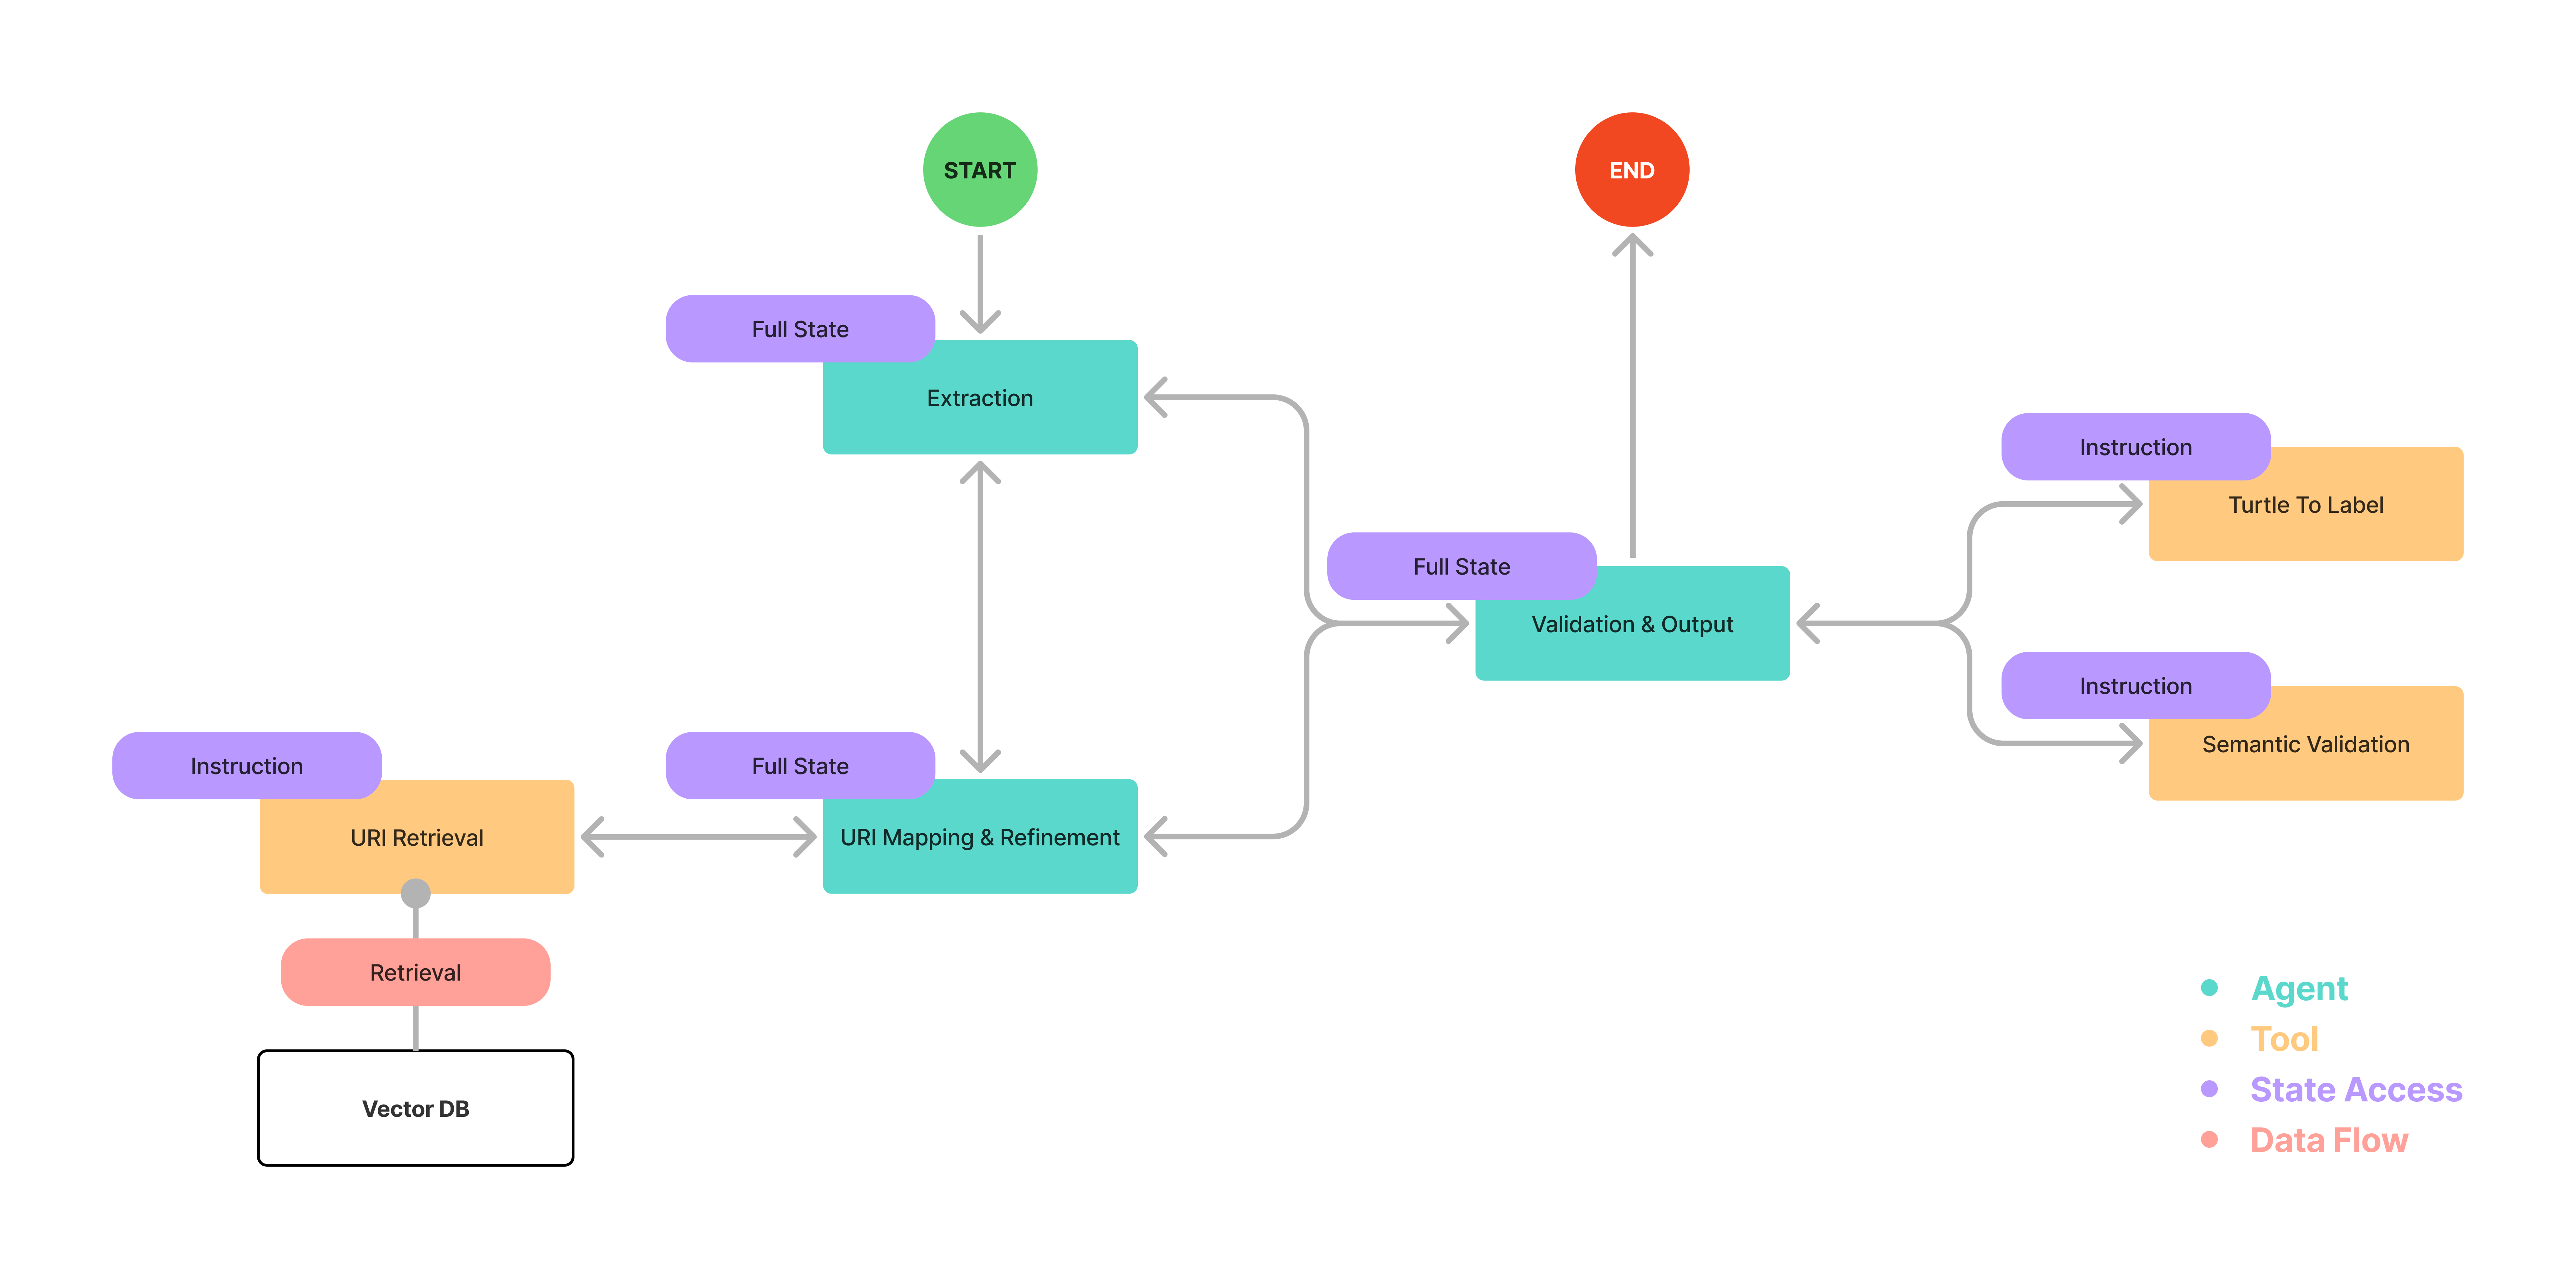
\includegraphics[width=\textwidth]{figures/Network Architecture.png}
  \caption[Network architecture showing the fully connected \ac{MAS} with dynamic routing and reasoning capabilities]{Network architecture showing the fully connected \ac{MAS} with dynamic routing and reasoning capabilities (self-created)}
  \label{fig:network_architecture}
\end{figure}

Building on the network pattern introduced in Section~\ref{sec:multi_agent_systems}, the \textit{Network Architecture} represents a culmination of insights gathered from the design and evaluation of all preceding architectures, tools, and state configurations. It aims to combine the reasoning and validation capabilities developed in the \textit{\ac{SSA}} and \textit{\ac{SSSA}} with the direct triple extraction process featured in the \textit{ReAct Architecture}. Furthermore, this architecture distributes decision-making across all participating agents rather than centralizing it within a single supervisory entity. An overview of the setup is shown in Figure~\ref{fig:network_architecture}.

The underlying state in this architecture extends the structured design of the \textit{\ac{SSSA}} while introducing new elements to better support routing and control logic. It retains \texttt{triples} and \texttt{uri\_mapping}, the latter now enriched with original labels, along with Wikidata-provided labels and descriptions. To facilitate reasoning over prior steps, a \texttt{call\_trace} is reintroduced. Additional fields such as \texttt{last\_call}, \texttt{last\_response}, \texttt{agent\_instruction}, and \texttt{tool\_call} capture the most recent interactions and instructions, enabling efficient forwarding and decision-making. Unlike previous designs, this architecture avoids cumulative state growth, except for the \texttt{call\_trace}, thereby reducing context size and emphasizing concise, high-value information for agent reasoning. The \texttt{messages} field is preserved solely to store the final output string for interoperability with the evaluation framework.

\begin{table}[h!]
  \centering
  \caption{State fields of the network architecture}
  \label{tab:network_state}
  \begin{tabular}{p{0.2\linewidth}p{0.65\linewidth}}
    \toprule
    \textbf{Name}               & \textbf{Description}                                                                 \\
    \midrule
    \texttt{triples}            & Extracted triples from the text.                                                     \\
    \texttt{uri\_mapping}       & \acp{URI} with corresponding original labels, plus Wikidata labels and descriptions. \\
    \texttt{call\_trace}        & Log of all agent and tool calls, including inputs.                                   \\
    \texttt{last\_call}         & Most recent agent or tool invocation.                                                \\
    \texttt{last\_response}     & Result of the most recent call.                                                      \\
    \texttt{agent\_instruction} & Instruction received by the agent, forwarded if needed across tool calls.            \\
    \texttt{tool\_call}         & Input for the most recent tool invocation.                                           \\
    \texttt{messages}           & Final output string for compatibility with the evaluation framework.                 \\
    \bottomrule
  \end{tabular}
\end{table}

From an agent perspective, the architecture employs three distinct agents with full read access to the complete state. In contrast, tools only receive the input specified in the \texttt{tool\_call} field. Granting agents full-state visibility allows them to make more informed decisions about subsequent actions within the overall flow.

The initial entry point for processing is the \textit{Extractor Agent}, which mirrors the core responsibilities of the main agent in the \textit{ReAct Architecture}, while delegating \ac{URI} mapping, validation, and \texttt{Turtle} output to separate components. It is the only agent permitted to write to the \texttt{triples} field.

Handling the \ac{URI} mapping is the responsibility of the \textit{\ac{URI} Mapping and Refinement Agent}. This agent serves as the central unit for generating and updating \ac{URI} mappings and is the only component allowed to write to the \texttt{uri\_mapping} field. It is tightly coupled with the output of the \textit{Extractor Agent} and utilizes the \textit{\ac{URI} Retrieval Tool} to resolve surface forms into structured Wikidata entities and relations.

Validation and output formatting are conducted by the \textit{Validation and Output Agent}. This agent prevents hallucination and ensures semantic correctness by validating triples based on features retrieved from the knowledge graph. To do so, it employs both the \textit{Semantic Validation Tool} and the \textit{Turtle-to-Label Converter}. If any extracted triple fails validation, the agent attempts to refine or regenerate it, either by re-engaging the \textit{Extractor Agent} or by forwarding the task to the \textit{\ac{URI} Mapping and Refinement Agent}, depending on the assumed source of error.

Overall, the network architecture reflects the lessons learned from previous iterations. It omits unpromising tools, makes use of a highly structured and minimal state, and adheres to a fully distributed decision-making strategy. While still grounded in the \ac{MAS} paradigm, it reduces coordination overhead and context consumption to a minimum.

\section{Agent Tools}
\label{sec:agent_tools}

Agents across the different architectures form the backbone of the approach to \ac{cIE}. However, since \acp{LLM} are inherently limited in their up-to-date knowledge and may hallucinate information, as discussed in Section~\ref{sec:language_models}, additional support is required. In this work, such support is provided exclusively through \textit{data tools} (see Section~\ref{sec:agent_tools}), as all tools operate by accessing external data sources. These tools address both reliability concerns and performance limitations, enabling agents to retrieve accurate, contextually relevant information during the extraction process.

Two general categories of tools are introduced in this work. The first category focuses on integrating knowledge graph information. This includes the \textit{uri retrieval tool} (Section~\ref{subsec:uri_retrieval}), the \textit{network traversal tool} (Section~\ref{subsec:network_traversal}), the \textit{semantic validation tool} (Section~\ref{subsec:semantic_validation}), and the \textit{turtle-to-label tool} (Section~\ref{subsec:turtle_to_label}). These tools enable agents to interact with and reason over structured external knowledge.

The second category supports system-level coordination. In this work, only one such tool is introduced: the \textit{message deletion tool} (Section~\ref{subsec:message_deletion}), which is used to manage context size and prevent prompt overflow in long-running agent interactions.

\subsection{\ac{URI} Retrieval}
\label{subsec:uri_retrieval}

The \textit{\ac{URI} retrieval tool} remains a central component in solving the \ac{cIE} task. While various \ac{LLM}-based agents are capable of extracting free-form triples, the core challenge lies in mapping these triples correctly to the underlying knowledge graph. This mapping capability is provided through the \textit{\ac{URI} retrieval tool}, which enables interaction with the knowledge graph.

Its core function is to receive search terms from an agent and perform similarity-based retrieval using sentence embeddings and cosine similarity. Search terms can be iterated and varied by the agent, for example by changing the phrasing, the search mode, or the filter settings. This flexibility allows for multiple retrieval attempts, potentially improving mapping performance.

In order to support this mechanism, the tool maintains three search indices, each generated by embedding specific textual representations from the knowledge graph. These include the \texttt{rdfs:label}, the \texttt{rdfs:description}, and example triples for properties. For the latter, Wikidata provides example triples for many properties, which are reformulated as complete sentences to support semantic encoding of relational context. The construction of these indices is based on Wikidata, the only knowledge graph used throughout this work’s evaluation.

The creation of the search indices follows a structured multi-step pipeline. First, documents are loaded from a selected dataset split, such as the test set of the synthIE dataset. Second, all entities and properties referenced in these documents are extracted by identifying the \acp{URI} of subjects, properties, and objects. For each subject and object, the corresponding \texttt{rdfs:label} and \texttt{rdfs:description} are retrieved from Wikidata. For each property, in addition to the label and description, an example triple that demonstrates the property’s usage is also retrieved.

In the next step, these textual representations are embedded and stored in separate search indices. The \texttt{rdfs:label} values are embedded into a label index, the \texttt{rdfs:description} values into a description index, and the example triples into an example index. Alongside the embeddings, relevant metadata is stored with each entry. This includes the corresponding \ac{URI}, the type of the resource (entity or property), the \texttt{rdfs:label} (for entries in the description and example indices), the \texttt{rdfs:description} (for entries in the label and example indices), and the example triple itself (for properties in both the label and description indices).

To control retrieval behavior, the tool interprets two parameters, \textit{search mode} and \textit{filter mode}. The \textit{search mode} selects the semantic space used for similarity retrieval, that is, whether to search on the labels index, the descriptions index, or the examples index. The \textit{filter mode}, in contrast, restricts retrieval to either entities or properties. This distinction enables more accurate matching and reduces noise, especially when agents provide ambiguous input.

Through the iterations, the tool is tested in multiple configurations, initially without any search mode, then with search modes enabled, followed by a combination of search and filter modes, and finally in a setup that uses only filter modes together with a search mode for example-based search for properties. Details on these configurations are provided in Section~\ref{sec:evaluation_configurations}.

Internally, the \textit{\ac{URI} Retrieval Tool} parses the agent’s instruction, determines the appropriate search and filter modes per term, and executes a cosine similarity search using the term embedding over the selected index. The top result includes the matching entry’s \texttt{rdfs:label}, \texttt{rdfs:description}, and \ac{URI}.

Architectures sensitive to context limitations may encounter issues when the tool returns extensive candidate lists, which is primarily caused by an excessive number of search terms. To address this, the tool supports a compact output mode. In this mode, an additional \ac{LLM} call is used to evaluate whether a specific result matches the query. The response is reduced to a simplified \ac{URI} mapping that includes only the selected \ac{URI} and a brief justification, omitting alternative matches and detailed descriptions. This compact output is used in configurations of the \textit{Baseline Architecture}, the \textit{\ac{SSA}}, and the \textit{\ac{SSSA}}, with the exception of the initial baseline version.

In summary, the \textit{\ac{URI} Retrieval Tool} equips agents with retrieval-augmented access to structured knowledge. By indexing key components of Wikidata and offering fine-grained retrieval controls, it supports precise \ac{URI} mapping in a variety of architectures. Its flexibility and accuracy-critical role led to extensive iterations throughout this work, as discussed in Section~\ref{sec:evaluation_configurations}.

\subsection{Network Traversal}
\label{subsec:network_traversal}

The \textit{network traversal tool} represents a further step in incorporating knowledge graph information into the agent workflow. Its main purpose is to support agents in addressing the challenge of selecting appropriate properties, particularly in cases where the input sentence does not contain the exact label of the target property. This issue could lead to the selection of super-properties or sub-properties. By querying structural information from the knowledge graph, the tool enables agents to explore property hierarchies and make more informed decisions.

To achieve this, the tool executes \ac{SPARQL} queries on Wikidata, focusing on the \textit{subproperty of} relation. These queries retrieve both direct super-properties and sub-properties of a given property. To enhance the output's usability, labels are also queried for each retrieved property. Where available, example triples are included for additional context. The resulting output provides related properties and supporting examples, enabling an agent to assess semantic proximity.

An illustrative example can be found in the property hierarchy involving \texttt{member of political party} (\texttt{P102}). This property is a subproperty of \texttt{member of} (\texttt{P463}), which in turn is a subproperty of \texttt{part of} (\texttt{P361}). Suppose an agent extracts the triple \textit{Angela Merkel; member of; CDU}. The tool could then reveal in the hierarchy both \texttt{part of} with the example \textit{ear; part of; head} and \texttt{member of political party} with the example \textit{Eleanor Roosevelt; member of political party; Democratic Party}. In such a straightforward case, an agent could recognise that \texttt{part of} is too general, while \texttt{member of political party} better captures the intended meaning, since the CDU is a political party.

In some cases, individual properties are connected to a large number of related properties, which may result in long and unordered outputs. As shown by \citet{Hsieh2024}, \acp{LLM} can face difficulties in prioritizing relevant information in long-context scenarios. To mitigate this, additional filtering mechanisms were introduced. Later iterations of the tool included support for inspecting property constraints to assess type compatibility. In Wikidata, these constraints are accessible through qualifiers attached to properties.

In this tool, property constraints are used to assess whether a triple’s subject and object match the expected types. Two constraint types are relevant: the \textit{subject type constraint} defines which class the subject of a property should belong to, and the \textit{value type constraint} specifies the required class for the object. For example, the property \textit{member of political party} (\texttt{P102}) in Wikidata typically has a subject type constraint of \textit{human} (\texttt{Q5}) and a value type constraint of \textit{political party} (\texttt{Q7278}). A triple such as \textit{(Angela Merkel; member of political party; CDU)} therefore satisfies both constraints, since \textit{Angela Merkel} is a human and \textit{CDU} is a political party.

Using this information, the tool extends its \ac{SPARQL} query to determine whether the subject and object types in a candidate triple align with the constraints of a given property. To increase flexibility, the system allows for one level of abstraction by including the direct superclass of each type. This choice is made to avoid the risk of infinite expansion when traversing class hierarchies, which may occur in unbounded queries against Wikidata.

Through the network traversal tool, agents gain access to structural and semantic context that allows them to refine extracted triples. The tool supports identification of overly broad or overly narrow property selections. However, its usage can introduce considerable overhead due to the potentially large number of returned results. Agents must therefore balance constraint alignment with semantic appropriateness, avoiding overfitting to constraints while maintaining accuracy in property selection.

\subsection{Semantic Validation}
\label{subsec:semantic_validation}

Language models are prone to hallucinations and typically lack the built-in capability to verify their own outputs, as discussed in Sections~\ref{sec:language_models} and~\ref{sec:multi_agent_systems}. To address this limitation, the semantic validation tool was introduced. Similar to the approach used in the network traversal tool, it focuses on type restrictions associated with properties in extracted triples. However, it relies on a pre-filtered, loop-free class hierarchy derived from Wikidata\footnote{The underlying datasets for the semantic validation tool are available at: Wikidata class hierarchy \url{https://github.com/maxlautenbach/CIExMAS/blob/main/infrastructure/classes.nt} and Wikidata property hierarchy \url{https://github.com/maxlautenbach/CIExMAS/blob/main/infrastructure/all_properties.ttl}}, which allows efficient validation across the full ontology.

The tool receives a complete \texttt{Turtle} string as input. This string is parsed and split into individual triples, with each triple further decomposed into subject, property, and object. For each property, the tool retrieves any subject and value type constraints defined in Wikidata (see example in Section~\ref{subsec:network_traversal}) and compares them to the actual types of the subject and object. The output indicates whether the triple satisfies these constraints. If a check fails, the tool also returns the expected subject and object types to support corrective action by the agent.

Despite its simplicity, the semantic validation tool provides a valuable mechanism for improving result quality. It helps agents detect cases where a chosen property may be semantically inappropriate, even when descriptions or examples retrieved by the \ac{URI} retrieval tool appear correct. In this way, the tool serves as a knowledge-aware safety net and provides a foundation for iterative improvement.


\subsection{Turtle to Label}
\label{subsec:turtle_to_label}

Throughout development, agents occasionally produced incorrect \acp{URI} due to copy failures or internalized associations from prior knowledge. Given that Wikidata is one of the largest publicly available knowledge graphs, it is likely that parts of it were included in the training data of various \acp{LLM}. As a result, agents may generate \acp{URI} based on memorized content rather than verified information. This introduces a particular risk in CIExMAS, where precise usage of \acp{URI} is essential.

Wikidata follows a consistent structure across entities, properties, and their relationships. At the same time, it distinguishes between the namespace used to define metadata such as labels or descriptions and the one used for actual property assertions. Since other tools in this work, particularly those relying on \ac{SPARQL} queries, depend on correctly defined property \acp{URI}, namespace mismatches can lead to tool failures or incorrect results. This makes it critical to detect and correct such errors before further processing.

To address these issues, the \textit{turtle-to-label tool} processes the final \texttt{Turtle} output and attempts to retrieve the human-readable \texttt{rdfs:label} for each part of every triple. This is done by executing \ac{SPARQL} queries on Wikidata. If a query fails, it typically indicates that the corresponding \ac{URI} is invalid or refers to an incorrect namespace. In addition to flagging invalid \acp{URI}, the tool detects whether a \ac{URI} exists but lacks an English label, and communicates this to the calling agent.

When hallucinated \acp{URI} are generated, the tool highlights these by re-outputting the free-form triples derived from the text, allowing agents to fall back on reasoning over textual content. In doing so, the tool helps expose incorrect or unresolvable references and supports downstream correction.

Overall, the \textit{turtle-to-label tool} offers a lightweight mechanism for integrating with the knowledge graph and validating agent outputs. Used in tandem with the \textit{semantic validation tool}, it can strengthen the agent’s ability to detect errors and improves the final quality of extracted triples.

\subsection{Message Deletion}
\label{subsec:message_deletion}

Context bloating has been addressed repeatedly across chapters, particularly through the careful design of agents, states, and tools. An additional strategy introduced in this work is to provide agents with the ability to manage the context proactively. To support this, the \textit{message deletion tool} was implemented.

This tool allows agents to delete individual messages from the state using an internally assigned identifier. Its development was motivated especially by the needs of the \textit{ReAct architecture}, where a single \texttt{messages} field stores all outputs from the main agent and tools. Since components such as the \textit{network traversal tool} or the \textit{\ac{URI} retrieval tool} often produce verbose outputs, this field can quickly become a bottleneck in terms of context size. At the same time, agents are capable of reusing or summarising content. Consequently, the tool enables them to remove outdated or redundant messages and optionally replace them with more concise summaries of the knowledge extracted.

When used in CIExMAS, the \textit{message deletion tool} was implemented exclusively in the \textit{ReAct architecture} and limited to removing entries from the \texttt{messages} field. Its primary purpose was to enable targeted pruning of verbose tool or agent outputs in order to manage context size. The practical implications of using this tool in the \textit{ReAct architecture} are discussed in Section~\ref{subsec:one_agent_architecture_tool_usage}.

\section{Iterative Prompt Engineering}
\label{sec:iterative_prompt_engineering}

As outlined in Sections~\ref{sec:ai_agents} and~\ref{sec:multi_agent_systems}, \acp{LLM} are highly sensitive to prompt design. Finding suitable prompts is therefore a non-trivial and often challenging task. Since this work focuses primarily on developing a range of multi-agent architectures and demonstrating that knowledge graph incorporation improves performance, the prompt engineering process was conducted manually and iteratively.

The general strategy follows the principles discussed in Section~\ref{sec:agent_design}. Prompts were written and refined to be solvable by a human, aiming to leverage the reasoning capabilities of \acp{LLM} without exceeding their limitations. In addition, most prompts include examples to support \ac{ICL}. Depending on the use case, these examples either illustrate tool instructions or are drawn directly from the dataset used in a specific task, such as entity extraction. In the latter case, original text passages were combined with the expected entities to show the agent which types of triples are considered relevant.

Another technique applied throughout this process is guided \ac{CoT}. Agents were explicitly instructed to follow a predefined and prompted chain of thought. Most prompts consist of a consistent structure, including a role introduction, a description of available tools, if applicable, a list of guidelines, illustrative examples, and finally the input state. The guidelines serve to handle edge cases and known failure modes, whereas the role introduction typically remains unchanged across different prompt iterations.

As discussed in Section~\ref{sec:agent_design}, clear tool descriptions are essential to enable proper tool usage. In CIExMAS, tools are embedded directly in the prompt. Each is presented with an identifier, a name, and a descriptive text. This description also defines the expected instruction format. This is particularly relevant for tools such as the \textit{\ac{URI} retrieval tool}, where specific search and filter modes must be communicated to the agent through the prompt.

In summary, prompt engineering in CIExMAS is realized as a manual, iterative process. The design principles are aligned with best practices observed in prior research, emphasizing human readability, structured layout, and the inclusion of well-selected examples, either for tool usage or for solving the core extraction tasks. The individual prompts used in this work can be found in the snapshots of the configurations described in Section~\ref{sec:evaluation_configurations}.

\section{Error Handling}
\label{sec:error_incorportion}

As \acp{LLM} are designed to generate unstructured text, problems can arise when a specific output format or the use of predefined tags is expected. One solution lies in leveraging the reasoning and looping capabilities of agent systems to incorporate error messages into the agentic flow. This allows agents to detect and potentially correct faulty behavior, particularly when error messages are well-defined and understandable.

As described in Chapter~\ref{ch:approach}, the consistent parsing strategy across CIExMAS is the use of XML tags to mark key elements in agent responses, such as the identifier of the next agent or the corresponding instruction. Therefore, each agent is prompted to return information in an XML-tagged format, which is subsequently parsed during execution. For example, the agent output is scanned for a \texttt{<goto>} tag to determine which agent or tool should be called next. Similarly, the \texttt{<instruction>} tag is used to extract task-specific input. These parsing routines are vulnerable to failures if tags are missing, malformed, or empty.

To manage such failures, all parsing steps in the agent execution loop are enclosed in \texttt{try}-\texttt{except} blocks. If an expected tag is not found or cannot be interpreted correctly, the system generates a specific error message describing the missing or malformed element. This error is then returned to the calling agent, allowing it to revise its output in the next reasoning step.

Similar mechanisms are implemented for tool inputs. If an agent provides a malformed instruction, such as an undefined search mode for the \ac{URI} retrieval tool, the tool parser triggers an exception and returns a descriptive error message back to the agent. This enables iterative corrections without terminating the execution.

Another source of errors involves incorrect or hallucinated agent outputs. As discussed in Sections~\ref{subsec:semantic_validation} and~\ref{subsec:turtle_to_label}, dedicated tools are used to validate the semantic and syntactic correctness of extracted triples and \acp{URI}. In the final execution step, all generated \texttt{Turtle} outputs are parsed using a \texttt{Turtle} parser to verify compliance with syntax rules. Errors at this stage include undefined prefixes, incorrect namespaces, or invalid characters. These issues are again transformed into structured error messages that can be interpreted by the system and used for further iteration, allowing the system to react appropriately when an error occurs.

Through this layered error handling, CIExMAS can detect and respond to a broad range of issues, from missing XML tags to malformed \texttt{Turtle} syntax. Error messages are returned in a machine-readable format and reintegrated into the agent flow, enabling agents to revise and repeat failed steps. External issues such as context overflows or GPU memory errors remain outside the scope of this system level handling. Nevertheless, within the agentic loop, this approach increases robustness and helps ensure that a valid output can be generated for each datapoint.

\chapter{Evaluation}
\label{ch:evaluation}

This chapter presents the evaluation of the effectiveness of various \acp{MAS} in solving the \ac{cIE} task within the CIExMAS approach. All architectures and configurations were implemented in Python and evaluated within a standardized setup. Section~\ref{sec:evaluation_setup} outlines the core components of this setup, including the datasets, the integration of Wikidata, the language models used, and the employed frameworks. Section~\ref{sec:evaluation_metrics} explains the evaluation metrics that serve as the foundation for comparing different configurations.

The presentation of the results are spread across two sections. Section~\ref{sec:evaluation_overview} presents a benchmark comparison of the best-performing CIExMAS configuration against existing approaches such as the synthIE model~\cite{Josifoski2023} and GenIE~\cite{Josifoski2021}, evaluated on a subset of the test split of the \texttt{synthIE-text} dataset~\cite{Josifoski2023}. Section~\ref{sec:evaluation_configurations}, in contrast, dives into the different CIExMAS configurations and highlights how individual architectural and tool-based iterations influenced performance. Finally, Section~\ref{sec:discussion} synthesizes the results and provides an interpretation in the context of multi-agent design and knowledge graph incorporation.

\section{Evaluation Setup}
\label{sec:evaluation_setup}

This section outlines the experimental setup used to evaluate the effectiveness of the proposed \ac{MAS} architectures for \ac{cIE}. The structure comprises four main components.

First, Section~\ref{subsec:dataset} introduces the datasets and comparison models used in the evaluation. It outlines which splits were selected and provides relevant context for how the evaluation is structured. Second, the process of accessing and interacting with the knowledge graph is described in Section~\ref{subsec:knowledge_graph_access}. This includes technical details regarding how Wikidata was queried or indexed to enable efficient retrieval of relevant information during agent execution.

Section~\ref{subsec:eval_language_models} then presents the language models and providers employed throughout the experiments. These models form the foundation for agent behavior and reasoning across the evaluated architectures. Finally, Section~\ref{subsec:agentic_framework} details the agent framework used to orchestrate interactions between agents and tools. This includes how prompts are assembled, how state transitions are handled, and how tools are invoked. Large parts of the execution and traceability of CIExMAS were monitored using the open-source platform \textit{LangFuse}\footnote{Available at \url{https://langfuse.com}}, which was integrated to support reproducibility and debugging.

\subsection{Dataset and Comparison Models}
\label{subsec:dataset}

The evaluation is based on the synthIE dataset, with one experiment conducted using the REBEL dataset. Both datasets, which are described in Section~\ref{sec:related_datasets}, contain triples that are extracted from a given text. Each extracted triple contains unique identifiers from Wikidata for each part of the triple, which makes them ideal for \ac{cIE}. Each identifier can be resolved within the entity namespace \texttt{https://www.wikidata.org/entity/}.

Both datasets follow a similar structure. They are stored in JSON Lines format, which is a line-separated format consisting of objects that represent entities, relations, and triples. Each line in the file corresponds to one sample, which is a single document with its associated triples.

Each entity and relation, which can also be referred to as a property, is further decomposed into a \texttt{surfaceform} and a \texttt{uri}. The \texttt{surfaceform} corresponds to the textual appearance of the entity or relation in the input text, while the \texttt{uri} denotes the local part of the Wikidata Qname. A Qname itself consists of a prefix (i.e., the namespace) and a local identifier \cite{ASF2010}. For example, the entity \enquote{Angela Merkel} is represented as \texttt{Q567} and can be resolved under the namespace \texttt{https://www.wikidata.org/entity/}. Each triple is composed of subject, property, and object, each following the same structure.

As outlined in Section~\ref{sec:related_datasets}, two variants of the synthIE dataset exist: \texttt{synthIE-code} and \texttt{synthIE-text}. These versions differ in the \texttt{GPT-3.5} model used for text generation. Since the \texttt{synthIE-text} version demonstrated higher performance, it is exclusively used for the final evaluation in this work.

However, all evaluation configurations prior to Section~\ref{subsec:network_traversal} were developed using the \texttt{synthIE-code} variant. The larger amount of available data in this variant allowed for a more extensive development set, increasing the likelihood of identifying edge cases. Specifically, the training split of \texttt{synthIE-code} was used and sorted so that Document ID~1 appears first in the JSON Lines file.

Due to limitations in data quality and the practicality of developing on small example sets, the later stages of development were shifted to the validation split of \texttt{synthIE-text}. This split, which is also sorted by ID, contains the same underlying triples but with different textual phrasing. Since \texttt{synthIE-text} does not provide a training split (see Section~\ref{sec:related_datasets}), the validation set served as a basis for prompt iteration. Its higher text quality also facilitates the resolution of edge cases that may be difficult to detect in more ambiguous examples. Furthermore, \texttt{synthIE-text} was eventually no longer used because its size advantage could not be leveraged effectively in the development of CIExMAS.

The final evaluation, applied to CIExMAS configurations and the comparison models, was conducted on the first 50 samples of the sorted test split of \texttt{synthIE-text}. This number was chosen due to limitations in computational resources, particularly relevant for architectures with frequent agent calls, such as the \textit{\ac{SSA}} or \textit{\ac{SSSA}}. The use of \texttt{synthIE-text} is further justified by the findings of \citet{Josifoski2023}, who observed improved performance compared to \texttt{synthIE-code} without changes to the underlying triple set. Empirical testing during this work also confirmed a clearer alignment between text and triple content.

To illustrate the distinction between \texttt{synthIE-code} and \texttt{synthIE-text}, the first document from both datasets is shown in the following example. In the \texttt{synthIE-code} version, the sentence reads: \emph{\enquote{'Groovin' Blue' is an album by Curtis Amy, released on Pacific Jazz Records.}} In contrast, the \texttt{synthIE-text} version states: \emph{\enquote{Groovin' Blue was released on Pacific Jazz Records and performed by Curtis Amy.}} While both versions encode the same structured triplets, shown in Table~\ref{tab:triple-example}, the surface form differs. The \texttt{synthIE-text} version more clearly hints at the intended predicate \emph{performer} through the explicit phrase \enquote{performed by Curtis Amy}, whereas in \texttt{synthIE-code} this predicate must be inferred indirectly from the album–artist relationship.

\begin{table}[h]
  \centering
  \begin{tabular}{l l l}
    \toprule
    \textbf{Subject} & \textbf{Property} & \textbf{Object}        \\
    \midrule
    Groovin\_Blue    & record label      & Pacific\_Jazz\_Records \\
    Groovin\_Blue    & performer         & Curtis\_Amy            \\
    \bottomrule
  \end{tabular}
  \caption{Surfaceform Triplets – DocID: 0 – \texttt{synthIE-code} \& \texttt{synthIE-text}}
  \label{tab:triple-example}
\end{table}

To benchmark the performance on the REBEL dataset as well, the first 50 samples from the sorted test split were evaluated. Since CIExMAS was primarily developed using the synthIE dataset, its generalization to REBEL was limited. In testing, none of the CIExMAS configurations achieved an F1 score above 0.1, which led to the exclusion of REBEL from further evaluation. The full test results are documented in Appendix~\ref{sec:rebel_testing}.

The synthIE dataset was ultimately used to evaluate both CIExMAS configurations and the comparison models. For the synthIE model and GenIE (see Section~\ref{sec:related_approaches}), the pre-trained versions provided by \citet{Josifoski2023}\footnote{Available at \url{https://github.com/epfl-dlab/SynthIE}} were used. Although GenIE was originally introduced by \citet{Josifoski2021}, the versions applied here are those retrained and published by \citet{Josifoski2023}. All models are based on the \texttt{Flan-T5} language model, following the setup by \citet{Josifoski2023}, although the original GenIE implementation in \citet{Josifoski2021} was based on \texttt{BART}.

The compared models include \textit{synthIE\textsubscript{T5-base}}, \textit{synthIE\textsubscript{T5-base-SC}}, and \textit{synthIE\textsubscript{T5-large}}, as well as \textit{GenIE\textsubscript{T5-base}} and \textit{GenIE\textsubscript{T5-base-SC}}. The abbreviation \texttt{SC} refers to the subject-collapsed variant, in which all triples sharing the same subject are grouped. These models were chosen because, to the best of current knowledge, they are the only publicly available approaches evaluated on a synthIE dataset and can be readily applied without extensive reimplementation. All comparison models were evaluated on the same subset of 50 documents from the test split of \texttt{synthIE-text}, a limitation imposed by the available hardware resources.

In summary, the sorted 50-sample test split of the \texttt{synthIE-text} dataset serves as the primary benchmark for both CIExMAS and the comparison models. This setup enables the evaluation of different configurations and allows a direct comparison of their respective performance levels.

\subsection{Knowledge Graph Access}
\label{subsec:knowledge_graph_access}

As outlined in multiple sections concerning knowledge graph incorporation tools (cf. Section~\ref{sec:agent_tools}), it is necessary to provide the agent system with direct access to Wikidata as the underlying knowledge graph. To achieve lower latency, this is realized through a setup consisting of Qdrant as a vector database, Redis as a key-value store, and Apache Jena Fuseki as a local \ac{SPARQL} endpoint. All components are hosted on a virtual private server, which, in practice, showed reduced latency compared to direct usage of Wikidata’s public \ac{SPARQL} endpoint. Nonetheless, direct access to the public \ac{SPARQL} endpoint is required in the \textit{network traversal tool} and the \textit{turtle-to-label tool} to retrieve specific restrictions.

The \textit{\ac{URI} retrieval tool} (cf. Section~\ref{subsec:uri_retrieval}) requires a search index to generate relevant mappings. A database supporting similarity search was therefore necessary to enable the described approach, a requirement fulfilled in this setup by Qdrant. In the present evaluation, each search index corresponds to one collection within the hosted Qdrant vector storage.

To populate the Qdrant collections, relevant entity and property data were pre-collected from all datasets used during development and benchmarking. Specifically, the first 50 samples from the sorted validation and test splits of the \texttt{synthIE-text} dataset, the sorted train and test splits of the \texttt{synthIE-code} dataset, and the sorted test split of the REBEL dataset (cf. Section~\ref{subsec:dataset}) were processed. From these samples, all referenced entities and properties were extracted and indexed into the Wikidata-based collections.

This approach ensures that the agent system can resolve all required \acp{URI} regardless of which dataset is currently used, while also preparing CIExMAS for practical deployment scenarios where operation over the entire knowledge graph is required. It further allows efficient switching between datasets in development and benchmarking without the need to rebuild or reindex the knowledge base.

As previously stated in Section~\ref{subsec:semantic_validation}, semantic validation requires a loop-free hierarchy graph of Wikidata’s entities and properties. In this context, a loop-free hierarchy graph refers to a directed acyclic graph structure derived from the subclass and subproperty relations of Wikidata, where cycles have been removed to ensure consistency during hierarchical reasoning. To make these graphs accessible across multiple machines, an instance of Apache Jena Fuseki was hosted containing a class and a property hierarchy. Due to the reduced size of these graphs, this approach also improved performance compared to direct queries to the Wikidata \ac{SPARQL} endpoint.

The Redis key-value store is employed to accelerate data processing pipelines and debugging. Specifically, Redis stores which data from Wikidata have already been inserted into the Qdrant database. Additionally, it caches labels, descriptions, and types of elements from Wikidata, enabling faster label display. This becomes particularly relevant when benchmarking results are inspected in detail and each \ac{URI} must be transformed into a human-readable label.

In summary, the use of a vector store is essential for addressing the \ac{cIE} task within the CIExMAS framework. Moreover, components such as the triple store and key-value store facilitate distributed access to information and contribute to reduced latency. Together, they ensure that the overhead for preparing and executing the agent system remains low.

\subsection{Language Models}
\label{subsec:eval_language_models}

The choice of a language model is a complex task in the context of a \ac{MAS}. For such a task, the \ac{LLM} must be able to follow prompts, plan, reason about tasks, extract triples, and understand how knowledge graph triples are typically constructed. Furthermore, from the start of the CIExMAS project until its conclusion, multiple models were released. These models had not previously been tested on approaches related to CIExMAS, which meant that the evaluation began from a foundational level.

An additional limitation concerned the benchmarking system and the providers used for development. All benchmarks were executed on two Nvidia A100 GPUs with 48~GB VRAM each. The \ac{LLM} ran using \textit{vLLM}\footnote{Available under \url{https://docs.vllm.ai/en/latest/}}, while the embedding model ran using \textit{Ollama}\footnote{Available under \url{https://ollama.com}}. This setup imposed a practical parameter limit of approximately 120~billion parameters for a 4-bit quantised \ac{LLM}, based on empirical observation, though the exact limit varies between models. Development and evaluation focused on open-source models to ensure traceability in CIExMAS and provide greater flexibility in model use, particularly with regard to fine-tuning or adapting specific model components. This also enabled running evaluations on local servers rather than consuming credits at AI vendors for token-intensive benchmarking.

During the course of the work, \texttt{Llama-3.3-70B} consistently demonstrated the strongest performance in the required capabilities, particularly in executing a \ac{MAS} and following instructions. For this reason, all CIExMAS benchmarks, with the exception of the model variation tests, were conducted using a 4-bit AWQ version of \texttt{Llama-3.3-70B}, namely \texttt{kosbu/Llama-3.3-70B-Instruct-AWQ}\footnote{Available under \url{https://huggingface.co/kosbu/Llama-3.3-70B-Instruct-AWQ}}. The development process was conducted on unquantised versions of the models using the providers \textit{SambaNova Cloud}\footnote{\url{https://sambanova.ai}} and \textit{Cerebras}\footnote{\url{https://cerebras.net}}, which offered significantly faster inference. However, both providers imposed a context length limit of 8192 tokens during the course of the work, which is why a maximum context of 8192 tokens was used throughout this thesis.

The achieved performance of \texttt{Llama-3.3-70B} was in line with the benchmarks results reported by \citet{Meta2024}, which demonstrated results comparable to \texttt{GPT-4o} and \texttt{Claude-3.5-Sonnet}. These models were considered state-of-the-art at the time but required more parameters and were not open source. The \texttt{Llama-3} series follows a similar architecture to \texttt{GPT} models, yet benefits from training on a large volume of high-quality data. This approach allowed the parameter count to be reduced to 405~billion for \texttt{Llama-3} and 70~billion for \texttt{Llama-3.3} while maintaining competitive performance~\cite{Grattafiori2024,Meta2024}.

More recently, Google released \texttt{Gemma-3}, an open-source model ranked among the best in the human-evaluated LMSys Chatbot Arena~\cite{Chiang2024}, while maintaining a comparatively low 27~billion parameters~\cite{Team2025}. In publicly available benchmarks such as \textit{MMLU-Pro} (see Section~\ref{sec:language_models}), \texttt{Gemma-3} scored slightly lower than \texttt{Llama-3.3-70B}. In CIExMAS experiments, it additionally exhibited weaknesses in instruction following and logical agent flow execution.

Newer model architectures, such as \textit{Mixture-of-Experts} and reasoning models, notably emerged with the release of \texttt{DeepSeek-R1}, \texttt{Kimi-K2} and \texttt{Llama-4}~\cite{KimiTeam2025,DeepSeekAI2025,MetaAI2025}. These models have achieved high benchmark scores while maintaining lower parameter counts compared to top-end state-of-the-art models, in some cases even outperforming larger models. However, their reasoning capability involves iterative processing over the \ac{LLM}, which results in increased token usage and higher resource demands. Due to hardware limitations, and in the case of CIExMAS evaluation runs also time constraints, these models were not employed for development.

The evaluation of model variations (see Section~\ref{subsec:llm_model_variation}) included the unquantised \texttt{Llama-3.3-70B} via \textit{SambaNova Cloud}, \texttt{Llama-4-Maverick} via \textit{Groq}\footnote{\url{https://groq.com}}, \texttt{Kimi-K2-Instruct} also via \textit{Groq}, and the unquantised \texttt{Gemma-3} via \textit{DeepInfra}\footnote{\url{https://deepinfra.com}}. All prompts were optimised for \texttt{Llama-3.3-70B}. When a different model is used, prompt sensitivity (see Section~\ref{sec:multi_agent_systems}) can cause lower performance compared to results obtained with a prompt specifically adapted to that model.

The choice of \texttt{Llama-4-Maverick} and \texttt{Kimi-K2-Instruct} was based on their strong benchmark performance. However, both models exceeded the combined 96~GB VRAM of the available GPUs, which required their evaluation to be performed via \textit{Groq}. \texttt{Kimi-K2-Instruct} was additionally selected for its architecture and reasoning capabilities. \texttt{Gemma-3} was chosen as a recent high-performing open-source alternative, with \textit{DeepInfra} enabling flexible and cost-efficient testing of the unquantised model. The \texttt{Llama-3.3-70B} model was also used to compare the quantised version applied in the main evaluation with its unquantised counterpart, in addition to serving as a baseline in the model variation analysis.

Overall, \texttt{Llama-3.3-70B} proved ideal for rapid development using \textit{SambaNova Cloud} in its unquantised form, while the main evaluation used the quantised model. As a general-purpose language model, it represents a substantial improvement in overall capabilities compared to the \ac{LM} used by \citet{Josifoski2023} (\texttt{Flan-T5}), although this does not imply superior suitability for the \ac{cIE} task itself. Its advancements were nonetheless integrated into CIExMAS. To capture more recent developments, other models were also included in the evaluation.

\subsection{Agentic Framework}
\label{subsec:agentic_framework}

Evaluating an agentic system requires an appropriate framework. In the case of CIExMAS, this framework needed to support the specific setup in which the \ac{LLM} and the embedding model run on \textit{vLLM} and \textit{Ollama}, while the \acp{LLM} in development are accessed via cloud providers. In addition, it had to meet the core requirements of the project: enabling the construction of agents and tools, and managing a custom state for different architectures (see Section~\ref{sec:agent_architectures} and Chapter~\ref{ch:approach}).

A framework that fulfilled these requirements and was flexible enough for extension was \textit{LangGraph}\footnote{\url{https://www.langchain.com/langgraph}}, as already noted in Section~\ref{sec:multi_agent_systems}. \textit{LangGraph} primarily implements flow-related features and, in the form applied here, does not interact directly with the \acp{LLM}. This separation kept access to the \ac{LLM} and the embedding model fully flexible. The integration of \textit{LangGraph} with \textit{LangChain}\footnote{\url{https://www.langchain.com}} provided additional advantages, such as the ability to use \textit{Langfuse}\footnote{\url{https://langfuse.com}} for seamless monitoring at the agent overview level. This made it possible to realise the traceability capabilities described in Section~\ref{sec:agent_design}. Another strength of \textit{LangChain} is the wide availability of adapters for different \ac{LLM} providers. Furthermore, all three frameworks are open-source projects with large, active communities, which proved valuable for the development of CIExMAS.

Although many other agentic and \ac{LLM} frameworks could have been used, the combination of \textit{LangChain}, \textit{LangGraph}, and \textit{Langfuse} was ultimately chosen because it met all technical requirements and is widely adopted in the community. Together, these tools enabled the application of best practices in agent design for the implementation of CIExMAS.

\section{Evaluation Metrics}
\label{sec:evaluation_metrics}

The evaluation of CIExMAS relies on metrics that are essential both for comparing its performance with other models and for identifying optimisation potential within the system itself. It builds on the metric definitions of \citet{Josifoski2021}, which specify how to classify predicted \texttt{triples} as true or false positives. Their approach, referred to here as \emph{hard matching}, classifies a predicted \texttt{triple} as a true positive if, within the same document, there exists a gold standard triple whose subject, property, and object each match exactly by \ac{URI}. Predicted triples without such a correspondence are counted as false positives, while gold standard triples without a matching prediction are counted as false negatives. Based on these counts, standard measures such as $F_1$-score, precision, and recall can be computed.

While \citet{Josifoski2021} define their metrics only at the triple level, CIExMAS extends the evaluation to four additional categories: Subject, Property, Object, and Entity. For each category, the set of all distinct \acp{URI} appearing in the respective role within a triple is considered. This broader scope provides finer-grained insight into which components are handled well and which require improvement. Here, \emph{Entity} denotes the union of the subject and object sets in a document, regardless of their position in the triple.

The calculation of precision, recall, and $F_1$ for these categories follows the same procedure as for triples. Unless otherwise stated, references to $F_1$ in the following sections always refer to the triple category. When percentage changes are reported, they are to be understood as relative changes rather than absolute differences in $F_1$ values.

In addition to exact matches, this work introduces \emph{soft matches} to capture cases where predictions are close to the gold standard but not identical. The motivation arose from the observation that a prediction might not use the exact expected property \ac{URI}, yet still choose one that is ontologically related in the Wikidata hierarchy. Without accounting for such relationships, evaluation would classify these as entirely wrong, even though they may be only one level of abstraction away from the expected result.

Two categories of soft matches are distinguished:
\begin{itemize}
  \item \textbf{Parental soft match:} The predicted property is a direct super-property of the expected property.
  \item \textbf{Related soft match:} The predicted property is either a super-property or a sub-property of the expected property.
\end{itemize}
Both types can be applied at the predicate or triple level. By recognising these relationships, the metrics can award partial credit for predictions that are semantically close to the target.

Soft matches are computed using a greedy search that iterates over all predicted and gold standard triples for a document. For each predicted–gold predicate pair, the algorithm checks their ontological relationship. If the pair is linked by a \texttt{parentPropertyOf} relation, it is counted as both a parental and a related soft match. If the pair is linked by any other super-/sub-property relation, it is counted as a related soft match only. This matching is performed in both directions, predicted to gold and gold to predicted, to ensure symmetric detection of true positives, false positives, and false negatives.

Because multiple predicted triples can match the same gold triple, naive counting could produce precision or recall values greater than~1. To avoid this, recall is defined as the number of gold standard triples or properties detected, divided by the total number of gold standard triples or properties. Precision is defined analogously on the prediction side, following standard definitions exactly.

For each document, preliminary counts of true positives, false positives, and false negatives are computed for triples, subjects, properties, objects, and entities, including their respective soft match variants. Together with the corresponding \texttt{Turtle} representation, these results are stored in an Excel sheet for further processing into $F_1$-scores, precision, and recall. Because the metrics are computed per document, both macro and micro averages are possible. In the evaluation of CIExMAS, macro averages are used by default, as they assign equal weight to each document regardless of its number of triples.

To illustrate the computation of the metrics, a compact example is constructed using three triples about Angela Merkel. Table~\ref{tab:merkel_triples} presents a set of illustrative \enquote{predicted} triples, which are constructed for this example, alongside a manually curated gold standard. The selection is deliberately minimal so that the complete evaluation process, from strict matching to the inclusion of soft matches, can be followed in detail.

\begin{table}[ht]
  \centering
  \label{tab:merkel_triples}
  \begin{tabular}{p{0.46\textwidth}p{0.46\textwidth}}
    \toprule
    \textbf{Predicted triple} & \textbf{Gold standard triple}                               \\ \midrule
    Angela~Merkel ; \textit{profession} ; Politician
                              & Angela~Merkel ; \textit{profession} ; Politician            \\[0.2em]
    Angela~Merkel ; \textit{is~member~of} ; CDU
                              & Angela~Merkel ; \textit{is~member~of~political~party} ; CDU \\[0.2em]
    Angela~Merkel ; \textit{hobby} ; Tennis
                              & Angela~Merkel ; \textit{lives~in} ; Berlin                  \\
    \bottomrule
  \end{tabular}
  \caption{Predicted versus gold standard triples for Angela~Merkel.}
\end{table}

Under hard matching, only the first triple, Angela~Merkel ; \textit{profession} ; Politician, is counted as a true positive. The second prediction is semantically close but still incorrect under hard matching. In the gold standard, the predicate is \textit{is~member~of~political~party}, which the ontology declares as a sub-property of the more general \textit{is~member~of}. The third prediction is a full mismatch because it shares neither predicate nor object with the gold standard. Under soft matching, however, the predicate in the second triple is recognised as a \emph{parental soft match} and therefore also as a \emph{related soft match}. This reclassification turns the second triple from a false negative into a partial success, improving both precision and recall in the triple and property categories.

\begin{table}[ht]
  \centering
  \label{tab:merkel_metrics}
  \begin{tabular}{lrrrrrr}
    \toprule
    Category               & TP & FP & FN & Precision & Recall & $F_1$ \\ \midrule
    Triples                & 1  & 2  & 2  & 0.33      & 0.33   & 0.33  \\
    Triples -- Parental    & 2  & 1  & 1  & 0.67      & 0.67   & 0.67  \\
    Triples -- Related     & 2  & 1  & 1  & 0.67      & 0.67   & 0.67  \\
    Subjects               & 1  & 0  & 0  & 1.00      & 1.00   & 1.00  \\
    Properties             & 1  & 2  & 2  & 0.33      & 0.33   & 0.33  \\
    Properties -- Parental & 2  & 1  & 1  & 0.67      & 0.67   & 0.67  \\
    Properties -- Related  & 2  & 1  & 1  & 0.67      & 0.67   & 0.67  \\
    Objects                & 2  & 1  & 1  & 0.67      & 0.67   & 0.67  \\
    Entities               & 3  & 1  & 1  & 0.75      & 0.75   & 0.75  \\
    \bottomrule
  \end{tabular}
  \caption{Per-category evaluation metrics for the example in Table~\ref{tab:merkel_triples}. ``Parental'' and ``Related'' rows include soft matches where the predicted predicate is, respectively, a super-property or any super-/sub-property of the expected predicate.}
\end{table}

Table~\ref{tab:merkel_metrics} reports the impact of soft matches. Under hard matching, exactly one triple is correct, which yields low precision and recall in the triple and property categories. When parental and related matches are taken into account, the number of true positives increases in both categories and the $F_1$ score rises from $0.33$ to $0.67$. Subject recognition remains perfect in both evaluations, while object and entity detection also benefit from the ontology-aware approach. Overall, this example illustrates how soft matches reduce overly harsh penalties on near-correct predictions and provide a more informative assessment of model performance.

Taken together, the combination of fine-grained categories and soft matching extends traditional triple-level evaluation into a richer diagnostic tool. This methodology not only quantifies performance but also reveals specific strengths and weaknesses of \ac{cIE} approaches such as CIExMAS, guiding targeted improvements in model design and prompting strategies.

\section{Evaluation Overview}
\label{sec:evaluation_overview}

\begin{table}[h]
  \centering
  \begin{tabular}{l|rrrrr}
    \toprule
    \textbf{Model}                & \multicolumn{5}{c}{\textit{\textbf{Triples}}}                                                                     \\
                                  & Precision                                     & Recall         & $F_1$          & Parental $F_1$ & Related $F_1$  \\
    \midrule
    synthIE$_{\text{T5-large}}$   & \textbf{0.835}                                & \textbf{0.832} & \textbf{0.831} & \textbf{0.841} & \textbf{0.858} \\
    synthIE$_{\text{T5-base-SC}}$ & 0.789                                         & 0.798          & 0.789          & 0.819          & 0.833          \\
    synthIE$_{\text{T5-base}}$    & 0.784                                         & 0.769          & 0.775          & 0.812          & 0.826          \\
    GenIE$_{\text{T5-base}}$      & 0.527                                         & 0.344          & 0.391          & 0.406          & 0.419          \\
    GenIE$_{\text{T5-base-SC}}$   & 0.527                                         & 0.320          & 0.372          & 0.391          & 0.404          \\
    \midrule
    \textbf{CIExMAS}              & 0.728                                         & 0.635          & 0.665          & 0.728          & 0.728          \\
    \bottomrule
  \end{tabular}
  \caption{Performance comparison of CIExMAS against state-of-the-art models on the synthIE dataset.}
  \label{tab:evaluation_overview}
\end{table}

The best CIExMAS configuration on the 50-sample \texttt{synthIE-text} dataset adopts the network architecture described in Section~\ref{subsec:network}, and the exact setup is documented in Section~\ref{subsec:full_network_agent_architecture}. Unless noted otherwise, scores are macro-averaged as defined in Section~\ref{sec:evaluation_metrics}. With this configuration, CIExMAS achieves a relative $F_1$ improvement of approximately 62\% over the strongest GenIE model reported by \citet{Josifoski2021}, while reaching around 80\% of the performance of the leading synthIE models. All results are computed on the same set of dataset samples.

Models fine-tuned on the synthIE dataset generally outperform models without synthIE-specific fine-tuning. Subject-collapsed variants, introduced in Section~\ref{subsec:dataset}, do not provide a consistent advantage on this evaluation. On the triple metric, synthIE$_{\text{T5-base}}$ exceeds CIExMAS by roughly 16\% in $F_1$, and synthIE$_{\text{T5-large}}$ adds a further margin of about 7\% over the \textit{T5-base} variants.

An analysis of precision and recall clarifies these differences. CIExMAS lags the synthIE models by at least eight percentage points in precision, which nevertheless indicates that many predicted triples coincide with the gold standard. The recall gap is larger: relative to synthIE$_{\text{T5-large}}$, recall is lower by about 31\%, indicating that a substantial portion of expected triples remains undetected. This imbalance between precision and recall is pronounced in models without synthIE-specific fine-tuning, whereas synthIE$_{\text{T5-base-SC}}$ exhibits a more balanced profile.

Soft matching adds nuance to the comparison. When soft matching is applied rather than strict matching, CIExMAS improves by approximately 10\%. For synthIE$_{\text{T5-large}}$, parental and related $F_1$ increase by 1\% and 3\%, respectively. As a result, the gap between CIExMAS and synthIE$_{\text{T5-large}}$ narrows to about 15\% in parental $F_1$ and about 18\% in related $F_1$. The differences to synthIE$_{\text{T5-base}}$ follow the same trend and shrink under soft matching, while the distance to the GenIE model widens.

Beyond triples, results for the categories Subject, Property, Object, and Entity are reported in detail in Section~\ref{sec:evaluation_results_by_category}. CIExMAS demonstrates state-of-the-art performance in subject and object detection, as shown in Tables~\ref{tab:evaluation_subjects} and \ref{tab:evaluation_objects}. Strong precision in these categories translates into competitive $F_1$ for entities. In contrast, GenIE achieves comparable precision but systematically lower recall, leading to lower $F_1$ scores in all categories.

With respect to property prediction, this category is the primary source of error of the tested \ac{cIE} approaches. In this area, synthIE$_{\text{T5-large}}$ achieves an $F_1$ which is about 24\% higher than the best CIExMAS configuration, a margin close to the 25\% gap observed in the triple category. Among the non-triple categories, properties yield the lowest scores across approaches. The triple metric, which requires the subject, property, and object to be correct simultaneously, remains the most demanding overall.

In summary, CIExMAS delivers near state-of-the-art performance on the \ac{cIE} task. It is approximately 62\% relatively better than GenIE, whereas \textit{synthIE models} remain about 25\% ahead of CIExMAS. The dominant gap lies in recall for expected triples, a limitation shared with the non-synthIE dataset-fine-tuned GenIE model.

\section{Evaluation Configurations}
\label{sec:evaluation_configurations}

This section outlines the successive configurations explored during the iterative development of CIExMAS and summarises their outcomes. Detailed descriptions of each configuration, including the motivation for specific design choices, are provided in the corresponding subsections.

\begin{table}[h]
  \centering
  \begin{tabular}{p{5cm}|rrrrrr}
    \toprule
    \textbf{Configuration}                                & \multicolumn{6}{c}{\textit{\textbf{Triples}}}                                                                                      \\
                                                          & Prec.                                         & Rec.           & $F_1$          & Par. $F_1$     & Rel. $F_1$     & Err.           \\
    \midrule
    Initial Baseline                                      & 0.294                                         & 0.380          & 0.322          & 0.358          & 0.358          & 0.200          \\
    Task Modularization (\textit{\ac{SSA}})               & 0.220                                         & 0.306          & 0.237          & 0.277          & 0.277          & 0.180          \\
    Error Incorporation (\textit{\ac{SSA}}) + \ac{PropEx} & 0.205                                         & 0.264          & 0.222          & 0.262          & 0.272          & 0.020          \\
    Error Incorporation (\textit{\ac{SSA}})               & 0.293                                         & 0.406          & 0.325          & 0.365          & 0.365          & 0.120          \\
    Error Incorporation (Baseline)                        & 0.431                                         & 0.507          & 0.456          & 0.525          & 0.525          & 0.000          \\
    Agent System Simplification (\textit{\ac{SSSA}})      & 0.376                                         & 0.410          & 0.385          & 0.423          & 0.423          & 0.020          \\
    ReAct Architecture                                    & 0.485                                         & 0.438          & 0.456          & 0.511          & 0.511          & 0.060          \\
    \ac{URI} Retrieval Filtering (\textit{\ac{SSSA}})     & 0.455                                         & 0.451          & 0.449          & 0.495          & 0.503          & 0.040          \\
    \ac{URI} Retrieval Filtering (ReAct)                  & 0.473                                         & 0.419          & 0.440          & 0.484          & 0.491          & 0.020          \\
    Knowledge Graph Integration                           & 0.390                                         & 0.362          & 0.373          & 0.438          & 0.448          & 0.240          \\
    \textbf{Network Architecture}                         & \textbf{0.728}                                & \textbf{0.635} & \textbf{0.665} & \textbf{0.728} & \textbf{0.728} & \textbf{0.000} \\
    Advanced Adaptation (ReAct)                           & 0.667                                         & 0.484          & 0.545          & 0.584          & 0.584          & 0.020          \\
    Advanced Adaptation (Baseline)                        & 0.538                                         & 0.578          & 0.552          & 0.619          & 0.627          & 0.000          \\
    \bottomrule
  \end{tabular}
  \caption{Performance comparison of CIExMAS development iterations on the \texttt{synthIE\allowbreak-text} dataset. The \emph{Err.} column reports the fraction of runs per sample that resulted in an error and were therefore scored as zero in macro averages.}
  \label{tab:evaluation_iterations}
\end{table}

Table~\ref{tab:evaluation_iterations} reports the same set of metrics used in the previous section and adds an error rate, which denotes the share of runs per sample that failed and were scored as zero in the macro averages. The results indicate that iteration does not guarantee monotonic improvement. Task modularisation and error incorporation under \textit{\ac{SSA}} with and without \ac{PropEx} reduce the triple $F_1$ from 0.322 for the initial baseline to 0.237 and 0.222. Later configurations recover and surpass the baseline, with error incorporation on the baseline architecture and the \textit{ReAct} architecture each reaching $F_1=0.456$. Variants with \ac{URI} retrieval filtering using \textit{\ac{SSSA}} or \textit{ReAct} achieve $F_1$ between 0.440 and 0.449. The knowledge graph integration step yields $F_1=0.373$ and an error rate of 0.240.

A marked improvement occurs with the \textit{network architecture} described in Section~\ref{subsec:network}. It achieves $F_1=0.665$ with an error rate of 0.000, which corresponds to a relative gain of approximately 107\% over the initial baseline and about 46\% over the best pre-network configuration at $F_1=0.456$. With various configurations, CIExMAS also exceeds the $F_1$ of the GenIE$_{\text{T5-base-SC}}$ model at 0.372 on the \texttt{synthIE-text} dataset. For readability, detailed per-category results are presented in the appendix Section \ref{sec:config_performance_analysis}.

\subsection{Initial Baseline Setup}
\label{subsec:initial_baseline_setup}

As a starting point, the baseline architecture followed the design described in Section~\ref{subsec:baseline}. The initial baseline implemented a simplified variant of this architecture. Prompts were intentionally minimal, particularly for the extraction agents, and the output of \textit{\ac{URI} retrieval} was forwarded under the supervisor agent without any \ac{LLM}-generated summary.

This configuration\footnote{Snapshot available at: \url{https://github.com/maxlautenbach/CIExMAS/blob/b75556c727e208f048e00caa327778d80cfc9934/baseline.ipynb}} executed a fixed sequence comprising entity and relation extraction, \ac{URI} mapping via the tool, and final result generation. Execution traces showed no iteration over \texttt{triples}. Although iterative refinement was supported by design, no iterations were triggered in the observed runs most likely due to the prompt of the supervisor agent.

At this early stage, the target output consisted only of the local parts of \texttt{QNames} rather than full \acp{URI}. When the initial baseline was re-run within the current CIExMAS agent framework, its outputs were manually converted into \texttt{Turtle} strings for evaluation. The evaluation logs revealed that, in the initial baseline, full \acp{URI} were occasionally produced instead of the local parts of \texttt{QNames}. Because this behaviour was unintended in this configuration, such cases were counted as errors.

Already in this state, the supervisor agent exhibited flaws that motivated the later prompt design based on role description and guidelines. The supervisor sometimes acted without delegating to the extraction agents and, in particular, without calling \textit{\ac{URI} retrieval}. Since Wikidata is likely represented in pretraining corpora (see Section~\ref{sec:language_models} on Common Crawl), the \ac{LLM} can infer \ac{URI} patterns and entity mappings from internal knowledge. The supervisor therefore tended to extract \texttt{triples} and fill in \acp{URI} from memory, which led to hallucinated identifiers.

The supervisor also omitted required outputs. In several runs no \texttt{goto} tag was produced to indicate the next agent, which triggered a \texttt{NoneType} error because the tag was missing. To ensure reliable control flow, the supervisor required strict rules. The guidelines instructed the supervisor to delegate tasks rather than solving them independently and to follow the specified procedure.

The extractors adopted the same prompt design, including explicit handling of edge cases. For the entity extractor, this concerned composite entities such as \textit{2022 Winter Olympics}, which the dataset expects to be split into \textit{[2022, 2022 Winter Olympics, Winter Olympics]}. Both extractors also had to be guided towards the expected output, since \texttt{synthIE-code}, which was used for the development of this configuration, frequently required information that is not directly visible in the text. For example, the compound name \textit{Corfe Castle railway station} is expected to yield the triple \textit{(Corfe Castle railway station; named after; Corfe Castle)}.

With these adjustments, the initial baseline attained an $F_{1}$ score of 0.322, placing it close to the GenIE models and even exceeding their recall. Assuming that the observed results on 80\% of the data extend to the remaining samples, the baseline would have achieved an estimated $F_{1}$ of 0.402, which would surpass both GenIE models.

The baseline showed weaknesses in extracting subjects and objects, with $F_{1}=0.646$ and $F_{1}=0.665$, respectively, and higher recall than precision. The principal limitation, as in all configurations, lay in property detection and thus constrained the overall $F_{1}$. The baseline missed many hard matches, which is reflected in a property-level parental $F_{1}$ that is 22\% higher (relative) than the hard-matched $F_{1}$.

In sum, the initial baseline already demonstrated the potential of an agentic approach. Its scores approached those of comparison models with similar prerequisites that were not fine-tuned on the synthIE dataset, while the identified shortcomings provided a clear direction for further development. The baseline architecture was therefore extended in subsequent iterations.

\subsection{Modularisation of Supervisor Agent Tasks}
\label{subsec:modularization_agent_tasks}

The supervisor agent in the initial baseline setup exhibited significant shortcomings that could not be remedied by prompt engineering alone. Execution traces revealed a predominantly linear workflow, which motivated the modularisation of the supervisor’s responsibilities into the \textit{\ac{SSA}}\footnote{Snapshot of this configuration: \url{https://github.com/maxlautenbach/CIExMAS/tree/ad061f1fd93d8e22ca9046769580e46e8ff2365d}}.

In this configuration, the supervisor’s functions were divided into four specialised agents: \textit{planner}, \textit{agent instructor}, \textit{result checker} and \textit{result formatter}. Furthermore, the \textit{\ac{URI} retrieval} tool was extended with an \ac{LLM}-based summary of the retrieved results. This design made the overall process more transparent and controllable, as each step could be instructed with a clearly defined scope. Planning was elevated to an explicit and separate stage, with the planner instructed to adapt as necessary. Unlike the initial baseline, the \textit{\ac{SSA}} produced \texttt{Turtle} string outputs to match CIExMAS’s real-world integration requirements, which is a constraint applied to all subsequent configurations.

To give the agentic system greater flexibility in searching for \acp{URI}, two retrieval modes were introduced. The \textit{label mode} performed similarity search against the \texttt{rdfs:label} of entities and properties, while the \textit{description mode} prompted the system to generate a description of the target entity or property as a search term and used it to retrieve suitable candidates.

Despite these refinements, the first \textit{\ac{SSA}} implementation showed a marked decline in triple-level performance, achieving $F_{1}=0.237$, which is approximately \(74\%\) relative to the initial baseline’s score. Most errors arose from context-length limitations. At the same time, the failure rate decreased slightly to \(18\%\) of executions, indicating a somewhat more stable basis for further optimisation.

The modular structure led to an increase in iteration over the \ac{cIE} task. For example, the result checker once produced the following instruction: \enquote{To further refine the extraction, consider calling the \ac{URI} Detection Agent to find associated entities and relations in the Knowledge Graph for the extracted entities "Bluegogo", "bicycle-sharing system", and "bankruptcy". This step can help validate the extracted information and potentially identify additional relationships.} Such behaviour was absent in the initial baseline. Nevertheless, some runs revealed degenerate loops in which the same entities were revisited without producing additional value.

The intended benefit of the two retrieval modes was not fully realised. For instance, the agent instructor issued the search terms \enquote{\texttt{Bluegogo[LABEL]}, \texttt{bicycle-sharing system\allowbreak[LABEL]}, \texttt{bankruptcy[LABEL]}, \texttt{a product or material produced[DESCR]}, \texttt{history[DESCR]}}, showing a tendency to apply the description mode mainly to properties and the label mode mainly to entities.

In other evaluation categories, the \textit{\ac{SSA}} also underperformed. The most pronounced gap occurred in property detection, while entity detection showed the smallest shortfall. Moreover, the snapshot revealed a considerable disparity between soft and hard matches, particularly for properties, with the soft-matched $F_{1}$ being \(30\%\) higher (relative) than the hard-matched $F_{1}$.

Overall, the first \textit{\ac{SSA}} implementation exposed additional failure modes and demonstrated how errors can propagate, even when progressing through the \ac{cIE} task in a more structured manner. The increased complexity introduced new limitations related to context length, without exceeding baseline performance. Nonetheless, it provided clear priorities for subsequent development steps aimed at matching and ultimately surpassing the baseline.

\subsection{Error Incorporation and Agent Engineering}
\label{subsec:error_message_incorporation}

Both the \textit{initial baseline} configuration and the first \textit{\ac{SSA}} implementation showed notable potential based on their error rates. However, several refinements were required to improve the \textit{\ac{SSA}}’s performance over the previous configuration. These refinements included the integration of more effective feedback mechanisms, referred to as \textit{Error Incorporation}, and the addition of a dedicated property extractor agent (\ac{PropEx}) to the \textit{\ac{SSA}}\footnote{Snapshot of this configuration: \url{https://github.com/maxlautenbach/CIExMAS/tree/38c72a951ad513bb980b40f432b1958b796d7e4b}}. In parallel, the baseline architecture was extended with Error Incorporation and with a \textit{\ac{URI} retrieval} summary, mirroring the improvements introduced in the \textit{\ac{SSA}}.

As outlined in Section \ref{sec:error_incorportion}, looping and missing outputs were significant issues in the first \textit{\ac{SSA}} implementation. These loops arose primarily when an agent was called without sufficient instructions to produce a response or returned an indecisive answer. In addition to context-length overflows, missing \texttt{goto} tags contributed to the error rate. From this configuration onwards, explicit error messages were incorporated into the agent flow. If a \texttt{goto} tag was missing, the system re-invoked the same agent until a valid \texttt{goto} was provided, subject to a global recursion limit. Instructions were also validated to ensure that the specified agent existed and that the instruction was not empty. No dedicated semantic check was performed; instead, agents themselves could detect implausible inputs and return corresponding error responses. Context overflows were addressed through prompt design, but agents were not given the capability to alter the context autonomously.

To address the \textit{\ac{SSA}}’s persistent weakness in property extraction, similar to the baseline’s earlier shortcomings, the \ac{PropEx} agent was introduced. This agent followed the same prompt structure as the entity and triple extractors and was tasked with extracting properties directly from the input text. In practice, \ac{PropEx} generated a greater number of property candidates without improving their overall quality, which degraded triple-level $F_{1}$ while still yielding high scores in other categories.

The error incorporation mechanism was also implemented in the baseline architecture, along with the adoption of \textit{\ac{URI} retrieval} summaries. As with the \textit{\ac{SSA}}, the baseline was updated to produce \texttt{Turtle} strings instead of \texttt{QNames}.

These updates reduced error rates and improved performance relative to the first \textit{\ac{SSA}} implementation. The updated \textit{\ac{SSA}} without \ac{PropEx} achieved a triple-level $F_{1}$ of 0.325, while the updated baseline reached $F_{1}=0.456$, surpassing the initial baseline. By contrast, the \textit{\ac{SSA}} with \texttt{PropEx} scored only $F_{1}=0.222$, which is 32\% lower (relative) than the updated \textit{\ac{SSA}} without this agent, despite reducing the error rate to 2\%. The baseline architecture with error incorporation recorded no errors across the evaluation set, enabling it to exceed the potential $F_{1}$ of the initial baseline. The prompts for all configurations were adapted to support the added functionality.

Although triple extraction performance declined with \ac{PropEx}, all configurations improved their $F_{1}$ scores for subject, object and entity extraction. Notably, the \textit{\ac{SSA}} with \ac{PropEx} outperformed the initial baseline in subject and entity extraction and matched it in object extraction. Its main weakness remained property extraction, a limitation amplified by the additional \ac{PropEx} agent. The updated baseline, by contrast, outperformed both the initial baseline and the GenIE models in all individual categories.

With these changes, most remaining errors shifted from the agentic control flow to the extraction stage. A typical case is the sentence \enquote{Daniel Johannsen is a tenor.}, which should yield the triple \textit{(Daniel Johannsen; voice type; Tenor)}. The updated baseline instead extracted the property \textit{occupation}, a choice that may appear plausible at first glance but is contextually incorrect.

In summary, Error Incorporation functioned as intended: it reduced the error rate and eliminated most looping behaviours observed in earlier configurations. Nonetheless, overall results remained constrained by the system’s limited ability to select contextually appropriate properties.

\subsection{Agent System Simplification}
\label{subsec:task_simplification_state_refinement}

The main issue in the \textit{\ac{SSA}} remained the high incidence of context-length errors. Combined with the observed looping behaviour between the \textit{result checker}, \textit{planner} and \textit{agent instructor} agents, this motivated the implementation of the \textit{\ac{SSSA}}\footnote{Snapshot of this configuration: \url{https://github.com/maxlautenbach/CIExMAS/tree/91e14e7561e2ed6ba85e944f8063aca813d173e6}}. The key idea was \textit{state simplification}, meaning that the overall state was split into simpler and more granular parts.

As described in Section~\ref{subsec:simplified_splitted_supervisor}, the planning, instruction and result-checking tasks were recombined into a single \textit{planner} agent, while the \textit{result formatter} remained unchanged. Manual prompt engineering was applied to make the \textit{\ac{SSSA}} operate effectively, and the new, more granular state information had to be parsed from the \ac{LLM}’s responses.

This simplified structure, despite introducing a small amount of additional parsing complexity, yielded improvements over the \textit{\ac{SSA}}. Most notably, the \textit{\ac{SSSA}} reduced token usage by involving fewer agents. The central \textit{planner} also exhibited parts of the behaviour previously handled by the \textit{result checker}. For example, it stated: \enquote{The triple extraction agent has successfully formed additional triples from the extracted entities and predicates, but we should verify if the entities and predicates are correctly extracted and if the triples are accurate.} It then instructed the \textit{entity extractor}: \enquote{Re-examine the text to extract entities, focusing on locations such as villages, districts, and counties, and verify the accuracy of the previously extracted entities.} This illustrates that the \textit{\ac{SSSA}} retained the ability to iterate over extracted triples.

In overall performance, the \textit{\ac{SSSA}} achieved a triple-level $F_{1}$ of 0.385, the second-highest score among all configurations to this point. The error rate dropped to 2\% of all runs, entirely attributable to a context-limit overflow, which created the potential for even higher scores. By linear extrapolation, the updated \textit{\ac{SSA}} with its 12\% error rate could have reached a triple-level $F_{1}$ of 0.369, while the \textit{\ac{SSSA}} could have achieved 0.393, indicating a modest but measurable advantage for the \textit{\ac{SSSA}}.

The \textit{\ac{SSSA}} outperformed both the \textit{\ac{SSA}} and the initial baseline across all evaluation categories. However, traces also revealed a characteristic trade-off. The \textit{planner} agent was designed to maximise recall by extracting every possible triple from a sentence, which in some cases reduced precision. For example, from the sentence \enquote{"No More" by Jamelia is a Baroque pop single. It is performed by Jamelia.}, the \textit{\ac{SSSA}} generated triples stating that \textit{No More} was an instance of rock music, Internet Archive or Daemosan station. That alternative classifications were not supported by the given context.

In summary, the \textit{\ac{SSSA}} preserved the \textit{\ac{SSA}}’s iterative triple-extraction capability while significantly reducing the context length, thereby lowering the error rate and improving the triple-level $F_{1}$. It also delivered better results in subject, property, object and entity extraction. Nonetheless, the recall-focused design occasionally introduced hallucinated triples, which negatively affected precision and overall scores.

\subsection{ReAct Architecture}
\label{subsec:one_agent_architecture_tool_usage}

In contrast to the \textit{\ac{SSA}} and \textit{\ac{SSSA}}, the ReAct architecture took a radically simplified approach. It embedded the original \textit{\ac{URI} retrieval} tool from the initial baseline directly into a single ReAct agent, thereby consolidating the entire agentic system into one component\footnote{Snapshot of this configuration: \url{https://github.com/maxlautenbach/CIExMAS/tree/91e14e7561e2ed6ba85e944f8063aca813d173e6}}. This design was intended both to test a joint-optimisation strategy and to explore the most minimal form of an \ac{LLM}-driven agent. The single agent was responsible for all stages of \ac{cIE}, including triple extraction, planning, \ac{URI} mapping and final output generation. In addition, it was used to evaluate how many tasks could be handled effectively within one model.

With this configuration, the ReAct agent matched the triple-level $F_{1}$ of the updated baseline with Error Incorporation, scoring $F_{1}=0.456$. It also reduced token consumption by nearly 25\% compared with that baseline, using 453{,}000 tokens instead of 606{,}000 in the benchmark setting. The single-agent design simplified tuning by concentrating adjustments in one place, but also introduced challenges: the \texttt{Llama-3.3-70B} model exhibited limitations in instruction following, making it harder to steer reliably towards the target behaviour.

Across evaluation categories, the ReAct agent displayed a markedly higher precision than recall, the opposite balance to earlier configurations, indicating a focus on fewer but more accurate triples. Unlike the \textit{\ac{SSSA}}, it generated fewer triples overall. It also achieved a new high score among all previous configurations for subject extraction, while matching the \textit{\ac{SSSA}}’s performance in the other categories. The error rate increased slightly to 6\% of all runs, again due solely to context-limit overflows. Based on linear extrapolation, this suggests a potential triple-level $F_{1}$ of 0.485, which is 6.4\% higher (relative) than the achieved score.

A persistent limiting factor, shared with all earlier models, was the lack of contextual sensitivity in property selection. As in previous examples, the sentence \enquote{Daniel Johannsen is a tenor.} should yield the triple \textit{(Daniel Johannsen; voice type; Tenor)}. The ReAct agent instead produced the property \textit{instance of}, which in correct usage would denote \textit{instance of human}. This misclassification illustrates both an inaccurate property choice and an incomplete application of the intended predicate semantics. Furthermore, while the \textit{\ac{URI} retrieval} tool likely retrieved correct \acp{URI} for subjects and objects, it often failed to retrieve correct \acp{URI} for properties.

In summary, combining the \textit{\ac{URI} retrieval} tool with a ReAct agent demonstrated strong potential. The joint-optimisation approach achieved near-updated-baseline performance in triple-level $F_{1}$, which remains the best result among all configurations tested so far, while improving efficiency and reducing system complexity. This minimalistic approach could be extended with additional tools and specialised strategies to further improve results.

\subsection{URI Retrieval Filtering}
\label{subsec:uri_retrieval_filtering}

As outlined in Section~\ref{subsec:modularization_agent_tasks} for the first \textit{\ac{SSA}} implementation, one issue with \ac{URI} search terms was the suboptimal use of search modes: the label mode was applied almost exclusively to entities, while the description mode was used for properties. To give the agent more flexibility in applying search modes for different purposes, an additional filtering mechanism was introduced. This allowed the agent to specify whether the search should target entities or properties, independently of whether it was run in label or description mode\footnote{Snapshot of this configuration: \url{https://github.com/maxlautenbach/CIExMAS/commit/35ff8fc370103a9453aaf7babb8e62f576fd8650}}.

The filtering mode worked by adding a keyword suffix to the search term. For example, \texttt{[LABEL-Q]} triggered a similarity search on the \texttt{rdfs:label} field restricted to entities, while \texttt{[LABEL-P]} restricted the search to properties. This mechanism was implemented in both the ReAct architecture and the \textit{\ac{SSSA}}, as these had shown the most promising results in earlier experiments.

The adaptation yielded positive results for the \textit{\ac{SSSA}}, while the ReAct architecture achieved results similar to its previous version. The updated \textit{\ac{SSSA}} recorded a slightly lower error rate of 4\% and achieved a triple-level $F_{1}$ of 0.449, which is 16\% higher (relative) than the original \textit{\ac{SSSA}} implementation. The updated ReAct agent achieved a 0\% error rate but saw its triple-level $F_{1}$ decrease from 0.456 to 0.440. As a result, the \textit{\ac{SSSA}}, ReAct agent, and updated baseline implementations achieved similar scores.

Looking at the evaluation categories individually, the ReAct agent with \ac{URI} filtering reached top or near-top scores among all prior models in subject and entity extraction, with $F_{1}=0.885$ and $F_{1}=0.906$, respectively. In the property and object categories, it was outperformed by the baseline architecture with error incorporation. The updated \textit{\ac{SSSA}} also came close to the ReAct agent in these metrics, which explains its improved triple-level $F_{1}$. Property-level $F_{1}$ increased by 5\% for the \textit{\ac{SSSA}} and by 6\% for the ReAct agent, suggesting that while filtering may have supported property retrieval, the effect was not large enough to substantially raise triple-level performance.

Since subject and entity extraction are already close to perfect in these configurations, the main limiting factors remain property extraction and the merging of all components into correct triples. Trace analysis showed that \ac{URI} filtering was used, but sometimes in unexpected ways. For example, in the sentence \enquote{Bluegogo was a bicycle-sharing system}, the updated ReAct agent searched for \texttt{bicycle-sharing system[LABEL-P]}, which filters the search to \textit{properties}. As a result, the agent did not retrieve the entity and failed to detect it as such. Nevertheless, most extractions demonstrated a higher degree of control in \ac{URI} retrieval. Furthermore, in both the ReAct architecture and the \textit{\ac{SSSA}}, the gap between parental and hard-matched $F_{1}$ exceeded 10\% (relative) for properties and for triples overall, highlighting substantial headroom for improvement through more accurate matching.

In summary, \ac{URI} retrieval filtering has clear potential to improve triple accuracy. The ReAct agent achieved near-perfect $F_{1}$ scores for subjects and entities, and the \textit{\ac{SSSA}} delivered slightly lower but still competitive results. However, the consistently high category-level scores did not translate into significant triple-level gains, and the filtering mechanism has yet to produce a marked effect on property or triple $F_{1}$.

\subsection{Knowledge Graph Integration}
\label{subsec:knowledge_graph_integration}

In previous configurations, a dominant issue was the considerable gap between parental and hard-matched $F_{1}$ scores, particularly in properties. The parental $F_{1}$ alone accounted for most of this gap, indicating that the extraction results tended to be overly general. One idea to address this problem and narrow the gap was to integrate the underlying knowledge graph directly into the agentic system\footnote{Snapshot of this configuration: \url{https://github.com/maxlautenbach/CIExMAS/tree/9ae8a7b8b5d5aa54c0875684a0f42a41cf740e04}}.

Property extraction, whether performed by a dedicated agent or not, showed the largest disparity, with $F_{1}$ scores up to 41.2\% lower than for entity extraction. While subjects, objects, and entities were extracted with high accuracy, properties remained the main weakness. In the best configuration, hard and soft matches of properties differed by about 15\%, a gap that could potentially be closed using the property hierarchy of Wikidata. If extracted properties were correct but only soft matches, their exact matches could often be found within this hierarchy, as used for the synthIE dataset, which may also provide a semantic indication of the original property's intended meaning.

To address this gap, the \textit{network traversal} tool described in Section~\ref{subsec:network_traversal} was used to establish the connection. As this was an early implementation of knowledge graph integration, Wikidata was accessed directly and restricted to retrieving only direct subproperties and superproperties. This limitation, as discussed in Section~\ref{subsec:network_traversal}, served to avoid cycles in Wikidata’s property graph and to prevent excessive context growth, since the large number of possible properties could easily overflow the available context window. Context overflows were already a known issue as outlined in earlier configurations.

Given the strong performance and simpler tuning process of the \textit{ReAct architecture}, it was selected as the basis for testing knowledge graph integration with the network traversal tool. The tool was implemented as a recommended step in the prompt sequence towards producing the final result. For example, the agent produced the output: \enquote{Next, I will use the Network Traversal Search Tool to find super- and sub-properties for "located in" and "capital of" to ensure the best match for the context.}

The results did not meet expectations. Compared to the initial configuration of the \textit{ReAct architecture}, the triple-level $F_{1}$ decreased by 18\% (relative) to 0.373, and all other evaluation categories also declined. Two effects stood out in the detailed results. First, although the scores in all categories were well below those of the best previous models, the triple-level $F_{1}$ was not as low as the category-level gaps might have suggested. Second, the error rate rose to 24\% of all runs, caused mainly by context overflows when the agent attempted to use the \textit{\ac{URI} retrieval} tool with multiple search terms and modes.

Based on linear extrapolation, this error rate implies a potential triple-level $F_{1}$ of 0.490, which would have been the highest among all CIExMAS configurations tested. However, due to the high error rate, the knowledge graph integration also achieved lower scores in all categories compared to the initial \textit{ReAct} configuration.

A major source of errors in earlier configurations was context overflow, which motivated the use of the \textit{message deletion tool} described in Section~\ref{subsec:message_deletion}. This tool was tested in small-scale experiments but could not be successfully integrated. A central issue was that the agent sometimes deleted messages essential for downstream processing, such as \textit{\ac{URI} retrieval} outputs. Without prior summarisation, this led to the loss of relevant context and degraded the final results. Consequently, the focus shifted to maintaining precise and concise context rather than pruning it dynamically.

The configuration also exhibited similar errors to previous setups. \ac{URI} mapping remained a weak point, and traces showed the agent often generating multiple alternative search terms for the same target. While intended to improve recall, this behaviour sometimes reduced the likelihood of finding the correct \ac{URI} because relevant results were not prioritised. For example, when search terms were varied, the agent repeatedly searched for all variants even though these had already been queried and, in some cases, found, as could be verified in the text messages.

In summary, the knowledge graph integration experiment demonstrated that such tools do not automatically improve results. While the approach confirmed that knowledge graphs can be leveraged by agents, it also showed that the \textit{network traversal} tool increases system complexity and context size, which limits prompt and context flexibility. For these reasons, the tool was not carried forward into subsequent configurations.

\subsection{Network Agent Architecture}
\label{subsec:full_network_agent_architecture}

Across the development of CIExMAS, a range of insights emerged. More complex systems such as the \textit{\ac{SSA}} did not necessarily produce better results. With substantial improvements in agentic design, the \textit{\ac{SSA}} and later the \textit{\ac{SSSA}} could match the initial baseline’s performance. In contrast, the most minimal approach, a single agent combined with the \textit{\ac{URI} retrieval} tool, matched the \textit{baseline architecture} while reducing complexity. Between these extremes, the baseline itself consistently delivered one of the best scores, using a simple pipeline process implemented in a supervisor architecture.

The \textit{network architecture}, introduced in Section~\ref{subsec:network}, was designed to merge the most effective elements from earlier configurations into a system of three specialised agents\footnote{Snapshot of this configuration: \url{https://github.com/maxlautenbach/CIExMAS}}. Key insights from prior experiments shaped its design. The ReAct architecture showed that a single agent can extract complete triples in one step. The \textit{\ac{SSA}} and \textit{\ac{SSSA}} demonstrated that iterative result review often adds complexity without improving performance, but also that specialised agents tend to follow prompts more closely. The network traversal tool highlighted the theoretical potential of knowledge graph integration, though it did not deliver practical benefits.

Additional lessons were equally important. Earlier approaches struggled with property retrieval and sometimes hallucinated \acp{URI}. Knowledge graph integration did not resolve property semantics, and centralised planning in supervisor architectures frequently underperformed. Even with filtering modes, the \textit{\ac{URI} retrieval} tool was occasionally misused, for example by performing description searches with label inputs. By contrast, \ac{URI} summaries, which were used in several approaches except the ReAct-based ones, produced more concise and relevant results. The \textit{\ac{SSSA}} also demonstrated that simpler states and contexts reduce error rates.

Building on these findings, the \textit{network architecture} introduced three specialised agents with the ability to control agentic flow: an \textit{extraction} agent, a \textit{\ac{URI} mapping \& refinement} agent, and a \textit{validation and output} agent. Inspired by the result reviewer’s iteration behaviour, the \textit{validation and output} agent was equipped with the \textit{semantic validation} and \textit{turtle-to-label} tools to incorporate semantic checks and reduce hallucinations. The \textit{semantic validation} tool used a filtered, locally hosted Wikidata dump that was loop-free, in contrast to the network traversal tool like outlined in Section \ref{subsec:semantic_validation}.

Several prompt design features from earlier stages had not yet been fully exploited. In particular, \citet{Brown2020}’s \ac{ICL} was applied to the triple extractor. Its prompt included three manually filtered samples from the \texttt{synthIE-text} validation split. The extractor was also instructed to output an entity type to support disambiguation during search, as the embeddings would encode semantic information. For prompt development, the \textit{synthIE-text} dataset was now used explicitly for development, ensuring that optimisation and testing drew on representative task data.

For \ac{URI} search, the search and filter modes were simplified. The \textit{\ac{URI} retrieval} tool accepted only entity and property filtering, both using \texttt{rdfs:label} for similarity. Property filtering gained an additional example-based mode, where the agent could input a triple and retrieve properties that semantically matched the intended meaning. The \textit{\ac{URI} mapping and refinement} agent was instructed to use both modes to find the most suitable property. This agent also followed the idea of creating a \ac{URI} retrieval summary, but unlike in other configurations, this was done implicitly within the agent itself, as it needed to produce a complete \ac{URI} mapping.

Qualitatively, the improvements performed as expected. The \textit{validation and output} agent could return control to the \textit{\ac{URI} mapping and refinement} agent when type restrictions were violated. For example, it produced the reasoning: \enquote{The semantic triple checking tool has identified a type restriction mismatch for the object of the triple, so the uri\_mapping\_and\_refinement agent is called to refine the triple and resolve the mismatch.} In addition, the \textit{turtle-to-label tool} helped the agent to prevent hallucinated triples from appearing in the output.

Quantitatively, these changes delivered the highest CIExMAS score to date. The \textit{network architecture} achieved a triple-level $F_{1}$ of 0.665, with precision exceeding recall, indicating that it produced fewer but more accurate triples. The error rate dropped to 0\%, showing that the simplified context, containing all necessary information, was effective. Both the updated baseline and the improved ReAct agent from Section~\ref{subsec:performance_increases_gen2} achieved slightly lower triple-level $F_{1}$ scores than the \textit{network architecture}. However, the soft-match $F_{1}$ remained about 10\% higher (relative) than the hard-match $F_{1}$, primarily due to properties that were parent properties of the intended targets.

The category-level results were also strong. In subject and entity extraction the \textit{network architecture} achieved $F_{1}$ scores above 0.900, while object extraction reached 0.867. Precision in all categories was 0.93 or higher, indicating best-in-class or near-best-in-class performance. The most significant gain over previous models was in property extraction. The achieved property $F_{1}$ of 0.710 was 33\% higher (relative) than the best previous result, achieved by the \textit{ReAct} architecture with \textit{\ac{URI} retrieval} filtering. This highlights how limiting property extraction had been and how much potential could be unlocked by improving it.

The \textit{network architecture} also revealed long-standing issues in CIExMAS, particularly in surface form property extraction. A recurring example, already observed in other configurations, is the sentence \enquote{Daniel Johannsen is a tenor}, where the extraction agent identifies the property \textit{occupation} instead of the correct \textit{voice type}. In this case, the \textit{validation and output} agent correctly detects the type restriction violation and instructs the \textit{\ac{URI} mapping and refinement} agent to comply with the type restrictions. However, in this example the refinement does not succeed. To avoid infinite loops, the prompts allow the agents to stop after detecting repeated unsuccessful attempts.

This iterative capability, often highlighted as a desirable feature, and designed into the \textit{network architecture} as described in Section \ref{subsec:network}, was observed in only two traces across the dataset for the \textit{network architecture}. In the example above, it did not lead to a successful refinement, while in the other case it enabled the correct entity \ac{URI} to be found. This illustrates how rarely the iterative feature was actually utilised in practice.

The new semantic validation tool also had limitations. For example, the triple \textit{(Vapiano; cuisine; Italian cuisine)} was rejected because it determined that the object type constraint was not satisfied, as Italian cuisine is not listed as an instance of cuisine in the filtered dataset used for the tool, even though Wikidata contains the relevant relationship.

In conclusion, the \textit{network architecture} proved to be the most performant configuration. By combining a small number of capable agents, it merged the strengths of earlier designs: extracting all triples in one step, while retaining a validation stage that could reject erroneous triples or trigger iteration. Although not error-free, it delivered the highest overall performance and highlighted remaining opportunities for improvement.

\subsection{Integration of Tool Improvements to ReAct and Baseline Architecture}
\label{subsec:performance_increases_gen2}

The integration of validation tools and refined \textit{\ac{URI} retrieval} modes had shown high potential in subject and object extraction, and especially in property extraction. These improvements were therefore adapted to simpler architectures. The \textit{ReAct architecture} was a prime candidate for this experiment, as it had achieved high scores while using fewer tokens and being easier to optimise. In particular, the updated \textit{\ac{URI} retrieval} search modes was applied to both the \textit{ReAct} and \textit{baseline} architectures, with the \textit{ReAct} architecture additionally extended by the validation tools from the \textit{network architecture}.

Concretely, both implementations received the new example search mode, while the label and description modes were removed. The \textit{baseline architecture} retained its original set of agents and tools, whereas the validation tools were added only to the \textit{ReAct architecture}. In this case, the prompt was adapted to make use of the \textit{semantic validation} and \textit{turtle-to-label} tools.

The results placed both models between their previous implementations and the \textit{network architecture}. The \textit{ReAct} architecture achieved a triple-level $F_{1}$ of 0.545, while the updated \textit{baseline} reached 0.552. These correspond to relative increases of nearly 20\% over their earlier versions. Both retained their characteristic strengths: the \textit{baseline} detected more gold-standard triples, whereas the \textit{ReAct} approach produced a larger total number of correct triples.

In the category-level evaluation, the \textit{ReAct} approach again revealed the general limitations in property extraction. With more properties detected, property $F_{1}$ of 0.616, other scores such as subject and object $F_{1}$ moved toward the middle of the CIExMAS range. The updated \textit{baseline} achieved best-in-class performance in object and entity detection, while also maintaining higher property scores than the \textit{ReAct} approach.

Overall, these results highlight the potential that can be unlocked even in simpler, easier-to-maintain architectures by applying the same tools and ideas used for the \textit{network architecture}. Both the \textit{baseline} and \textit{ReAct} configurations surpassed their previous versions. However, in all configurations, including these, \textit{\ac{URI} retrieval} remained the limiting factor for property $F_{1}$, and by implication, for triple-level $F_{1}$.


\subsection{LLM Variation}
\label{subsec:llm_model_variation}

\begin{table}[h]
  \centering
  \begin{tabular}{p{5cm}|rrrrrr}
    \toprule
    \textbf{Model (Provider)}      & \multicolumn{6}{c}{\textit{\textbf{Triples}}}                                                                                      \\
                                   & Prec.                                         & Rec.           & F1             & Par. F1        & Rel. F1        & Err.           \\
    \midrule
    Llama 3.3 70B 4-bit AWQ (vLLM) & \textbf{0.728}                                & \textbf{0.635} & \textbf{0.665} & \textbf{0.728} & \textbf{0.728} & \textbf{0.000} \\
    Llama 3.3 70B (SambaNova)      & 0.650                                         & 0.599          & 0.608          & 0.647          & 0.647          & 0.000          \\
    Llama 4 Maverick (Groq)        & 0.346                                         & 0.306          & 0.321          & 0.391          & 0.391          & 0.200          \\
    Kimi-K2 Instruct (Groq)        & 0.060                                         & 0.043          & 0.049          & 0.049          & 0.049          & 0.060          \\
    \bottomrule
  \end{tabular}
  \caption{Performance comparison of \ac{LLM} variations against the original \texttt{Llama 3.3 70B} model, evaluated on the synthIE dataset.}
  \label{tab:model_variation_comparison}
\end{table}

Building on the strong results of the \texttt{Llama 3.3 70B} model, which matched the performance of OpenAI’s GPT-4 models from late 2023~\cite{Chiang2024} and was established as the primary model in Section~\ref{subsec:eval_language_models}, it was a logical next step to investigate whether newer large language models could deliver further improvements. As outlined in Section~\ref{subsec:eval_language_models}, Meta has since introduced the \texttt{Llama 4} family, led by \texttt{Llama 4 Maverick}, Moonshot AI has released \texttt{Kimi-K2}, and Google has introduced \texttt{Gemma-3}, all with strong results on the LMSys Chatbot Arena benchmark as well as on other public benchmarks. Given their benchmark performance and architectural differences from \texttt{Llama 3.3 70B}, these models appeared promising candidates to potentially surpass it, motivating a direct comparison in the CIExMAS setting.

The evaluation used the \textit{network architecture} configuration from Section~\ref{subsec:full_network_agent_architecture}, with all tools and prompts unchanged. The selection of models followed the rationale in Section~\ref{subsec:eval_language_models} and tested high-ranking newer models (\texttt{Llama 4 Maverick}, \texttt{Kimi-K2}, \texttt{Gemma-3}) alongside an unquantised \texttt{Llama 3.3 70B} to compare directly with the 4-bit quantised \texttt{Llama 3.3 70B} model.

Results in Table~\ref{tab:model_variation_comparison} show that all alternative models underperformed the quantised \texttt{Llama 3.3 70B} across every metric. \texttt{Kimi-K2} achieved a triple-level $F_{1}$ of only 0.049, which is 7.4\% (relative) of the quantised \texttt{Llama 3.3 70B} score. \texttt{Llama 4 Maverick} performed better, with $F_{1}=0.321$, roughly matching the result of the \textit{initial baseline} configuration on the quantised \texttt{Llama 3.3 70B}, but still 52\% lower than the \textit{network architecture} on the quantised version. Both models showed higher error rates, with \texttt{Llama 4 Maverick} at 20\% and \texttt{Kimi-K2} at 6\%. The unquantised \texttt{Llama 3.3 70B} scored 8.5\% lower than its quantised counterpart. While this suggests a benefit from quantisation in this experiment, the effect is likely specific to the \ac{cIE} setup, the exact \texttt{Llama 3.3 70B} model variant, and the prompt–tool configuration used, rather than being a general property of quantisation.

The discrepancy between the very strong benchmark results and the comparatively poor performance in the CIExMAS setup can be explained through trace analysis. Many of \texttt{Llama 4 Maverick}’s errors stemmed from recursion limits caused by syntax incompatibilities with the \textit{semantic validation} tool. For example, it sometimes output triples such as
\begin{quote}
  \texttt{@prefix wd: <http://www.wikidata.org/entity/>.\newline
    wd:Q907827 wd:P1546 wd:Q877781}
\end{quote}
where the unexpected sequence \verb|\nwd| triggered unrecoverable syntax errors and repeated looping. In addition, the model often extracted incomplete or incorrect triples, reaching only 48\% (relative) of the \texttt{Llama 3.3 70B} score even in successful runs.

\texttt{Kimi-K2} exhibited fewer outright errors but showed severe hallucination and poor tool usage. In most traces, the \textit{\ac{URI} retrieval} tool was not called at all, despite being crucial for correct mapping. In its rare successful runs, the tool was used correctly, producing some valid triples. Its 6\% error rate came from repeated loops through the \textit{turtle-to-label} tool, sometimes triggered by syntax mismatches (e.g., DBpedia \acp{URI}) but often occurring despite correct input and output.

An additional experiment with \texttt{Gemma3}, a smaller yet competitive open-source model, failed for a different reason: the model ignored the required output format, producing JSON instead of the expected XML-tagged structure. This incompatibility with the CIExMAS processing pipeline led to the model being excluded from further evaluation.

In summary, none of the tested \acp{LLM} improved over the 4-bit quantised \texttt{Llama 3.3 70B}. Several, including \texttt{Kimi-K2} and \texttt{Gemma3}, struggled to produce any valid triples. As \texttt{Llama 3.3 70B} was already the model of choice for CIExMAS, it also remained the best-performing option in the LLM variation, outperforming the newer models despite their higher inference costs and latency.

\section{Discussion}
\label{sec:discussion}

To investigate the effectiveness of \acp{MAS} for the task of \ac{cIE} and to identify the most effective agentic architecture patterns, CIExMAS was developed through an iterative design process. This process evaluated supervisor, network, and single-agent configurations, along with modified variants such as a splitting supervisor and a simplified splitting supervisor. All configurations were compared against the GenIE and \textit{synthIE models}~\cite{Josifoski2021,Josifoski2023}, using the first 50 samples of the \texttt{synthIE-text} dataset.

Evaluation results indicate strong performance of the CIExMAS approach, achieving an overall $F_{1}$ score of 0.665. Among the tested configurations, the network architecture consistently delivered the highest scores, while the custom design with a splitting supervisor performed worst. On the same dataset, comparison models achieved up to 0.831 when fine-tuned, whereas CIExMAS relied solely on \ac{ICL}.

A more granular analysis revealed that CIExMAS outperformed all other approaches in subject, object, and entity extraction, reaching $F_{1}$ scores above 0.86 in each of these categories. Several CIExMAS configurations also achieved the top score in at least one category. The only notable weakness appeared in property extraction, where the top-performing synthIE model surpassed the best CIExMAS configuration by 24\%.

These results must be interpreted in the context of prior work. \citet{Josifoski2023}, for example, fine-tuned their \ac{LM} on the synthIE-code training split containing more than 1.8 million documents, while CIExMAS was developed using manual prompt engineering based on only five examples from the \texttt{synthIE-text} validation split. GenIE, like CIExMAS, was not fine-tuned on the synthIE dataset and performed even worse, reaching only 52\% of synthIE’s performance compared to CIExMAS’s 81\%.

The design of CIExMAS aims to be dataset-agnostic. To familiarise the system with the expected triple format, prompt engineering was combined with \ac{ICL} rather than fine-tuning or extensive example-based adaptation. Notably, the initial baseline already produced competitive results compared to more complex configurations such as the \textit{\ac{SSA}} or those incorporating knowledge graph integration. Some approaches faced challenges because the output specification required properties to be expressed in the Wikidata entity namespace. In contrast, the baseline’s use of QNames instead of full \acp{URI} simplified the output process.

It is also worth noting that neither GenIE nor \textit{synthIE models} addressed the problem of \ac{URI} retrieval. Both systems were constrained by a fixed token set for output generation, avoiding hallucination by design. CIExMAS, in contrast, required hallucination prevention and output validation through dedicated agents to maintain result quality. This difference in design likely contributed to performance differences.

Taken together, the configuration comparison reinforces that, for \ac{cIE}, simplicity should be prioritised over complexity, as discussed in Section~\ref{sec:agent_design}. This was reflected in the \textit{baseline} and \textit{ReAct} architectures, which proved easier to optimise than more complex, highly customised solutions such as the \textit{\ac{SSA}} or \textit{\ac{SSSA}}. CIExMAS initially adopted a multi-agent setup because the tested models demonstrated limited instruction-following capabilities. However, the \textit{\ac{SSSA}}, and particularly its more elaborate variants, did not prove to be the right remedy. The most effective configuration ultimately emerged from systematically probing the capabilities of the chosen \ac{LLM}. The strong performance of the \textit{ReAct} agent, combined with the problem-solving and validation approach seen in human reasoning and reflected in both \textit{\ac{SSA}} and \textit{\ac{SSSA}}, naturally converged in the network architecture.

Another design choice balancing simplicity against complexity concerned the \ac{URI} search mechanism. The experiments showed that more elaborate search and filtering modes did not lead to higher performance. In practice, the \ac{LLM} must be able to determine the appropriate search and filter mode, which was not consistently achieved. Search modes based on label or description fields were rarely used as intended. The most reliable approach remained a straightforward entity-and-property filter, optionally combined with a property example search.

Low instruction-following skills, even when supported by well-crafted prompts, limited on the simplest configurations. Additional guidance within prompts did not resolve certain errors like context overflow or hallucinations, making alternative solutions necessary. Within the \ac{cIE} task, the network configuration demonstrated the advantage of clearly scoped agents, distributing the operational overhead evenly across the system. This aligns well with the agent design principles outlined in Section~\ref{sec:agent_design}, which emphasise human-readable and concise agent roles.

The use of \acp{LLM} introduced additional difficulties, particularly hallucination in \ac{URI} mapping, even when the \ac{URI} retrieval tool was employed. \citet{Xu2025} argue that hallucination is an inherent property of \acp{LLM}. Nevertheless, the hallucination-prevention methods and verification steps integrated into CIExMAS proved effective, particularly in the network architecture and in refined versions of the ReAct and baseline setups. For example, the turtle-to-label tool reliably exposed hallucinated results, enabling \ac{LLM}-based detection and filtering.

In contrast, the baseline architecture relied solely on one supervisor, two extractors, and the \ac{URI} retrieval tool with an \ac{LLM}-generated summary, without advanced hallucination-prevention mechanisms. Even so, targeted prompt optimisation, error incorporation, and effective \ac{URI} search modes yielded strong results. This suggests that much of the performance improvement observed in the network and updated ReAct architectures can be attributed to changes in \ac{URI} retrieval strategies. Validation tools likely contributed additional gains by preventing nonsensical triples from entering the output.

The experiments with knowledge graph integration tools further indicate that data quality is critical. The network traversal tool, operating on the full Wikidata dataset, suffered from limitations in \ac{SPARQL} query depth for type restriction checks, resulting in performance drops. By contrast, the semantic validation tool, built on a filtered and loop-free subset of Wikidata, improved results. For such tools to work efficiently, datasets must be both loop-free and fast to traverse; otherwise, queries risk becoming unacceptably slow or timing out.

A recurring weakness across all configurations was property extraction. While error incorporation and context-size reduction by design helped to lower the error rates, subject, object, and entity extraction were generally easier to optimise, often reaching consistent success rates when paired with the \textit{\ac{URI} retrieval tool}. Property extraction remained challenging because properties in the source text often did not match their exact Wikidata labels. For example, the sentence \enquote{Daniel Johannsen is a Tenor} would typically lead to the extraction of \textit{is a} as the surface form of the property, which, when searched directly, often returns \textit{wd:P361} (\textit{part of}).

To address this, agents were equipped with a full-triple search mode that used the complete sentence as context. However, traces and experiments showed that this approach recovered only a fraction of the missing properties. In many traces, including the example above, even the additional context did not lead to the correct \ac{URI} being retrieved.

The use of \acp{MAS} for \ac{cIE} was based on the assumption that their iterative nature could be leveraged to refine and improve results. However, approaches such as the \textit{\ac{SSA}} and \textit{\ac{SSSA}} did exhibit iterative behaviour but still performed worse than the \textit{ReAct} or baseline architectures. As highlighted in Section~\ref{subsec:full_network_agent_architecture}, even in the best configuration iteration occurred in only 4\% of all samples. This indicates that, within CIExMAS, the potential benefits of iterative behaviour could not be realised to any significant extent.

After discussing the strengths and weaknesses of the configurations, it is important to examine the approach and experimental setup. Only 50 samples were used for testing, with even fewer for manual training. While this ensures comparability to the baseline models—since all were evaluated on the same subset—it may also have suppressed maximum achievable performance. \citet{Josifoski2023} reported a macro $F_{1}$ score of 0.93 for triple extraction with their best synthIE model on the full dataset, suggesting that these 50 samples may be inherently more challenging.

The decision to limit the sample size was driven by runtime constraints. Processing the 50 samples already required around five hours for the \textit{\ac{SSA}} architecture and about two hours for the \textit{network architecture} on a vLLM \texttt{Llama~3.3~70B} setup with 2$\times$Nvidia A100 GPUs. Scaling this to the roughly 50{,}000 samples in the full dataset would have taken approximately 208 days for the \textit{\ac{SSA}} and 83 days for the \textit{network architecture}, making such an evaluation impractical.

The same time and resource limitations that constrained sample size also limited model choice for scalable development and repeated testing. As described in Section~\ref{subsec:eval_language_models}, \acp{LLM} with up to 70~billion parameters achieve near state of the art results on benchmarks. Within CIExMAS, \texttt{Llama~3.3~70B} consistently outperformed more recent or ostensibly stronger models when applied to this task. \acp{LLM} remain sensitive to prompt design and to expected output formatting, which, if mishandled, can sharply reduce performance. Modern models such as \texttt{Llama~4} offer very large context windows of up to 10~million tokens, but CIExMAS was limited to 8{,}192 tokens due to provider and infrastructure constraints. While this restriction caused challenges during development, it also enforced precision in context design.

As with the \acp{LLM}, only open source embedding models were considered for the retrieval component. Two options, \texttt{nomic-embed-text} and \texttt{bge-m3}, were tested, with \texttt{bge-m3} showing slightly better results in small scale experiments and ranking well in embedding benchmarks~\cite{Muennighoff2023}. More advanced models exist but were excluded due to higher memory requirements, later publication dates, or lack of availability on Ollama. As embeddings generally worked as intended, focus remained on \ac{LLM} selection and agent engineering.

The question of \ac{URI} mapping remains a relevant point for discussion. It is likely that the Wikidata knowledge graph was included in one or more datasets used to train \texttt{Llama~3.3~70B} and other models. If so, these models may have memorised \acp{URI} and their corresponding mappings, potentially providing an advantage in triple formation and \ac{URI} retrieval. At the same time, trace analysis revealed that outputs without any interaction with the \ac{URI} retrieval tool often contained hallucinated \acp{URI}, which significantly degraded results. Another challenge arose from the Wikidata integration. Properties were frequently produced in the \texttt{wdt:} namespace, which is technically correct for properties, but evaluation, particularly the detection of soft matches in the property hierarchy, required them to be expressed in the \texttt{wd:} namespace.

A similar uncertainty applies to the synthIE dataset itself. Parts of it may be present in the training data of various \acp{LLM}, and examples were also used for \ac{ICL}. Given that CIExMAS performance is still far from perfect, any such overlap appears to have had little to no practical effect on extraction quality.

Most agent engineering was performed on the \texttt{synthIE-code} variant rather than the text version. Since \texttt{synthIE-code} generally has lower data quality, prompt tuning may have been biased towards edge cases specific to that version. For example, the code dataset contains the sentence \enquote{Herman Heijermans was born in the Netherlands.}, whereas the text version reads \enquote{Herman Heijermans was a citizen of the Kingdom of the Netherlands.} Both are intended to produce the triple \textit{(Herman Heijermans; country of citizenship; Kingdom\_of\_the\_Netherlands)}. In practice, the same models performed better on \texttt{synthIE-text}, likely because fewer edge cases needed explicit handling and prompts could be generalised more effectively.

The datasets used by the knowledge graph integration tools also varied. The \textit{network traversal tool} relied on the full Wikidata dataset but was limited in \ac{SPARQL} query depth for type-restriction checks, which hurt performance. By contrast, the \textit{semantic validation tool} was built on a filtered, loop-free subset of Wikidata, allowing unrestricted traversal depth and yielding performance gains. Since the dataset used for semantic validation was not part of the CIExMAS development process, it is not described in detail in this work. Nonetheless, these results of the \textit{semantic validation tool} suggest that network traversal might have performed better on a similarly optimised dataset. Due to time constraints, optimising the traversal tool was deprioritised in favour of integrating validation tools into the ReAct architecture and refining the search modes.

Prompt engineering was carried out entirely by hand, with occasional assistance from ChatGPT~4o\footnote{\url{https://openai.com/index/hello-gpt-4o/}} and Cursor\footnote{\url{https://cursor.com}}. Manual prompt design does not guarantee optimal results, and prompts had to be updated frequently to accommodate new tools and tool implementations. This process could inadvertently favour one architecture over another in F1-scores. However, the evaluation results show consistent architectural trends, suggesting that design elements such as search mode and state had a greater impact than prompt wording. Automated prompt optimisation was considered but deemed too resource-intensive for the expected benefit.

Ultimately, CIExMAS was designed for multi dataset compatibility and potential extension to generate new entities in a knowledge graph, rather than only relying on existing ones. Unlike synthIE, triples were not limited to predefined tokens. Multiple entities from various datasets and splits were imported into the vector database used for \ac{URI} retrieval. While this broader scope could negatively impact retrieval precision, it reflects a more realistic scenario, especially since neither the synthIE dataset nor the REBEL dataset was fully ingested through fine tuning. Using a combined vector store allowed quick switching between datasets without managing separate collections or dataset filters.

Furthermore, CIExMAS was deliberately designed with a strong emphasis on generalisability to datasets beyond synthIE. Despite this, extensive evaluation was only carried out on a single dataset. Many configuration changes were already required to push performance within synthIE, and alternative datasets such as REBEL were ultimately rejected due to insufficient data quality. As a result, while the architecture is theoretically generalisable, this remains unverified in practice. The switch from \texttt{synthIE-code} to \texttt{synthIE-text} did not change the expected triples, only the input text format, and thus did not serve as a full cross-dataset validation.

The development process for CIExMAS should also be considered in its entirety. Iterative experimentation demonstrated that insights gained from one architecture could improve others. For example, experience with the ReAct agent informed the consolidation of extraction agents in the network architecture. However, the project did not strictly progress from simple to complex designs. Starting with the baseline architecture, the work moved directly to more complex approaches such as the \textit{\ac{SSA}}, skipping a minimal single-agent configuration. Nonetheless, each iteration was based on empirical findings, and even complex configurations yielded lessons that improved the final system.

In addition, concepts were further refined before being discarded. The property extraction agent, which underperformed in the \textit{\ac{SSA}}, was also tested in the \textit{\ac{SSSA}} due to the persistent challenge of property mapping across all configurations. Tool development generally targeted specific weaknesses in the pipeline, and problematic areas like property extraction motivated repeated optimisation attempts. In practice, CIExMAS was optimised as an integrated whole, rather than perfecting each step in isolation. This was intended to make the engineering process more efficient by aligning all agents and tools towards a common objective.

Overall, CIExMAS has proven that \ac{cIE} can be performed effectively using a multi-agent architecture. Achieving a triple-level $F_{1}$ of 0.665 without fine-tuning or heavy \ac{ICL} demonstrates competitive performance, surpassing systems such as GenIE. Although the development path was not always linear, the process revealed both the strengths and limitations of each configuration. A clear conclusion is that simplicity should be favoured over unnecessary complexity, yet in \ac{cIE}, a certain degree of complexity remains essential, especially when working with \acp{LLM} whose capabilities in instruction-following and structured output are still imperfect.

\chapter{Conclusion and Outlook}
\label{ch:conclusion_outlook}

This thesis developed CIExMAS to address two research questions: to what extent \ac{LLM}-based \acp{MAS} can perform \ac{cIE} on unstructured text (RQ1), and which agentic architectures (e.g., single-agent, supervisor-agent, or agent networks) perform best in terms of accuracy and robustness (RQ2). An evaluation on a 50-sample subset of \texttt{synthIE-text} showed that the best CIExMAS configuration, the \textit{network architecture}, achieved a triple-level $F_{1}$ of 0.665. This corresponds to 80\% (relative) of the performance of synthIE$_{\text{T5-large}}$, which was fine-tuned on the train split of the synthIE dataset. By comparison, the GenIE model of \citet{Josifoski2021}, trained on a different and lower-quality dataset, reached only $F_{1}=0.392$ for the same metric on the same samples.

With respect to RQ1, the results demonstrate that \ac{LLM}-based \acp{MAS} can already perform \ac{cIE} to a high extent. Subject, object, and entity extraction achieved $F_{1}$ scores of at least 0.86, indicating consistently strong performance in these categories. As in other approaches, property extraction remained the main bottleneck, limiting the overall triple-level $F_{1}$ despite the strong performance in other categories.

Regarding RQ2, the evaluation showed that the \textit{network architecture} delivered the highest accuracy and robustness. It achieved the highest triple-level $F_{1}$ and reduced the error rate to 0\%. This advantage stemmed from clearly scoped, problem-focused agents, which introduced targeted specialisation without inflating complexity. In comparison, more complex architectures such as \textit{\ac{SSA}} and \textit{\ac{SSSA}} did not outperform simpler designs, even in error-free executions. Overall, the findings indicate that simple but well-structured multi-agent networks, supported by \textit{\ac{URI} retrieval}, \ac{URI} mapping, and validation, provide the most effective balance between accuracy and robustness for \ac{cIE}.

CIExMAS presents multiple \ac{MAS} architectures capable of processing \ac{cIE} tasks and thus contributes to the broader objective of generating knowledge graphs from unstructured text. More generally, it adds to current research on \acp{LLM} for \ac{IE} by providing a proof of concept for \ac{MAS} applied to \ac{cIE}, which can serve as a basis for further development.

A key contribution of this work is the proposal and evaluation of five architectural patterns for \ac{cIE}. Among these, the supervisor, ReAct, and network patterns proved most useful in testing. The study further identifies strengths and weaknesses of different agents and tools, highlighting in particular the benefits of incorporating knowledge graphs and using \textit{\ac{URI} retrieval} via \texttt{rdfs:label} as well as property-example search.

Because \acp{LLM}, sentence embeddings, and agentic AI evolve rapidly, the work cannot include every recent improvement. Moreover, \ac{MAS} development opens a broad optimisation space. The choice and configuration of agents depend heavily on design goals, and the solution space could not be explored exhaustively within the timeframe. The focus was therefore placed on architectural patterns and knowledge graph incorporation. This focus entails several limitations. First, prompt engineering was performed manually. Second, CIExMAS did not employ any fine-tuned models. In line with \citet{Brown2020}, \ac{ICL} was preferred as a near-equivalent alternative to fine-tuning.

Finally, evaluation was conducted on 50 samples, which limits the precision of point estimates such as the exact $F_{1}$. Even so, the results indicate consistent behaviour across configurations. The generalisation objective, baked into all architectures, was not tested extensively; therefore, no firm claims can be made about the generalisation capability of CIExMAS or of the compared \textit{synthIE models}.

In addition, as the field of \acp{LLM} is rapidly evolving, driven by major technology companies, new models are released at high velocity~\cite{Brown2020,Grattafiori2024,MetaAI2025,Chiang2024}. Consequently, models more capable than \texttt{Llama 3.3 70B} are already available. The same applies to the use of \texttt{bge-m3} as the embedding model for \ac{URI} retrieval. Other embedding models, including larger and state-of-the-art variants, were tested but not exhaustively; none were found to consistently outperform the chosen configuration in this setting.

All aspects of creating CIExMAS, from the overall system architecture to the individual prompts for each agent, were developed manually. While automated design and optimisation approaches have demonstrated notable success, they typically require multiple \ac{LLM} calls and substantial computational resources. As this was not the focus of the present work, an iterative trial-and-error process was adopted instead.

The limitations encountered in this work suggest several directions for future research. The strong emphasis on generalisation, including the preference for \ac{ICL} over fine-tuning, should be validated on alternative datasets. Currently, REBEL and REDFM offer the closest comparability to the synthIE dataset~\cite{HuguetCabot2021,Cabot2023}, yet both lack either quality or suitable approaches for comparison. It may therefore be advisable to await the release of new, high-quality \ac{cIE} datasets. In addition, document-level datasets could be evaluated, and free-form triple extraction could be tested across multiple corpora to facilitate broader comparison with \ac{IE} approaches. Datasets without Wikidata as the underlying knowledge graph would also help to rule out potential bias from test data appearing in model training data.

Alongside dataset changes, the models used for agents and for \ac{URI} retrieval could be replaced or adapted. Given that \acp{LLM} are highly prompt-sensitive, it is plausible that other models, optimised with model-specific prompts, could achieve competitive or superior results on \ac{cIE} tasks. As new and more capable models emerge, they could be incorporated into various CIExMAS configurations.

Alternative runtime setups could also be explored. While \texttt{Llama 3.3 70B} supports context lengths of up to 128{,}000 tokens~\cite{Meta2024}, the present configuration was constrained to 8{,}192 tokens by the inference provider, and further limited by the available \texttt{2$\times$A100} GPU setup. Future work might accept slower inference in exchange for a significantly larger context window.

Beyond switching between \acp{LLM}, other \ac{NLP} models could be introduced for specialised subtasks such as relation extraction or entity recognition. Furthermore, \texttt{Llama 3.3 70B} could be fine tuned for each subtask, as done for open information extraction by \citet{Xue2024}, which might particularly improve property extraction. However, such fine tuning would require re-evaluating the generalisation capabilities of the system.

The emphasis on generalisation in CIExMAS also meant allowing fully free-form triples. While this improves flexibility, it made \ac{URI} retrieval more difficult, particularly the retrieval of properties. In contrast, \textit{synthIE models} are using a controlled output space, which simplifies downstream mapping. Adopting a similar controlled output approach could be beneficial.

Property extraction remains the principal challenge. Adding dedicated agents for this subtask did not yield the expected benefits in CIExMAS. Alternative strategies, such as instructing agents to describe the property rather than label it directly, could be explored. Since properties often appear implicitly, embedded in simple phrases that connect subjects and objects, the task could be decomposed. For example, one agent could first extract the subject and object—tasks that already achieve high accuracy—and then link them, while another agent derives the descriptive property, potentially leading to more accurate \ac{URI} searches.

Another promising direction is to refine the \ac{URI} retrieval process. Both the sample search mode and the property label search mode have already demonstrated their impact on retrieval quality. For example, CIExMAS could first generate more detailed property descriptions and then search based on those descriptions. As this approach has never been exhaustively tested, it offers a promising avenue for future research. Currently, \ac{URI} retrieval in CIExMAS relies on embeddings. Alternative systems, such as GraphRAG~\cite{Edge2025}, leverage the knowledge graph directly and allow the \ac{LLM} to assess the usefulness of retrieved subgraphs. Integrating such methods could strengthen retrieval accuracy.

Output formatting represents another area for improvement. Transitioning to a standardised structured output format could eliminate parsing errors observed with the custom format. Generating \texttt{Turtle} strings remains challenging in some configurations, whereas outputting QNames, as in the initial baseline, proved more reliable and in some cases outperformed more complex designs. Adopting an alternative structured output format might simplify the generation of valid, machine-readable triples.

Looking ahead, other architectural paradigms could be tested for \ac{cIE}. All CIExMAS configurations followed a largely sequential, pipeline-style process, in which triples were constructed step by step. While effective, pipeline approaches have often underperformed compared to joint models. A joint approach could first gather all relevant \acp{URI}, entities, and relations, and then assemble them into triples in a second stage. The flexibility of \acp{LLM} makes it possible to design such hybrid workflows that integrate the strengths of both agentic reasoning and broader information aggregation.

As discussed in Section~\ref{sec:discussion}, the iterative behaviour of the agents could not be fully leveraged in the current setup, and it remains an open question whether adjustments in prompt design, tool integration, or state handling could enable this behaviour to be used more effectively. This also raises the question of whether fixed workflows, in which the same \ac{LLM} calls are consistently applied for triple extraction, \ac{URI} mapping, and validation and output, could achieve similar performance to the more adaptive designs explored here. As shown in Section~\ref{sec:multi_agent_systems}, \acp{MAS} introduce considerable overhead through agent flow, handoffs, and prompting that arises solely from the use of agents. Fixed workflows could reduce this overhead by allowing prompts to focus entirely on the task itself rather than on orchestration, potentially making them more precise.

Future work could also explore alternative document processing strategies. In the current CIExMAS configuration, documents, typically no longer than three sentences, are processed in their entirety. This could be replaced by a sentence-by-sentence approach, potentially reducing complexity and improving extraction accuracy. Moreover, the original text retains the free-form properties that consistently challenge CIExMAS. As a pre-processing step, an \ac{LLM} could rewrite sentences to explicitly highlight potential properties, thereby making them easier to detect.

The knowledge graph incorporation itself could be further intensified. CIExMAS has already demonstrated the value of \textit{semantic validation} and \textit{turtle-to-label} tools. A definitive assessment of the \textit{network traversal} tool, however, remains open. Future work could grant agents direct access to the knowledge graph via a \ac{SPARQL} endpoint, enabling them to perform \textit{network traversal} or \textit{semantic validation} autonomously when prompted appropriately.

Another core optimisation target is the prompt design. While the current prompts follow best practices, such as a structured format and few-shot examples for \ac{ICL}, they remain manually engineered. Automated prompt optimisation techniques, such as those proposed by~\citet{Agrawal2025}, have shown high effectiveness and could reduce subjectivity by replacing human-driven iterations with more reproducible, model-assisted processes. Since \acp{LLM} can analyse both the prompt and its outputs, they are well-suited to iteratively refine the instructions.

Beyond automation, prompt design could also be enhanced through more advanced strategies. For instance, the triple extractor could be given additional few-shot examples or a more explicit chain-of-thought structure. Reworking prompts from scratch with a focus on clarity and readability might also lead to more robust performance across configurations.

Ultimately, CIExMAS serves as a starting point for further research. Owing to its modular \ac{MAS} design, it could be narrowed to focus on specific subtasks, such as property extraction or entity disambiguation, or extended to construct complete knowledge graphs. While the current \ac{cIE} task still presents substantial limitations and challenges, overcoming these and achieving near perfect F1 scores would pave the way for CIExMAS to generate entirely new entities or properties absent from the reference knowledge graph. This would move the system into a different research domain, one that currently lacks suitable datasets but has strong potential for real world applications.

In conclusion, CIExMAS demonstrates a subset of the overall potential of \ac{MAS} based \ac{cIE}. It achieves 80\% of state of the art comparison models without fine tuning and while producing output in \texttt{Turtle} format. The findings indicate that simple yet precise and capable architectures can achieve strong performance. The best results were obtained with a \textit{network architecture} featuring agents for triple extraction, \ac{URI} mapping, and validation, supported by corresponding tools. Nevertheless, CIExMAS covers only a focused portion of the possible combinations of \ac{MAS} and \ac{KG} techniques, leaving substantial room for improvements that could surpass current state of the art results. Future research should especially investigate novel property extraction methods and strategies to optimise the overall agentic system.

\bibliography{references/references}

\appendix
\chapter{Additional Material}
\label{ch:additional_material}

\section{REBEL Testing}
\label{sec:rebel_testing}

\begin{table}[h]
  \centering
  \begin{tabular}{l|rrrrrr}
    \toprule
    \textbf{Model} & \multicolumn{6}{c}{\textit{\textbf{Triples}}}                                                     \\
                   & Precision                                     & Recall & F1    & Parental F1 & Related F1 & Err.  \\
    \midrule
    Baseline       & 0.080                                         & 0.189  & 0.100 & 0.081       & 0.081      & 0.400 \\
    ReAct          & 0.107                                         & 0.115  & 0.089 & 0.085       & 0.085      & 0.100 \\
    Network        & 0.063                                         & 0.121  & 0.076 & 0.059       & 0.059      & 0.120 \\
    \bottomrule
  \end{tabular}
  \caption{Triple recognition performance on the REBEL dataset for different CIExMAS configurations.}
  \label{tab:rebel_comprehensive_results}
\end{table}

\begin{table}[h]
  \centering
  \begin{tabular}{l|rrr}
    \toprule
    \textbf{Configuration} & \multicolumn{3}{c}{\textit{\textbf{Subjects}}}                  \\
                           & Precision                                      & Recall & F1    \\
    \midrule
    Baseline               & 0.417                                          & 0.507  & 0.414 \\
    ReAct                  & 0.577                                          & 0.410  & 0.447 \\
    Network                & 0.310                                          & 0.305  & 0.280 \\
    \bottomrule
  \end{tabular}
  \caption{Subject recognition performance on the REBEL dataset for different CIExMAS configurations.}
  \label{tab:rebel_subjects}
\end{table}

\begin{table}[h]
  \centering
  \begin{tabular}{l|rrrrr}
    \toprule
    \textbf{Configuration} & \multicolumn{5}{c}{\textit{\textbf{Properties}}}                                             \\
                           & Precision                                        & Recall & F1    & Parental F1 & Related F1 \\
    \midrule
    Baseline               & 0.176                                            & 0.362  & 0.214 & 0.276       & 0.300      \\
    ReAct                  & 0.253                                            & 0.247  & 0.217 & 0.259       & 0.318      \\
    Network                & 0.148                                            & 0.194  & 0.149 & 0.184       & 0.214      \\
    \bottomrule
  \end{tabular}
  \caption{Property recognition performance on the REBEL dataset for different CIExMAS configurations.}
  \label{tab:rebel_properties}
\end{table}

\begin{table}[h]
  \centering
  \begin{tabular}{l|rrr}
    \toprule
    \textbf{Configuration} & \multicolumn{3}{c}{\textit{\textbf{Objects}}}                  \\
                           & Precision                                     & Recall & F1    \\
    \midrule
    Baseline               & 0.163                                         & 0.384  & 0.208 \\
    ReAct                  & 0.198                                         & 0.200  & 0.161 \\
    Network                & 0.122                                         & 0.186  & 0.134 \\
    \bottomrule
  \end{tabular}
  \caption{Object recognition performance on the REBEL dataset for different CIExMAS configurations.}
  \label{tab:rebel_objects}
\end{table}

\begin{table}[h]
  \centering
  \begin{tabular}{l|rrr}
    \toprule
    \textbf{Configuration} & \multicolumn{3}{c}{\textit{\textbf{Entities}}}                  \\
                           & Precision                                      & Recall & F1    \\
    \midrule
    Baseline               & 0.311                                          & 0.582  & 0.382 \\
    ReAct                  & 0.383                                          & 0.370  & 0.342 \\
    Network                & 0.211                                          & 0.309  & 0.241 \\
    \bottomrule
  \end{tabular}
  \caption{Entity recognition performance on the REBEL dataset for different CIExMAS configurations.}
  \label{tab:rebel_entities}
\end{table}

\newpage

\section{Detailed Comparison Model Performance Analysis by Category}
\label{sec:evaluation_results_by_category}

\begin{table}[h]
  \centering
  \begin{tabular}{l|rrr}
    \toprule
    \textbf{Model}         & \multicolumn{3}{c}{\textit{\textbf{Subjects}}}                                   \\
                           & Precision                                      & Recall         & F1             \\
    \midrule
    SynthIE$_{T5-large}$   & 0.927                                          & 0.943          & 0.929          \\
    SynthIE$_{T5-base-SC}$ & \textbf{0.930}                                 & \textbf{0.945} & \textbf{0.934} \\
    SynthIE$_{T5-base}$    & 0.923                                          & 0.938          & 0.926          \\
    GenIE$_{T5-base}$      & 0.710                                          & 0.742          & 0.689          \\
    GenIE$_{T5-base-SC}$   & 0.691                                          & 0.698          & 0.665          \\
    \midrule
    \textbf{CIExMAS}       & \textbf{0.930}                                 & 0.915          & 0.907          \\
    \bottomrule
  \end{tabular}
  \caption{Subject recognition performance comparison of CIExMAS against state-of-the-art models on the synthIE dataset.}
  \label{tab:evaluation_subjects}
\end{table}

\begin{table}[h]
  \centering
  \begin{tabular}{l|rrrrr}
    \toprule
    \textbf{Model}         & \multicolumn{5}{c}{\textit{\textbf{Properties}}}                                                                     \\
                           & Precision                                        & Recall         & F1             & Parental F1    & Related F1     \\
    \midrule
    SynthIE$_{T5-large}$   & \textbf{0.882}                                   & \textbf{0.890} & \textbf{0.882} & \textbf{0.894} & \textbf{0.912} \\
    SynthIE$_{T5-base-SC}$ & 0.850                                            & 0.868          & 0.854          & 0.885          & 0.907          \\
    SynthIE$_{T5-base}$    & 0.853                                            & 0.848          & 0.849          & 0.888          & 0.905          \\
    GenIE$_{T5-base}$      & 0.646                                            & 0.395          & 0.459          & 0.501          & 0.527          \\
    GenIE$_{T5-base-SC}$   & 0.625                                            & 0.357          & 0.424          & 0.455          & 0.478          \\
    \midrule
    \textbf{CIExMAS}       & 0.784                                            & 0.672          & 0.710          & 0.782          & 0.790          \\
    \bottomrule
  \end{tabular}
  \caption{Property recognition performance comparison of CIExMAS against state-of-the-art models on the synthIE dataset.}
  \label{tab:evaluation_properties}
\end{table}

\begin{table}[h]
  \centering
  \begin{tabular}{l|rrr}
    \toprule
    \textbf{Model}         & \multicolumn{3}{c}{\textit{\textbf{Objects}}}                                   \\
                           & Precision                                     & Recall         & F1             \\
    \midrule
    SynthIE$_{T5-large}$   & 0.926                                         & \textbf{0.930} & \textbf{0.921} \\
    SynthIE$_{T5-base-SC}$ & 0.891                                         & 0.915          & 0.895          \\
    SynthIE$_{T5-base}$    & 0.912                                         & 0.915          & 0.909          \\
    GenIE$_{T5-base}$      & 0.858                                         & 0.484          & 0.583          \\
    GenIE$_{T5-base-SC}$   & 0.845                                         & 0.449          & 0.551          \\
    \midrule
    \textbf{CIExMAS}       & \textbf{0.960}                                & 0.823          & 0.867          \\
    \bottomrule
  \end{tabular}
  \caption{Object recognition performance comparison of CIExMAS against state-of-the-art models on the synthIE dataset.}
  \label{tab:evaluation_objects}
\end{table}

\begin{table}[h]
  \centering
  \begin{tabular}{l|rrr}
    \toprule
    \textbf{Model}         & \multicolumn{3}{c}{\textit{\textbf{Entities}}}                                   \\
                           & Precision                                      & Recall         & F1             \\
    \midrule
    SynthIE$_{T5-large}$   & 0.936                                          & \textbf{0.937} & \textbf{0.933} \\
    SynthIE$_{T5-base-SC}$ & 0.915                                          & 0.929          & 0.918          \\
    SynthIE$_{T5-base}$    & 0.931                                          & 0.929          & 0.928          \\
    GenIE$_{T5-base}$      & 0.932                                          & 0.606          & 0.712          \\
    GenIE$_{T5-base-SC}$   & 0.937                                          & 0.587          & 0.696          \\
    \midrule
    \textbf{CIExMAS}       & \textbf{0.966}                                 & 0.876          & 0.907          \\
    \bottomrule
  \end{tabular}
  \caption{Entity recognition performance comparison of CIExMAS against state-of-the-art models on the synthIE dataset.}
  \label{tab:evaluation_entities}
\end{table}



\clearpage
\section{Detailed Configuration Performance Analysis by Category}
\label{sec:config_performance_analysis}


\begin{table}[h]
  \centering
  \begin{tabular}{p{6cm}|rrrr}
    \toprule
    \textbf{Configuration}               & \multicolumn{4}{c}{\textit{\textbf{Subjects}}}                                           \\
                                         & Prec.                                          & Rec.           & F1    & Err.           \\
    \midrule
    Initial Baseline                     & 0.601                                          & 0.768          & 0.646 & 0.200          \\
    Task Modularization (SSA)            & 0.487                                          & 0.767          & 0.564 & 0.180          \\
    Error Incorp. (SSA) + PropEx         & 0.697                                          & \textbf{0.952} & 0.771 & 0.020          \\
    Error Incorp. (SSA)                  & 0.564                                          & 0.815          & 0.633 & 0.120          \\
    Error Incorp. (Baseline)             & 0.764                                          & 0.932          & 0.803 & 0.000          \\
    Agent System Simplification (SSSA)   & 0.764                                          & 0.880          & 0.791 & 0.020          \\
    ReAct Architecture                   & 0.827                                          & 0.863          & 0.825 & 0.060          \\
    \ac{URI} Retrieval (SSSA)            & 0.837                                          & 0.882          & 0.841 & 0.040          \\
    \ac{URI} Retrieval (ReAct)           & 0.898                                          & 0.900          & 0.885 & 0.020          \\
    Knowledge Graph Integration          & 0.671                                          & 0.700          & 0.675 & 0.240          \\
    \textbf{Network Architecture (Gen2)} & \textbf{0.930}                                 & 0.915          & 0.907 & \textbf{0.000} \\
    Advanced Adapt. (ReAct)              & 0.870                                          & 0.833          & 0.837 & 0.020          \\
    Advanced Adapt. (Baseline)           & 0.800                                          & 0.948          & 0.840 & 0.000          \\
    \bottomrule
  \end{tabular}
  \caption{Subject recognition performance across CIExMAS development iterations.}
  \label{tab:evaluation_subjects_iterations}
\end{table}

\begin{table}[h]
  \centering
  \begin{tabular}{p{4cm}|rrrrrr}
    \toprule
    \textbf{Configuration}               & \multicolumn{6}{c}{\textit{\textbf{Properties}}}                                                                                      \\
                                         & Prec.                                            & Rec.           & F1             & Par. F1        & Rel. F1        & Err.           \\
    \midrule
    Initial Baseline                     & 0.351                                            & 0.393          & 0.363          & 0.442          & 0.450          & 0.200          \\
    Task Modularization (SSA)            & 0.281                                            & 0.331          & 0.290          & 0.364          & 0.378          & 0.180          \\
    Error Incorp. (SSA) + PropEx         & 0.301                                            & 0.294          & 0.286          & 0.345          & 0.358          & 0.020          \\
    Error Incorp. (SSA)                  & 0.378                                            & 0.445          & 0.390          & 0.469          & 0.487          & 0.120          \\
    Error Incorp. (Baseline)             & 0.522                                            & 0.564          & 0.531          & 0.617          & 0.625          & 0.000          \\
    Agent System Simplification (SSSA)   & 0.498                                            & 0.462          & 0.471          & 0.545          & 0.556          & 0.020          \\
    ReAct Architecture                   & 0.551                                            & 0.484          & 0.503          & 0.597          & 0.604          & 0.060          \\
    \ac{URI} Retrieval (SSSA)            & 0.529                                            & 0.482          & 0.495          & 0.577          & 0.585          & 0.040          \\
    \ac{URI} Retrieval (ReAct)           & 0.597                                            & 0.497          & 0.533          & 0.611          & 0.623          & 0.020          \\
    Knowledge Graph Integration          & 0.495                                            & 0.420          & 0.449          & 0.539          & 0.546          & 0.240          \\
    \textbf{Network Architecture (Gen2)} & \textbf{0.784}                                   & \textbf{0.672} & \textbf{0.710} & \textbf{0.782} & \textbf{0.790} & \textbf{0.000} \\
    Advanced Adapt. (ReAct)              & 0.746                                            & 0.548          & 0.616          & 0.676          & 0.683          & 0.020          \\
    Advanced Adapt. (Baseline)           & 0.645                                            & 0.640          & 0.631          & 0.724          & 0.735          & 0.000          \\
    \bottomrule
  \end{tabular}
  \caption{Property recognition performance across CIExMAS development iterations.}
  \label{tab:evaluation_properties_iterations}
\end{table}

\begin{table}[h]
  \centering
  \begin{tabular}{p{6cm}|rrrr}
    \toprule
    \textbf{Configuration}               & \multicolumn{4}{c}{\textit{\textbf{Objects}}}                                                    \\
                                         & Prec.                                         & Rec.           & F1             & Err.           \\
    \midrule
    Initial Baseline                     & 0.625                                         & 0.745          & 0.665          & 0.200          \\
    Task Modularization (SSA)            & 0.524                                         & 0.702          & 0.568          & 0.180          \\
    Error Incorp. (SSA) + PropEx         & 0.793                                         & 0.851          & 0.802          & 0.020          \\
    Error Incorp. (SSA)                  & 0.675                                         & 0.777          & 0.705          & 0.120          \\
    Error Incorp. (Baseline)             & 0.860                                         & 0.922          & 0.880          & 0.000          \\
    Agent System Simplification (SSSA)   & 0.804                                         & 0.797          & 0.789          & 0.020          \\
    ReAct Architecture                   & 0.877                                         & 0.815          & 0.834          & 0.060          \\
    \ac{URI} Retrieval (SSSA)            & 0.899                                         & 0.861          & 0.871          & 0.040          \\
    \ac{URI} Retrieval (ReAct)           & 0.910                                         & 0.800          & 0.843          & 0.020          \\
    Knowledge Graph Integration          & 0.705                                         & 0.641          & 0.665          & 0.240          \\
    \textbf{Network Architecture (Gen2)} & \textbf{0.960}                                & 0.823          & 0.867          & \textbf{0.000} \\
    Advanced Adapt. (ReAct)              & 0.862                                         & 0.637          & 0.714          & 0.020          \\
    Advanced Adapt. (Baseline)           & 0.906                                         & \textbf{0.949} & \textbf{0.918} & 0.000          \\
    \bottomrule
  \end{tabular}
  \caption{Object recognition performance across CIExMAS development iterations.}
  \label{tab:evaluation_objects_iterations}
\end{table}

\begin{table}[h]
  \centering
  \begin{tabular}{p{6cm}|rrrr}
    \toprule
    \textbf{Configuration}               & \multicolumn{4}{c}{\textit{\textbf{Entities}}}                                                    \\
                                         & Prec.                                          & Rec.           & F1             & Err.           \\
    \midrule
    Initial Baseline                     & 0.695                                          & 0.767          & 0.724          & 0.200          \\
    Task Modularization (SSA)            & 0.619                                          & 0.741          & 0.657          & 0.180          \\
    Error Incorp. (SSA) + PropEx         & 0.875                                          & 0.905          & 0.880          & 0.020          \\
    Error Incorp. (SSA)                  & 0.778                                          & 0.814          & 0.784          & 0.120          \\
    Error Incorp. (Baseline)             & 0.944                                          & 0.960          & 0.947          & 0.000          \\
    Agent System Simplification (SSSA)   & 0.882                                          & 0.892          & 0.879          & 0.020          \\
    ReAct Architecture                   & 0.918                                          & 0.878          & 0.891          & 0.060          \\
    \ac{URI} Retrieval (SSSA)            & 0.927                                          & 0.898          & 0.908          & 0.040          \\
    \ac{URI} Retrieval (ReAct)           & 0.943                                          & 0.878          & 0.906          & 0.020          \\
    Knowledge Graph Integration          & 0.731                                          & 0.706          & 0.716          & 0.240          \\
    \textbf{Network Architecture (Gen2)} & \textbf{0.966}                                 & 0.876          & 0.907          & \textbf{0.000} \\
    Advanced Adapt. (ReAct)              & 0.895                                          & 0.718          & 0.785          & 0.020          \\
    Advanced Adapt. (Baseline)           & 0.963                                          & \textbf{0.970} & \textbf{0.964} & 0.000          \\
    \bottomrule
  \end{tabular}
  \caption{Entity recognition performance across CIExMAS development iterations.}
  \label{tab:evaluation_entities_iterations}
\end{table}

\backmatter
\chapter{Ehrenwörtliche Erklärung}
\label{ch:declaration}

Ich versichere, dass ich die beiliegende Bachelor-, Master-, Seminar-, oder
Projektarbeit ohne Hilfe Dritter und ohne Benutzung anderer als der angegebenen
Quellen und in der untenstehenden Tabelle angegebenen Hilfsmittel angefertigt
und die den benutzten Quellen wörtlich oder inhaltlich entnommenen Stellen als
solche kenntlich gemacht habe. Diese Arbeit hat in gleicher oder ähnlicher Form
noch keiner Prüfungsbehörde vorgelegen. Ich bin mir bewusst, dass eine falsche
Erklärung rechtliche Folgen haben wird.

\begin{center}
  \textbf{Declaration of Used AI Tools} \\[.3em]
  \begin{tabularx}{\textwidth}{lXlc}
    \toprule
    Tool & Purpose & Where? & Useful? \\
    \midrule
    % Add your AI tools here
    \bottomrule
  \end{tabularx}
\end{center}

\vspace{2cm}
\noindent Unterschrift\\
\noindent Mannheim, den XX.~XXXX 2024 \hfill

\end{document}
